\chapter{Fonctions}\label{ChFonctions}

\begin{acquis}
\begin{itemize}
\item Savoir déterminer (graphiquement et algébriquement) le domaine de définition d'une fonction;
\item Savoir déterminer graphiquement le signe d'une fonction sur un intervalle;
\item Savoir résoudre graphiquement des équations et des inéquations;
\item savoir déterminer graphiquement le sens de variation d'une fonction sur un intervalle;
\item Savoir déterminer graphiquement le(s) zéro(s) d'une fonction.
\end{itemize}
\end{acquis}


\exercicesbase
\begin{colonne*exercice}

\serie{Rappels}

\begin{exercice}
On considère la fonction $f$ dont la représentation graphique est donnée ci-dessous:
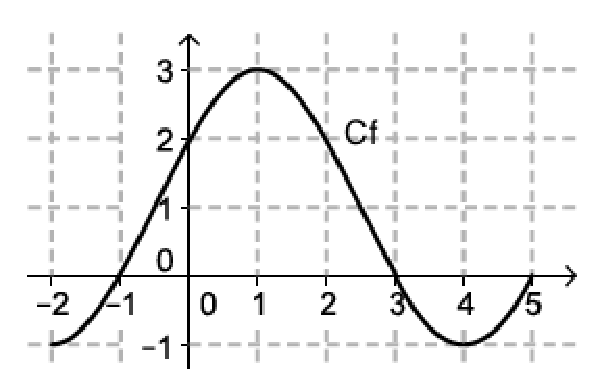
\includegraphics[scale=0.75]{Fonctions/figures/Ex1.eps}
\begin{enumerate}
\item Lire graphiquement l'image de 2, puis celle de 4 par $f$.
\item Lire graphiquement $f(3)$, puis $f(-2)$.
\item Combien 0 a-t'il de préimage par $f$?
\item Donner les préimages de 0.
\item Donner les préimages éventuelles de 2.
\item Combien - 2 a-t'il de préimages?
\end{enumerate}
\end{exercice}

\begin{exercice}
Voici la courbe représentative d'une fonction $h$. 
\begin{center}
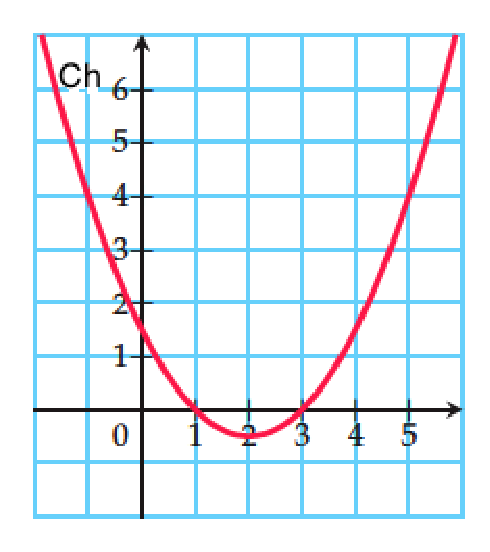
\includegraphics[scale=0.5]{Fonctions/figures/Ex3.eps}
\end{center}
\begin{enumerate}
\item Déterminer les images de:
\setlength{\columnseprule}{0pt}
\begin{multicols}{4}
\textbf{a)} 3

 \textbf{b)} 5
 
 \textbf{c)} 0
 
 \textbf{d)} -1
 \end{multicols}
 \vspace{0.5cm}
 \item Déterminer les pré images éventuelles de:
 \setlength{\columnseprule}{0pt}
\begin{multicols}{4}
\textbf{a)} 3

 \textbf{b)} 5
 
 \textbf{c)} 0
 
 \textbf{d)} -1
 \end{multicols}

\end{enumerate}
\end{exercice}

\begin{exercice}
Le tableau suivant est un tableau de valeurs correspondant à une fonction $f$ :
\begin{center}
\begin{tabular}{|l|c|c|c|c|c|c|} \hline
$x$ & -7 & -3,5 & 0 & 1 & 2 & 5 \\ \hline
$f(x$)  & 4 & -2 & -3& 3,5& 5 &-2   \\ \hline
\end{tabular} 
\end{center}
\begin{enumerate}
\item Donner la (ou les) préimage(s) des nombres suivants par la fonction $f$ : \newline
a. 3,5 $\qquad$ b.  -2  $\qquad$ c. 4;
\item Donner l'image de 2;
Que vaut $f(-3,5)$?
\end{enumerate}
\end{exercice}

\begin{exercice}
Soit $f$ une fonction définie sur $\mathbb{R}$ par $f(x)=3x-1$. 
\begin{enumerate}
\item Déterminer $f(1)$, $f(0)$, $f(-2)$.
\item Trouver la ou les préimage(s) de 0 par $f$
\item Trouver la ou les préimage(s) de 1 par $f$
\end{enumerate}
\end{exercice}

\begin{exercice}
Soit la fonction $f$ définie par $f(x)=-\dfrac{2}{3}x+1$.
\begin{enumerate}
\item Calculer l'image de 27 par $f$.
\item Calculer $f(-1)$
\item Déterminer la préimage de 1 par $f$.
\item -12 est-il une préimage de 8 par $f$?
\end{enumerate}
\end{exercice}

\begin{exercice}
Soit $g$ une fonction définie sur $\mathbb{R}$ par $g(x)=x^2-x-6$. 
\begin{enumerate}
\item Déterminer $g(2)$, $g(4)$, $g(-1)$, $g(\sqrt{3})$.
\item Trouver la ou les préimage(s) de $0$ par $g$
\end{enumerate}
\end{exercice}

\begin{exercice}
Traduire chaque égalité par une phrase contenant le mot "image" :

\begin{multicols}{2}
\begin{enumerate}
\item $f(3)=5$
\item $g(-1)=2$
\item $h(x)=x^2-5x$
\item $i(a)=-2a+1$
\end{enumerate}
 \end{multicols}
\end{exercice}

\begin{exercice}
On considère la fonction $f$ définie sur $\mathbb{R}$ par $f(x)=x^2-1$
\begin{enumerate}
\item Déterminer $f(0)$, $f(-1)$, $f(2)$.
\item En utilisant une identité remarquable, trouver les pré images de $0$ par $f$.
\end{enumerate}
\end{exercice}

\serie{Notions de fonctions}

\begin{exercice}
Choisir la bonne réponse :
\begin{enumerate}
\item La vitesse $V$ d'un véhicule est une fonction $h$ de la distance parcourue $D$. On note alors : \newline
\hspace*{1 cm} $\square\quad D=h(V)$  \hspace*{1.5 cm} $\square \quad V=h(D)$
\item Le nombre $N$ de noyaux radioactifs présents dans un échantillon de plutonium à la date $t$ est représenté par la fonction $f$. On note alors : \newline
\hspace*{1 cm} $\square\quad N=f(t)$ \hspace*{1 cm} $\square\quad t=f(N) $ 
\item L'allongement $L$ d'un ressort est fonction de la masse $m$ que l'on suspend. On note $g$ cette fonction. On note alors : \newline
\hspace*{1 cm} $\square\quad L=g(m)$ \hspace*{1 cm} $\square\quad m=g(L) $ 
\end{enumerate}
\end{exercice}

\begin{exercice}
Recopier et compléter les assertions suivantes :
\begin{enumerate}
\item On sait que 1 a pour préimage -2 par la fonction $f$, donc : 
\begin{itemize}
\item $f(\ldots)=\ldots$ 
\item \ldots a pour image \ldots par la fonction $f$
\item le point de coordonnées (\ldots;\ldots) appartient  à la courbe représentative de la fonction $f$.
\end{itemize}
\item On sait que 2 a pour image 0 par la fonction $f$, donc :
\begin{itemize}
\item $f(\ldots)=\ldots$ 
\item  \ldots a pour préimage \ldots par la fonction $f$
\item le point de coordonnées (\ldots;\ldots) appartient  à la courbe représentative de la fonction $f$.
\end{itemize}
\item On sait que le point de coordonnées (-4 ; 2) appartient à la courbe représentative de la fonction $f$. donc :  
\begin{itemize}
\item $f(\ldots)=\ldots$ 
\item \ldots a pour image \ldots par la fonction $f$ 
\item \ldots a pour préimage \ldots par la fonction $f$
\end{itemize}
\end{enumerate}
\end{exercice}

\begin{exercice}
Parmi les graphiques proposés, lesquels  correspondent à la représentation graphique d'une fonction?

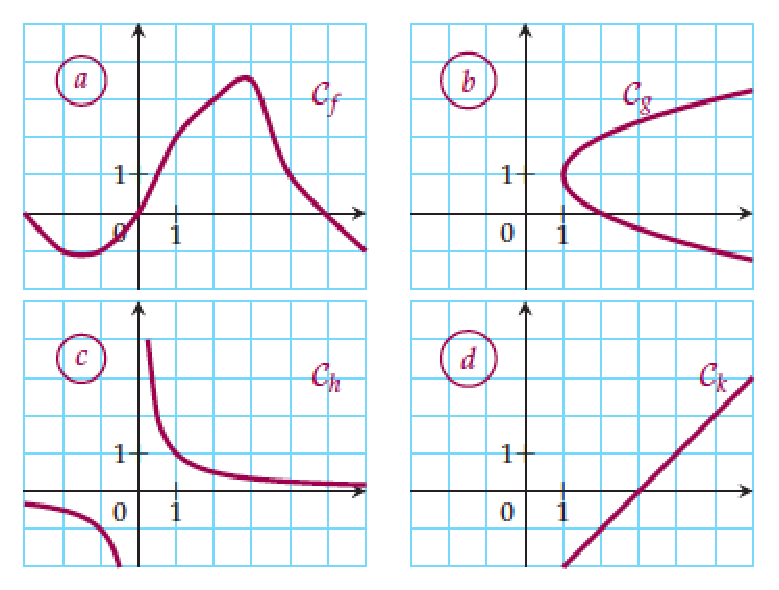
\includegraphics[scale=0.6]{Ex11}
\end{exercice}

\begin{exercice}
On considère un rectangle ABCD tel que AB = 10 et AD = 8.\\
On place E sur [AD] et on appelle F le point d'intersection de la parallèle à (BD) passant par E et du segment [AB].\\
On pose $x=$AE.

\begin{tikzpicture}[line cap=round,line join=round,>=triangle 45,x=1.0cm,y=1.0cm]
\clip(-1.8,0.7) rectangle (3.7,4.82);
\draw (-1.,4.)-- (3.,4.);
\draw (3.,4.)-- (3.,1.52);
\draw (-1.,4.)-- (-1.,1.52);
\draw (-1.,1.52)-- (3.,1.52);
\draw (-1.,1.52)-- (3.,4.);
\draw (-1.,2.)-- (2.22580645161,4.);
\begin{scriptsize}
\draw [color=black] (-1.,4.)-- ++(-0.5pt,-0.5pt) -- ++(1.0pt,1.0pt) ++(-1.0pt,0) -- ++(1.0pt,-1.0pt);
\draw[color=black] (-1.06,4.24) node {$A$};
\draw [color=black] (3.,4.)-- ++(-0.5pt,-0.5pt) -- ++(1.0pt,1.0pt) ++(-1.0pt,0) -- ++(1.0pt,-1.0pt);
\draw[color=black] (3.14,4.2) node {$B$};
\draw [color=black] (3.,1.52)-- ++(-0.5pt,-0.5pt) -- ++(1.0pt,1.0pt) ++(-1.0pt,0) -- ++(1.0pt,-1.0pt);
\draw[color=black] (3.12,1.44) node {$C$};
\draw [color=black] (-1.,1.52)-- ++(-0.5pt,-0.5pt) -- ++(1.0pt,1.0pt) ++(-1.0pt,0) -- ++(1.0pt,-1.0pt);
\draw[color=black] (-1.2,1.42) node {$D$};
\draw [color=black] (-1.,2.)-- ++(-0.5pt,-0.5pt) -- ++(1.0pt,1.0pt) ++(-1.0pt,0) -- ++(1.0pt,-1.0pt);
\draw[color=black] (-1.2,2.06) node {$E$};
\draw [color=black] (2.22580645161,4.)-- ++(-0.5pt,-0.5pt) -- ++(1.0pt,1.0pt) ++(-1.0pt,0) -- ++(1.0pt,-1.0pt);
\draw[color=black] (2.24,4.26) node {$F$};
\end{scriptsize}
\end{tikzpicture}
\begin{enumerate}
\item Quelles valeurs $x$ peut-elle prendre?
\item Exprimer, en fonction de $x$:
\begin{enumerate}
\item les longueurs ED et AF;
\item l'aire du triangle AEF.
\end{enumerate}
\end{enumerate}
\end{exercice}

\begin{exercice}
Sachant que la somme de deux nombres vaut 9, exprimer l'un des nombres en fonction de l'autre.
\end{exercice}

\begin{exercice}
On considère le programme de calcul suivant : 
\begin{itemize}
\item Choisir le nombre
\item Le multiplier par -2
\item Au résultat obtenu, retrancher 1
\end{itemize}
\begin{enumerate}
\item Déterminer l'expression de $f(x)$;
\item Compléter ci-dessous, le tableau suivant : 
\begin{center}
\renewcommand{\arraystretch}{2.33}
\begin{tabular}{|p{0.7cm}|p{0.7cm}|p{0.7cm}|p{0.7cm}|p{0.7cm}|p{0.7cm}|} 
 \hline
$x$&-2&-1&0&1&2\\\hline
$f(x)$&&&&&\\\hline
 \end{tabular}
\end{center}

\item Placer ces points dans un repère et tracer la courbe représentant la fontion $f$ sur l'intervalle [-2;2].\\
\end{enumerate}
\end{exercice}

\serie{Ensemble de définitions}

\begin{exercice}
\begin{enumerate}
\item Donner l'ensemble de définition, $\mathcal{D}_f$ de la fonction $f$ définie par $f(x)=\dfrac{3x-1}{x+1}$;

\item Donner sous forme d'intervalle l'ensemble de définition, $\mathcal{D}_g$ de la fonction $g$ définie par $g(x)=\sqrt{3x+4}$;

\item Déterminez $f(-2)$ et $g(5)$.
\end{enumerate}
\end{exercice}

\begin{exercice}
\begin{enumerate}
\item Donner l'ensemble de définition, $\mathcal{D}_f$ de la fonction $f$ définie par $f(x)=\dfrac{-5x-6}{{x^2-1}}$;

\item Donner sous forme d'intervalle l'ensemble de définition, $\mathcal{D}_g$ de la fonction $g$ définie par $g(x)=\sqrt{-2x+1}$;

\item Déterminez $f(1)$ et $g(1)$.
\end{enumerate}
\end{exercice}

\begin{exercice}
On considère la fonction $f$ dont la représentation graphique est donnée ci-dessous
\begin{center}
	\definecolor{qqqqff}{rgb}{0.,0.,1.}
\definecolor{cqcqcq}{rgb}{0.7529411764705882,0.7529411764705882,0.7529411764705882}
\begin{tikzpicture}[line cap=round,line join=round,>=triangle 45,x=1.0cm,y=1.0cm]
\draw [color=cqcqcq,, xstep=1.0cm,ystep=1.0cm] (-2.0846666666666667,-3.593333333333334) grid (3.87333333333334,2.606666666666668);
\draw[->,color=black] (-2.0846666666666667,0.) -- (3.87333333333334,0.);
\foreach \x in {-2.,-1.,1.,2.,3.}
\draw[shift={(\x,0)},color=black] (0pt,2pt) -- (0pt,-2pt) node[below] {\footnotesize $\x$};
\draw[->,color=black] (0.,-3.593333333333334) -- (0.,2.606666666666668);
\foreach \y in {-3.,-2.,-1.,1.,2.}
\draw[shift={(0,\y)},color=black] (2pt,0pt) -- (-2pt,0pt) node[left] {\footnotesize $\y$};
\draw[color=black] (0pt,-10pt) node[right] {\footnotesize $0$};
\clip(-2.0846666666666667,-3.593333333333334) rectangle (3.87333333333334,2.606666666666668);
\draw[line width=1.2pt,color=qqqqff] (-1.9999975286666603,29.999867783846497) -- (-1.9999975286666603,29.999867783846497);
\draw[line width=1.2pt,color=qqqqff] (-1.9999975286666603,29.999867783846497) -- (-1.987497538842973,29.33571682778489);
\draw[line width=1.2pt,color=qqqqff] (-1.987497538842973,29.33571682778489) -- (-1.9749975490192857,28.6807085909204);
\draw[line width=1.2pt,color=qqqqff] (-1.9749975490192857,28.6807085909204) -- (-1.9624975591955984,28.034767341073692);
\draw[line width=1.2pt,color=qqqqff] (-1.9624975591955984,28.034767341073692) -- (-1.9499975693719112,27.397817639033214);
\draw[line width=1.2pt,color=qqqqff] (-1.9499975693719112,27.397817639033214) -- (-1.9374975795482239,26.769784338555205);
\draw[line width=1.2pt,color=qqqqff] (-1.9374975795482239,26.769784338555205) -- (-1.9249975897245366,26.150592586363697);
\draw[line width=1.2pt,color=qqqqff] (-1.9249975897245366,26.150592586363697) -- (-1.9124975999008493,25.540167822150526);
\draw[line width=1.2pt,color=qqqqff] (-1.9124975999008493,25.540167822150526) -- (-1.899997610077162,24.938435778575336);
\draw[line width=1.2pt,color=qqqqff] (-1.899997610077162,24.938435778575336) -- (-1.8874976202534748,24.345322481265548);
\draw[line width=1.2pt,color=qqqqff] (-1.8874976202534748,24.345322481265548) -- (-1.8749976304297875,23.76075424881637);
\draw[line width=1.2pt,color=qqqqff] (-1.8749976304297875,23.76075424881637) -- (-1.8624976406061002,23.184657692790843);
\draw[line width=1.2pt,color=qqqqff] (-1.8624976406061002,23.184657692790843) -- (-1.849997650782413,22.616959717719777);
\draw[line width=1.2pt,color=qqqqff] (-1.849997650782413,22.616959717719777) -- (-1.8374976609587257,22.05758752110178);
\draw[line width=1.2pt,color=qqqqff] (-1.8374976609587257,22.05758752110178) -- (-1.8249976711350384,21.50646859340325);
\draw[line width=1.2pt,color=qqqqff] (-1.8249976711350384,21.50646859340325) -- (-1.8124976813113511,20.963530718058394);
\draw[line width=1.2pt,color=qqqqff] (-1.8124976813113511,20.963530718058394) -- (-1.7999976914876639,20.428701971469227);
\draw[line width=1.2pt,color=qqqqff] (-1.7999976914876639,20.428701971469227) -- (-1.7874977016639766,19.90191072300553);
\draw[line width=1.2pt,color=qqqqff] (-1.7874977016639766,19.90191072300553) -- (-1.7749977118402893,19.383085635004885);
\draw[line width=1.2pt,color=qqqqff] (-1.7749977118402893,19.383085635004885) -- (-1.762497722016602,18.872155662772695);
\draw[line width=1.2pt,color=qqqqff] (-1.762497722016602,18.872155662772695) -- (-1.7499977321929148,18.369050054582143);
\draw[line width=1.2pt,color=qqqqff] (-1.7499977321929148,18.369050054582143) -- (-1.7374977423692275,17.8736983516742);
\draw[line width=1.2pt,color=qqqqff] (-1.7374977423692275,17.8736983516742) -- (-1.7249977525455402,17.38603038825764);
\draw[line width=1.2pt,color=qqqqff] (-1.7249977525455402,17.38603038825764) -- (-1.712497762721853,16.90597629150903);
\draw[line width=1.2pt,color=qqqqff] (-1.712497762721853,16.90597629150903) -- (-1.6999977728981657,16.433466481572754);
\draw[line width=1.2pt,color=qqqqff] (-1.6999977728981657,16.433466481572754) -- (-1.6874977830744784,15.96843167156096);
\draw[line width=1.2pt,color=qqqqff] (-1.6874977830744784,15.96843167156096) -- (-1.6749977932507911,15.510802867553606);
\draw[line width=1.2pt,color=qqqqff] (-1.6749977932507911,15.510802867553606) -- (-1.6624978034271038,15.060511368598455);
\draw[line width=1.2pt,color=qqqqff] (-1.6624978034271038,15.060511368598455) -- (-1.6499978136034166,14.617488766711052);
\draw[line width=1.2pt,color=qqqqff] (-1.6499978136034166,14.617488766711052) -- (-1.6374978237797293,14.181666946874751);
\draw[line width=1.2pt,color=qqqqff] (-1.6374978237797293,14.181666946874751) -- (-1.624997833956042,13.75297808704068);
\draw[line width=1.2pt,color=qqqqff] (-1.624997833956042,13.75297808704068) -- (-1.6124978441323548,13.331354658127784);
\draw[line width=1.2pt,color=qqqqff] (-1.6124978441323548,13.331354658127784) -- (-1.5999978543086675,12.916729424022806);
\draw[line width=1.2pt,color=qqqqff] (-1.5999978543086675,12.916729424022806) -- (-1.5874978644849802,12.50903544158027);
\draw[line width=1.2pt,color=qqqqff] (-1.5874978644849802,12.50903544158027) -- (-1.574997874661293,12.108206060622498);
\draw[line width=1.2pt,color=qqqqff] (-1.574997874661293,12.108206060622498) -- (-1.5624978848376057,11.714174923939616);
\draw[line width=1.2pt,color=qqqqff] (-1.5624978848376057,11.714174923939616) -- (-1.5499978950139184,11.326875967289547);
\draw[line width=1.2pt,color=qqqqff] (-1.5499978950139184,11.326875967289547) -- (-1.537497905190231,10.946243419398002);
\draw[line width=1.2pt,color=qqqqff] (-1.537497905190231,10.946243419398002) -- (-1.5249979153665438,10.572211801958485);
\draw[line width=1.2pt,color=qqqqff] (-1.5249979153665438,10.572211801958485) -- (-1.5124979255428566,10.204715929632306);
\draw[line width=1.2pt,color=qqqqff] (-1.5124979255428566,10.204715929632306) -- (-1.4999979357191693,9.843690910048577);
\draw[line width=1.2pt,color=qqqqff] (-1.4999979357191693,9.843690910048577) -- (-1.487497945895482,9.489072143804185);
\draw[line width=1.2pt,color=qqqqff] (-1.487497945895482,9.489072143804185) -- (-1.4749979560717947,9.140795324463824);
\draw[line width=1.2pt,color=qqqqff] (-1.4749979560717947,9.140795324463824) -- (-1.4624979662481075,8.798796438559988);
\draw[line width=1.2pt,color=qqqqff] (-1.4624979662481075,8.798796438559988) -- (-1.4499979764244202,8.463011765592967);
\draw[line width=1.2pt,color=qqqqff] (-1.4499979764244202,8.463011765592967) -- (-1.437497986600733,8.133377878030835);
\draw[line width=1.2pt,color=qqqqff] (-1.437497986600733,8.133377878030835) -- (-1.4249979967770456,7.809831641309471);
\draw[line width=1.2pt,color=qqqqff] (-1.4249979967770456,7.809831641309471) -- (-1.4124980069533584,7.492310213832552);
\draw[line width=1.2pt,color=qqqqff] (-1.4124980069533584,7.492310213832552) -- (-1.399998017129671,7.180751046971553);
\draw[line width=1.2pt,color=qqqqff] (-1.399998017129671,7.180751046971553) -- (-1.3874980273059838,6.875091885065731);
\draw[line width=1.2pt,color=qqqqff] (-1.3874980273059838,6.875091885065731) -- (-1.3749980374822965,6.575270765422149);
\draw[line width=1.2pt,color=qqqqff] (-1.3749980374822965,6.575270765422149) -- (-1.3624980476586093,6.28122601831567);
\draw[line width=1.2pt,color=qqqqff] (-1.3624980476586093,6.28122601831567) -- (-1.349998057834922,5.992896266988946);
\draw[line width=1.2pt,color=qqqqff] (-1.349998057834922,5.992896266988946) -- (-1.3374980680112347,5.710220427652425);
\draw[line width=1.2pt,color=qqqqff] (-1.3374980680112347,5.710220427652425) -- (-1.3249980781875474,5.433137709484354);
\draw[line width=1.2pt,color=qqqqff] (-1.3249980781875474,5.433137709484354) -- (-1.3124980883638602,5.161587614630773);
\draw[line width=1.2pt,color=qqqqff] (-1.3124980883638602,5.161587614630773) -- (-1.299998098540173,4.8955099382055245);
\draw[line width=1.2pt,color=qqqqff] (-1.299998098540173,4.8955099382055245) -- (-1.2874981087164856,4.634844768290238);
\draw[line width=1.2pt,color=qqqqff] (-1.2874981087164856,4.634844768290238) -- (-1.2749981188927983,4.379532485934342);
\draw[line width=1.2pt,color=qqqqff] (-1.2749981188927983,4.379532485934342) -- (-1.262498129069111,4.129513765155067);
\draw[line width=1.2pt,color=qqqqff] (-1.262498129069111,4.129513765155067) -- (-1.2499981392454238,3.8847295729374323);
\draw[line width=1.2pt,color=qqqqff] (-1.2499981392454238,3.8847295729374323) -- (-1.2374981494217365,3.645121169234256);
\draw[line width=1.2pt,color=qqqqff] (-1.2374981494217365,3.645121169234256) -- (-1.2249981595980493,3.410630106966149);
\draw[line width=1.2pt,color=qqqqff] (-1.2249981595980493,3.410630106966149) -- (-1.212498169774362,3.181198232021523);
\draw[line width=1.2pt,color=qqqqff] (-1.212498169774362,3.181198232021523) -- (-1.1999981799506747,2.956767683256585);
\draw[line width=1.2pt,color=qqqqff] (-1.1999981799506747,2.956767683256585) -- (-1.1874981901269874,2.737280892495335);
\draw[line width=1.2pt,color=qqqqff] (-1.1874981901269874,2.737280892495335) -- (-1.1749982003033002,2.522680584529569);
\draw[line width=1.2pt,color=qqqqff] (-1.1749982003033002,2.522680584529569) -- (-1.1624982104796129,2.312909777118883);
\draw[line width=1.2pt,color=qqqqff] (-1.1624982104796129,2.312909777118883) -- (-1.1499982206559256,2.107911780990666);
\draw[line width=1.2pt,color=qqqqff] (-1.1499982206559256,2.107911780990666) -- (-1.1374982308322383,1.9076301998401026);
\draw[line width=1.2pt,color=qqqqff] (-1.1374982308322383,1.9076301998401026) -- (-1.124998241008551,1.7120089303301735);
\draw[line width=1.2pt,color=qqqqff] (-1.124998241008551,1.7120089303301735) -- (-1.1124982511848638,1.5209921620916569);
\draw[line width=1.2pt,color=qqqqff] (-1.1124982511848638,1.5209921620916569) -- (-1.0999982613611765,1.334524377723127);
\draw[line width=1.2pt,color=qqqqff] (-1.0999982613611765,1.334524377723127) -- (-1.0874982715374892,1.1525503527909522);
\draw[line width=1.2pt,color=qqqqff] (-1.0874982715374892,1.1525503527909522) -- (-1.074998281713802,0.9750151558292969);
\draw[line width=1.2pt,color=qqqqff] (-1.074998281713802,0.9750151558292969) -- (-1.0624982918901147,0.8018641483401238);
\draw[line width=1.2pt,color=qqqqff] (-1.0624982918901147,0.8018641483401238) -- (-1.0499983020664274,0.6330429847931895);
\draw[line width=1.2pt,color=qqqqff] (-1.0499983020664274,0.6330429847931895) -- (-1.0374983122427401,0.4684976126260472);
\draw[line width=1.2pt,color=qqqqff] (-1.0374983122427401,0.4684976126260472) -- (-1.0249983224190529,0.3081742722440458);
\draw[line width=1.2pt,color=qqqqff] (-1.0249983224190529,0.3081742722440458) -- (-1.0124983325953656,0.1520194970203307);
\draw[line width=1.2pt,color=qqqqff] (-1.0124983325953656,0.1520194970203307) -- (-0.9999983427716783,0.0);
\draw[line width=1.2pt,color=qqqqff] (-0.9999983427716783,0.0) -- (-0.987498352947991,-0.14799675962068026);
\draw[line width=1.2pt,color=qqqqff] (-0.987498352947991,-0.14799675962068026) -- (-0.9749983631243038,-0.2919637094527061);
\draw[line width=1.2pt,color=qqqqff] (-0.9749983631243038,-0.2919637094527061) -- (-0.9624983733006165,-0.43197303095590556);
\draw[line width=1.2pt,color=qqqqff] (-0.9624983733006165,-0.43197303095590556) -- (-0.9499983834769292,-0.5680767259181536);
\draw[line width=1.2pt,color=qqqqff] (-0.9499983834769292,-0.5680767259181536) -- (-0.937498393653242,-0.7003265031595294);
\draw[line width=1.2pt,color=qqqqff] (-0.937498393653242,-0.7003265031595294) -- (-0.9249984038295547,-0.8287737785323157);
\draw[line width=1.2pt,color=qqqqff] (-0.9249984038295547,-0.8287737785323157) -- (-0.9124984140058674,-0.9534696749209998);
\draw[line width=1.2pt,color=qqqqff] (-0.9124984140058674,-0.9534696749209998) -- (-0.8999984241821801,-1.074465022242273);
\draw[line width=1.2pt,color=qqqqff] (-0.8999984241821801,-1.074465022242273) -- (-0.8874984343584928,-1.1918103574450307);
\draw[line width=1.2pt,color=qqqqff] (-0.8874984343584928,-1.1918103574450307) -- (-0.8749984445348056,-1.305555924510371);
\draw[line width=1.2pt,color=qqqqff] (-0.8749984445348056,-1.305555924510371) -- (-0.8624984547111183,-1.415751674451598);
\draw[line width=1.2pt,color=qqqqff] (-0.8624984547111183,-1.415751674451598) -- (-0.849998464887431,-1.5224472653142191);
\draw[line width=1.2pt,color=qqqqff] (-0.849998464887431,-1.5224472653142191) -- (-0.8374984750637438,-1.6256920621759456);
\draw[line width=1.2pt,color=qqqqff] (-0.8374984750637438,-1.6256920621759456) -- (-0.8249984852400565,-1.7255351371466916);
\draw[line width=1.2pt,color=qqqqff] (-0.8249984852400565,-1.7255351371466916) -- (-0.8124984954163692,-1.8220252693685777);
\draw[line width=1.2pt,color=qqqqff] (-0.8124984954163692,-1.8220252693685777) -- (-0.7999985055926819,-1.9152109450159271);
\draw[line width=1.2pt,color=qqqqff] (-0.7999985055926819,-1.9152109450159271) -- (-0.7874985157689947,-2.005140357295267);
\draw[line width=1.2pt,color=qqqqff] (-0.7874985157689947,-2.005140357295267) -- (-0.7749985259453074,-2.091861406445328);
\draw[line width=1.2pt,color=qqqqff] (-0.7749985259453074,-2.091861406445328) -- (-0.7624985361216201,-2.1754216997370466);
\draw[line width=1.2pt,color=qqqqff] (-0.7624985361216201,-2.1754216997370466) -- (-0.7499985462979328,-2.255868551473563);
\draw[line width=1.2pt,color=qqqqff] (-0.7499985462979328,-2.255868551473563) -- (-0.7374985564742456,-2.333248982990219);
\draw[line width=1.2pt,color=qqqqff] (-0.7374985564742456,-2.333248982990219) -- (-0.7249985666505583,-2.4076097226545623);
\draw[line width=1.2pt,color=qqqqff] (-0.7249985666505583,-2.4076097226545623) -- (-0.712498576826871,-2.478997205866345);
\draw[line width=1.2pt,color=qqqqff] (-0.712498576826871,-2.478997205866345) -- (-0.6999985870031837,-2.547457575057524);
\draw[line width=1.2pt,color=qqqqff] (-0.6999985870031837,-2.547457575057524) -- (-0.6874985971794965,-2.6130366796922564);
\draw[line width=1.2pt,color=qqqqff] (-0.6874985971794965,-2.6130366796922564) -- (-0.6749986073558092,-2.6757800762669075);
\draw[line width=1.2pt,color=qqqqff] (-0.6749986073558092,-2.6757800762669075) -- (-0.6624986175321219,-2.7357330283100434);
\draw[line width=1.2pt,color=qqqqff] (-0.6624986175321219,-2.7357330283100434) -- (-0.6499986277084346,-2.792940506382439);
\draw[line width=1.2pt,color=qqqqff] (-0.6499986277084346,-2.792940506382439) -- (-0.6374986378847474,-2.847447188077067);
\draw[line width=1.2pt,color=qqqqff] (-0.6374986378847474,-2.847447188077067) -- (-0.6249986480610601,-2.899297458019107);
\draw[line width=1.2pt,color=qqqqff] (-0.6249986480610601,-2.899297458019107) -- (-0.6124986582373728,-2.9485354078659447);
\draw[line width=1.2pt,color=qqqqff] (-0.6124986582373728,-2.9485354078659447) -- (-0.5999986684136855,-2.9952048363071673);
\draw[line width=1.2pt,color=qqqqff] (-0.5999986684136855,-2.9952048363071673) -- (-0.5874986785899983,-3.039349249064567);
\draw[line width=1.2pt,color=qqqqff] (-0.5874986785899983,-3.039349249064567) -- (-0.574998688766311,-3.081011858892137);
\draw[line width=1.2pt,color=qqqqff] (-0.574998688766311,-3.081011858892137) -- (-0.5624986989426237,-3.120235585576081);
\draw[line width=1.2pt,color=qqqqff] (-0.5624986989426237,-3.120235585576081) -- (-0.5499987091189364,-3.157063055934801);
\draw[line width=1.2pt,color=qqqqff] (-0.5499987091189364,-3.157063055934801) -- (-0.5374987192952492,-3.1915366038189057);
\draw[line width=1.2pt,color=qqqqff] (-0.5374987192952492,-3.1915366038189057) -- (-0.5249987294715619,-3.2236982701112047);
\draw[line width=1.2pt,color=qqqqff] (-0.5249987294715619,-3.2236982701112047) -- (-0.5124987396478746,-3.2535898027267165);
\draw[line width=1.2pt,color=qqqqff] (-0.5124987396478746,-3.2535898027267165) -- (-0.49999874982418735,-3.2812526566126614);
\draw[line width=1.2pt,color=qqqqff] (-0.49999874982418735,-3.2812526566126614) -- (-0.4874987600005001,-3.306727993748462);
\draw[line width=1.2pt,color=qqqqff] (-0.4874987600005001,-3.306727993748462) -- (-0.4749987701768128,-3.330056683145747);
\draw[line width=1.2pt,color=qqqqff] (-0.4749987701768128,-3.330056683145747) -- (-0.4624987803531255,-3.351279300848348);
\draw[line width=1.2pt,color=qqqqff] (-0.4624987803531255,-3.351279300848348) -- (-0.44999879052943825,-3.3704361299323025);
\draw[line width=1.2pt,color=qqqqff] (-0.44999879052943825,-3.3704361299323025) -- (-0.437498800705751,-3.3875671605058497);
\draw[line width=1.2pt,color=qqqqff] (-0.437498800705751,-3.3875671605058497) -- (-0.4249988108820637,-3.402712089709433);
\draw[line width=1.2pt,color=qqqqff] (-0.4249988108820637,-3.402712089709433) -- (-0.41249882105837643,-3.4159103217157014);
\draw[line width=1.2pt,color=qqqqff] (-0.41249882105837643,-3.4159103217157014) -- (-0.39999883123468916,-3.427200967729509);
\draw[line width=1.2pt,color=qqqqff] (-0.39999883123468916,-3.427200967729509) -- (-0.3874988414110019,-3.4366228459879093);
\draw[line width=1.2pt,color=qqqqff] (-0.3874988414110019,-3.4366228459879093) -- (-0.3749988515873146,-3.4442144817601634);
\draw[line width=1.2pt,color=qqqqff] (-0.3749988515873146,-3.4442144817601634) -- (-0.36249886176362733,-3.4500141073477355);
\draw[line width=1.2pt,color=qqqqff] (-0.36249886176362733,-3.4500141073477355) -- (-0.34999887193994006,-3.4540596620842954);
\draw[line width=1.2pt,color=qqqqff] (-0.34999887193994006,-3.4540596620842954) -- (-0.3374988821162528,-3.4563887923357157);
\draw[line width=1.2pt,color=qqqqff] (-0.3374988821162528,-3.4563887923357157) -- (-0.3249988922925655,-3.4570388515000694);
\draw[line width=1.2pt,color=qqqqff] (-0.3249988922925655,-3.4570388515000694) -- (-0.31249890246887824,-3.4560469000076397);
\draw[line width=1.2pt,color=qqqqff] (-0.31249890246887824,-3.4560469000076397) -- (-0.29999891264519096,-3.4534497053209114);
\draw[line width=1.2pt,color=qqqqff] (-0.29999891264519096,-3.4534497053209114) -- (-0.2874989228215037,-3.449283741934572);
\draw[line width=1.2pt,color=qqqqff] (-0.2874989228215037,-3.449283741934572) -- (-0.2749989329978164,-3.4435851913755138);
\draw[line width=1.2pt,color=qqqqff] (-0.2749989329978164,-3.4435851913755138) -- (-0.26249894317412914,-3.436389942202834);
\draw[line width=1.2pt,color=qqqqff] (-0.26249894317412914,-3.436389942202834) -- (-0.24999895335044187,-3.4277335900078336);
\draw[line width=1.2pt,color=qqqqff] (-0.24999895335044187,-3.4277335900078336) -- (-0.2374989635267546,-3.4176514374140163);
\draw[line width=1.2pt,color=qqqqff] (-0.2374989635267546,-3.4176514374140163) -- (-0.22499897370306732,-3.4061784940770905);
\draw[line width=1.2pt,color=qqqqff] (-0.22499897370306732,-3.4061784940770905) -- (-0.21249898387938004,-3.39334947668497);
\draw[line width=1.2pt,color=qqqqff] (-0.21249898387938004,-3.39334947668497) -- (-0.19999899405569277,-3.3791988089577707);
\draw[line width=1.2pt,color=qqqqff] (-0.19999899405569277,-3.3791988089577707) -- (-0.1874990042320055,-3.363760621647815);
\draw[line width=1.2pt,color=qqqqff] (-0.1874990042320055,-3.363760621647815) -- (-0.17499901440831822,-3.3470687525396245);
\draw[line width=1.2pt,color=qqqqff] (-0.17499901440831822,-3.3470687525396245) -- (-0.16249902458463095,-3.32915674644993);
\draw[line width=1.2pt,color=qqqqff] (-0.16249902458463095,-3.32915674644993) -- (-0.14999903476094367,-3.310057855227665);
\draw[line width=1.2pt,color=qqqqff] (-0.14999903476094367,-3.310057855227665) -- (-0.1374990449372564,-3.289805037753966);
\draw[line width=1.2pt,color=qqqqff] (-0.1374990449372564,-3.289805037753966) -- (-0.12499905511356914,-3.2684309599421724);
\draw[line width=1.2pt,color=qqqqff] (-0.12499905511356914,-3.2684309599421724) -- (-0.11249906528988188,-3.245967994737831);
\draw[line width=1.2pt,color=qqqqff] (-0.11249906528988188,-3.245967994737831) -- (-0.09999907546619462,-3.2224482221186888);
\draw[line width=1.2pt,color=qqqqff] (-0.09999907546619462,-3.2224482221186888) -- (-0.08749908564250736,-3.1979034290947004);
\draw[line width=1.2pt,color=qqqqff] (-0.08749908564250736,-3.1979034290947004) -- (-0.0749990958188201,-3.1723651097080214);
\draw[line width=1.2pt,color=qqqqff] (-0.0749990958188201,-3.1723651097080214) -- (-0.06249910599513283,-3.1458644650330143);
\draw[line width=1.2pt,color=qqqqff] (-0.06249910599513283,-3.1458644650330143) -- (-0.04999911617144556,-3.118432403176243);
\draw[line width=1.2pt,color=qqqqff] (-0.04999911617144556,-3.118432403176243) -- (-0.037499126347758295,-3.090099539276478);
\draw[line width=1.2pt,color=qqqqff] (-0.037499126347758295,-3.090099539276478) -- (-0.024999136524071028,-3.06089619550469);
\draw[line width=1.2pt,color=qqqqff] (-0.024999136524071028,-3.06089619550469) -- (-0.012499146700383762,-3.0308524010640587);
\draw[line width=1.2pt,color=qqqqff] (-0.012499146700383762,-3.0308524010640587) -- (0.0,-2.9999978921899637);
\draw[line width=1.2pt,color=qqqqff] (0.0,-2.9999978921899637) -- (0.012499989823687266,-2.9683642716703846);
\draw[line width=1.2pt,color=qqqqff] (0.012499989823687266,-2.9683642716703846) -- (0.02499997964737453,-2.935976420518374);
\draw[line width=1.2pt,color=qqqqff] (0.02499997964737453,-2.935976420518374) -- (0.037499969471061795,-2.9028653038957235);
\draw[line width=1.2pt,color=qqqqff] (0.037499969471061795,-2.9028653038957235) -- (0.04999995929474906,-2.8690594861863894);
\draw[line width=1.2pt,color=qqqqff] (0.04999995929474906,-2.8690594861863894) -- (0.06249994911843633,-2.834587238806535);
\draw[line width=1.2pt,color=qqqqff] (0.06249994911843633,-2.834587238806535) -- (0.07499993894212359,-2.7994765402045254);
\draw[line width=1.2pt,color=qqqqff] (0.07499993894212359,-2.7994765402045254) -- (0.08749992876581085,-2.7637550758609324);
\draw[line width=1.2pt,color=qqqqff] (0.08749992876581085,-2.7637550758609324) -- (0.09999991858949811,-2.7274502382885277);
\draw[line width=1.2pt,color=qqqqff] (0.09999991858949811,-2.7274502382885277) -- (0.11249990841318537,-2.69058912703229);
\draw[line width=1.2pt,color=qqqqff] (0.11249990841318537,-2.69058912703229) -- (0.12499989823687263,-2.653198548669402);
\draw[line width=1.2pt,color=qqqqff] (0.12499989823687263,-2.653198548669402) -- (0.1374998880605599,-2.6153050168092498);
\draw[line width=1.2pt,color=qqqqff] (0.1374998880605599,-2.6153050168092498) -- (0.14999987788424718,-2.5769347520934236);
\draw[line width=1.2pt,color=qqqqff] (0.14999987788424718,-2.5769347520934236) -- (0.16249986770793445,-2.538113682195717);
\draw[line width=1.2pt,color=qqqqff] (0.16249986770793445,-2.538113682195717) -- (0.17499985753162173,-2.498867441822128);
\draw[line width=1.2pt,color=qqqqff] (0.17499985753162173,-2.498867441822128) -- (0.187499847355309,-2.4592213727108594);
\draw[line width=1.2pt,color=qqqqff] (0.187499847355309,-2.4592213727108594) -- (0.19999983717899628,-2.4192005236323184);
\draw[line width=1.2pt,color=qqqqff] (0.19999983717899628,-2.4192005236323184) -- (0.21249982700268355,-2.3788296503891138);
\draw[line width=1.2pt,color=qqqqff] (0.21249982700268355,-2.3788296503891138) -- (0.22499981682637082,-2.33813321581606);
\draw[line width=1.2pt,color=qqqqff] (0.22499981682637082,-2.33813321581606) -- (0.2374998066500581,-2.2971353897801765);
\draw[line width=1.2pt,color=qqqqff] (0.2374998066500581,-2.2971353897801765) -- (0.24999979647374537,-2.2558600491806846);
\draw[line width=1.2pt,color=qqqqff] (0.24999979647374537,-2.2558600491806846) -- (0.26249978629743265,-2.2143307779490113);
\draw[line width=1.2pt,color=qqqqff] (0.26249978629743265,-2.2143307779490113) -- (0.2749997761211199,-2.172570867048787);
\draw[line width=1.2pt,color=qqqqff] (0.2749997761211199,-2.172570867048787) -- (0.2874997659448072,-2.1306033144758456);
\draw[line width=1.2pt,color=qqqqff] (0.2874997659448072,-2.1306033144758456) -- (0.29999975576849447,-2.088450825258226);
\draw[line width=1.2pt,color=qqqqff] (0.29999975576849447,-2.088450825258226) -- (0.31249974559218174,-2.046135811456171);
\draw[line width=1.2pt,color=qqqqff] (0.31249974559218174,-2.046135811456171) -- (0.324999735415869,-2.003680392162127);
\draw[line width=1.2pt,color=qqqqff] (0.324999735415869,-2.003680392162127) -- (0.3374997252395563,-1.9611063935007438);
\draw[line width=1.2pt,color=qqqqff] (0.3374997252395563,-1.9611063935007438) -- (0.34999971506324357,-1.918435348628877);
\draw[line width=1.2pt,color=qqqqff] (0.34999971506324357,-1.918435348628877) -- (0.36249970488693084,-1.8756884977355848);
\draw[line width=1.2pt,color=qqqqff] (0.36249970488693084,-1.8756884977355848) -- (0.3749996947106181,-1.83288678804213);
\draw[line width=1.2pt,color=qqqqff] (0.3749996947106181,-1.83288678804213) -- (0.3874996845343054,-1.7900508738019794);
\draw[line width=1.2pt,color=qqqqff] (0.3874996845343054,-1.7900508738019794) -- (0.39999967435799266,-1.747201116300803);
\draw[line width=1.2pt,color=qqqqff] (0.39999967435799266,-1.747201116300803) -- (0.41249966418167994,-1.704357583856477);
\draw[line width=1.2pt,color=qqqqff] (0.41249966418167994,-1.704357583856477) -- (0.4249996540053672,-1.6615400518190782);
\draw[line width=1.2pt,color=qqqqff] (0.4249996540053672,-1.6615400518190782) -- (0.4374996438290545,-1.6187680025708913);
\draw[line width=1.2pt,color=qqqqff] (0.4374996438290545,-1.6187680025708913) -- (0.44999963365274176,-1.5760606255264018);
\draw[line width=1.2pt,color=qqqqff] (0.44999963365274176,-1.5760606255264018) -- (0.46249962347642903,-1.5334368171323014);
\draw[line width=1.2pt,color=qqqqff] (0.46249962347642903,-1.5334368171323014) -- (0.4749996133001163,-1.4909151808674843);
\draw[line width=1.2pt,color=qqqqff] (0.4749996133001163,-1.4909151808674843) -- (0.4874996031238036,-1.4485140272430501);
\draw[line width=1.2pt,color=qqqqff] (0.4874996031238036,-1.4485140272430501) -- (0.49999959294749086,-1.406251373802301);
\draw[line width=1.2pt,color=qqqqff] (0.49999959294749086,-1.406251373802301) -- (0.5124995827711781,-1.364144945120745);
\draw[line width=1.2pt,color=qqqqff] (0.5124995827711781,-1.364144945120745) -- (0.5249995725948654,-1.3222121728060918);
\draw[line width=1.2pt,color=qqqqff] (0.5249995725948654,-1.3222121728060918) -- (0.5374995624185527,-1.2804701954982576);
\draw[line width=1.2pt,color=qqqqff] (0.5374995624185527,-1.2804701954982576) -- (0.54999955224224,-1.2389358588693604);
\draw[line width=1.2pt,color=qqqqff] (0.54999955224224,-1.2389358588693604) -- (0.5624995420659272,-1.1976257156237244);
\draw[line width=1.2pt,color=qqqqff] (0.5624995420659272,-1.1976257156237244) -- (0.5749995318896145,-1.156556025497876);
\draw[line width=1.2pt,color=qqqqff] (0.5749995318896145,-1.156556025497876) -- (0.5874995217133018,-1.1157427552605466);
\draw[line width=1.2pt,color=qqqqff] (0.5874995217133018,-1.1157427552605466) -- (0.599999511536989,-1.075201578712671);
\draw[line width=1.2pt,color=qqqqff] (0.599999511536989,-1.075201578712671) -- (0.6124995013606763,-1.0349478766873887);
\draw[line width=1.2pt,color=qqqqff] (0.6124995013606763,-1.0349478766873887) -- (0.6249994911843636,-0.9949967370500429);
\draw[line width=1.2pt,color=qqqqff] (0.6249994911843636,-0.9949967370500429) -- (0.6374994810080509,-0.9553629546981808);
\draw[line width=1.2pt,color=qqqqff] (0.6374994810080509,-0.9553629546981808) -- (0.6499994708317381,-0.9160610315615538);
\draw[line width=1.2pt,color=qqqqff] (0.6499994708317381,-0.9160610315615538) -- (0.6624994606554254,-0.8771051766021173);
\draw[line width=1.2pt,color=qqqqff] (0.6624994606554254,-0.8771051766021173) -- (0.6749994504791127,-0.83850930581403);
\draw[line width=1.2pt,color=qqqqff] (0.6749994504791127,-0.83850930581403) -- (0.6874994403028,-0.8002870422236562);
\draw[line width=1.2pt,color=qqqqff] (0.6874994403028,-0.8002870422236562) -- (0.6999994301264872,-0.7624517158895624);
\draw[line width=1.2pt,color=qqqqff] (0.6999994301264872,-0.7624517158895624) -- (0.7124994199501745,-0.7250163639025209);
\draw[line width=1.2pt,color=qqqqff] (0.7124994199501745,-0.7250163639025209) -- (0.7249994097738618,-0.6879937303855063);
\draw[line width=1.2pt,color=qqqqff] (0.7249994097738618,-0.6879937303855063) -- (0.7374993995975491,-0.6513962664936989);
\draw[line width=1.2pt,color=qqqqff] (0.7374993995975491,-0.6513962664936989) -- (0.7499993894212363,-0.6152361304144814);
\draw[line width=1.2pt,color=qqqqff] (0.7499993894212363,-0.6152361304144814) -- (0.7624993792449236,-0.5795251873674419);
\draw[line width=1.2pt,color=qqqqff] (0.7624993792449236,-0.5795251873674419) -- (0.7749993690686109,-0.5442750096043717);
\draw[line width=1.2pt,color=qqqqff] (0.7749993690686109,-0.5442750096043717) -- (0.7874993588922982,-0.5094968764092664);
\draw[line width=1.2pt,color=qqqqff] (0.7874993588922982,-0.5094968764092664) -- (0.7999993487159854,-0.47520177409832576);
\draw[line width=1.2pt,color=qqqqff] (0.7999993487159854,-0.47520177409832576) -- (0.8124993385396727,-0.4414003960199535);
\draw[line width=1.2pt,color=qqqqff] (0.8124993385396727,-0.4414003960199535) -- (0.82499932836336,-0.40810314255475694);
\draw[line width=1.2pt,color=qqqqff] (0.82499932836336,-0.40810314255475694) -- (0.8374993181870473,-0.37532012111554813);
\draw[line width=1.2pt,color=qqqqff] (0.8374993181870473,-0.37532012111554813) -- (0.8499993080107345,-0.3430611461473426);
\draw[line width=1.2pt,color=qqqqff] (0.8499993080107345,-0.3430611461473426) -- (0.8624992978344218,-0.3113357391273602);
\draw[line width=1.2pt,color=qqqqff] (0.8624992978344218,-0.3113357391273602) -- (0.8749992876581091,-0.2801531285650246);
\draw[line width=1.2pt,color=qqqqff] (0.8749992876581091,-0.2801531285650246) -- (0.8874992774817964,-0.24952225000196385);
\draw[line width=1.2pt,color=qqqqff] (0.8874992774817964,-0.24952225000196385) -- (0.8999992673054836,-0.21945174601200954);
\draw[line width=1.2pt,color=qqqqff] (0.8999992673054836,-0.21945174601200954) -- (0.9124992571291709,-0.18994996620119772);
\draw[line width=1.2pt,color=qqqqff] (0.9124992571291709,-0.18994996620119772) -- (0.9249992469528582,-0.16102496720776818);
\draw[line width=1.2pt,color=qqqqff] (0.9249992469528582,-0.16102496720776818) -- (0.9374992367765455,-0.13268451270216494);
\draw[line width=1.2pt,color=qqqqff] (0.9374992367765455,-0.13268451270216494) -- (0.9499992266002327,-0.10493607338703587);
\draw[line width=1.2pt,color=qqqqff] (0.9499992266002327,-0.10493607338703587) -- (0.96249921642392,-0.07778682699723304);
\draw[line width=1.2pt,color=qqqqff] (0.96249921642392,-0.07778682699723304) -- (0.9749992062476073,-0.05124365829981237);
\draw[line width=1.2pt,color=qqqqff] (0.9749992062476073,-0.05124365829981237) -- (0.9874991960712945,-0.02531315909403397);
\draw[line width=1.2pt,color=qqqqff] (0.9874991960712945,-0.02531315909403397) -- (0.9999991858949818,0.0);
\draw[line width=1.2pt,color=qqqqff] (0.9999991858949818,0.0) -- (1.012499175718669,0.024684928484535563);
\draw[line width=1.2pt,color=qqqqff] (1.012499175718669,0.024684928484535563) -- (1.0249991655423563,0.04874079809778669);
\draw[line width=1.2pt,color=qqqqff] (1.0249991655423563,0.04874079809778669) -- (1.0374991553660435,0.07216056070031512);
\draw[line width=1.2pt,color=qqqqff] (1.0374991553660435,0.07216056070031512) -- (1.0499991451897308,0.09493908933184067);
\draw[line width=1.2pt,color=qqqqff] (1.0499991451897308,0.09493908933184067) -- (1.062499135013418,0.11707154999987915);
\draw[line width=1.2pt,color=qqqqff] (1.062499135013418,0.11707154999987915) -- (1.0749991248371054,0.13855340167974226);
\draw[line width=1.2pt,color=qqqqff] (1.0749991248371054,0.13855340167974226) -- (1.0874991146607926,0.15938039631453782);
\draw[line width=1.2pt,color=qqqqff] (1.0874991146607926,0.15938039631453782) -- (1.09999910448448,0.17954857881516953);
\draw[line width=1.2pt,color=qqqqff] (1.09999910448448,0.17954857881516953) -- (1.1124990943081672,0.19905428706033693);
\draw[line width=1.2pt,color=qqqqff] (1.1124990943081672,0.19905428706033693) -- (1.1249990841318545,0.21789415189653577);
\draw[line width=1.2pt,color=qqqqff] (1.1249990841318545,0.21789415189653577) -- (1.1374990739555417,0.23606509713805773);
\draw[line width=1.2pt,color=qqqqff] (1.1374990739555417,0.23606509713805773) -- (1.149999063779229,0.25356433956699037);
\draw[line width=1.2pt,color=qqqqff] (1.149999063779229,0.25356433956699037) -- (1.1624990536029163,0.2703893889332171);
\draw[line width=1.2pt,color=qqqqff] (1.1624990536029163,0.2703893889332171) -- (1.1749990434266036,0.28653804795441773);
\draw[line width=1.2pt,color=qqqqff] (1.1749990434266036,0.28653804795441773) -- (1.1874990332502908,0.30200841231606756);
\draw[line width=1.2pt,color=qqqqff] (1.1874990332502908,0.30200841231606756) -- (1.199999023073978,0.3167988706714382);
\draw[line width=1.2pt,color=qqqqff] (1.199999023073978,0.3167988706714382) -- (1.2124990128976654,0.33090810464159687);
\draw[line width=1.2pt,color=qqqqff] (1.2124990128976654,0.33090810464159687) -- (1.2249990027213526,0.3443350888154072);
\draw[line width=1.2pt,color=qqqqff] (1.2249990027213526,0.3443350888154072) -- (1.23749899254504,0.3570790907495286);
\draw[line width=1.2pt,color=qqqqff] (1.23749899254504,0.3570790907495286) -- (1.2499989823687272,0.3691396709684165);
\draw[line width=1.2pt,color=qqqqff] (1.2499989823687272,0.3691396709684165) -- (1.2624989721924145,0.3805166829643219);
\draw[line width=1.2pt,color=qqqqff] (1.2624989721924145,0.3805166829643219) -- (1.2749989620161017,0.3912102731972924);
\draw[line width=1.2pt,color=qqqqff] (1.2749989620161017,0.3912102731972924) -- (1.287498951839789,0.40122088109517123);
\draw[line width=1.2pt,color=qqqqff] (1.287498951839789,0.40122088109517123) -- (1.2999989416634763,0.4105492390535977);
\draw[line width=1.2pt,color=qqqqff] (1.2999989416634763,0.4105492390535977) -- (1.3124989314871636,0.4191963724360069);
\draw[line width=1.2pt,color=qqqqff] (1.3124989314871636,0.4191963724360069) -- (1.3249989213108508,0.42716359957363004);
\draw[line width=1.2pt,color=qqqqff] (1.3249989213108508,0.42716359957363004) -- (1.3374989111345381,0.4344525317654944);
\draw[line width=1.2pt,color=qqqqff] (1.3374989111345381,0.4344525317654944) -- (1.3499989009582254,0.44106507327842315);
\draw[line width=1.2pt,color=qqqqff] (1.3499989009582254,0.44106507327842315) -- (1.3624988907819127,0.4470034213470352);
\draw[line width=1.2pt,color=qqqqff] (1.3624988907819127,0.4470034213470352) -- (1.3749988806056,0.4522700661737457);
\draw[line width=1.2pt,color=qqqqff] (1.3749988806056,0.4522700661737457) -- (1.3874988704292872,0.45686779092876595);
\draw[line width=1.2pt,color=qqqqff] (1.3874988704292872,0.45686779092876595) -- (1.3999988602529745,0.4607996717501028);
\draw[line width=1.2pt,color=qqqqff] (1.3999988602529745,0.4607996717501028) -- (1.4124988500766618,0.46406907774355904);
\draw[line width=1.2pt,color=qqqqff] (1.4124988500766618,0.46406907774355904) -- (1.424998839900349,0.46667967098273394);
\draw[line width=1.2pt,color=qqqqff] (1.424998839900349,0.46667967098273394) -- (1.4374988297240363,0.4686354065090224);
\draw[line width=1.2pt,color=qqqqff] (1.4374988297240363,0.4686354065090224) -- (1.4499988195477236,0.46994053233161537);
\draw[line width=1.2pt,color=qqqqff] (1.4499988195477236,0.46994053233161537) -- (1.4624988093714109,0.47059958942749947);
\draw[line width=1.2pt,color=qqqqff] (1.4624988093714109,0.47059958942749947) -- (1.4749987991950981,0.4706174117414578);
\draw[line width=1.2pt,color=qqqqff] (1.4749987991950981,0.4706174117414578) -- (1.4874987890187854,0.4699991261860693);
\draw[line width=1.2pt,color=qqqqff] (1.4874987890187854,0.4699991261860693) -- (1.4999987788424727,0.46875015264170844);
\draw[line width=1.2pt,color=qqqqff] (1.4999987788424727,0.46875015264170844) -- (1.51249876866616,0.4668762039565463);
\draw[line width=1.2pt,color=qqqqff] (1.51249876866616,0.4668762039565463) -- (1.5249987584898472,0.4643832859465494);
\draw[line width=1.2pt,color=qqqqff] (1.5249987584898472,0.4643832859465494) -- (1.5374987483135345,0.4612776973954806);
\draw[line width=1.2pt,color=qqqqff] (1.5374987483135345,0.4612776973954806) -- (1.5499987381372218,0.45756603005489865);
\draw[line width=1.2pt,color=qqqqff] (1.5499987381372218,0.45756603005489865) -- (1.562498727960909,0.45325516864415794);
\draw[line width=1.2pt,color=qqqqff] (1.562498727960909,0.45325516864415794) -- (1.5749987177845963,0.4483522908504094);
\draw[line width=1.2pt,color=qqqqff] (1.5749987177845963,0.4483522908504094) -- (1.5874987076082836,0.4428648673285995);
\draw[line width=1.2pt,color=qqqqff] (1.5874987076082836,0.4428648673285995) -- (1.5999986974319709,0.4368006617014709);
\draw[line width=1.2pt,color=qqqqff] (1.5999986974319709,0.4368006617014709) -- (1.6124986872556581,0.430167730559562);
\draw[line width=1.2pt,color=qqqqff] (1.6124986872556581,0.430167730559562) -- (1.6249986770793454,0.4229744234612074);
\draw[line width=1.2pt,color=qqqqff] (1.6249986770793454,0.4229744234612074) -- (1.6374986669030327,0.41522938293253764);
\draw[line width=1.2pt,color=qqqqff] (1.6374986669030327,0.41522938293253764) -- (1.64999865672672,0.4069415444674792);
\draw[line width=1.2pt,color=qqqqff] (1.64999865672672,0.4069415444674792) -- (1.6624986465504072,0.39812013652775446);
\draw[line width=1.2pt,color=qqqqff] (1.6624986465504072,0.39812013652775446) -- (1.6749986363740945,0.3887746805428818);
\draw[line width=1.2pt,color=qqqqff] (1.6749986363740945,0.3887746805428818) -- (1.6874986261977818,0.3789149909101757);
\draw[line width=1.2pt,color=qqqqff] (1.6874986261977818,0.3789149909101757) -- (1.699998616021469,0.36855117499474643);
\draw[line width=1.2pt,color=qqqqff] (1.699998616021469,0.36855117499474643) -- (1.7124986058451563,0.35769363312950037);
\draw[line width=1.2pt,color=qqqqff] (1.7124986058451563,0.35769363312950037) -- (1.7249985956688436,0.34635305861513976);
\draw[line width=1.2pt,color=qqqqff] (1.7249985956688436,0.34635305861513976) -- (1.737498585492531,0.33454043772016295);
\draw[line width=1.2pt,color=qqqqff] (1.737498585492531,0.33454043772016295) -- (1.7499985753162182,0.3222670496808641);
\draw[line width=1.2pt,color=qqqqff] (1.7499985753162182,0.3222670496808641) -- (1.7624985651399054,0.3095444667013335);
\draw[line width=1.2pt,color=qqqqff] (1.7624985651399054,0.3095444667013335) -- (1.7749985549635927,0.29638455395345725);
\draw[line width=1.2pt,color=qqqqff] (1.7749985549635927,0.29638455395345725) -- (1.78749854478728,0.28279946957691754);
\draw[line width=1.2pt,color=qqqqff] (1.78749854478728,0.28279946957691754) -- (1.7999985346109673,0.2688016646791926);
\draw[line width=1.2pt,color=qqqqff] (1.7999985346109673,0.2688016646791926) -- (1.8124985244346545,0.25440388333555636);
\draw[line width=1.2pt,color=qqqqff] (1.8124985244346545,0.25440388333555636) -- (1.8249985142583418,0.23961916258907898);
\draw[line width=1.2pt,color=qqqqff] (1.8249985142583418,0.23961916258907898) -- (1.837498504082029,0.2244608324506265);
\draw[line width=1.2pt,color=qqqqff] (1.837498504082029,0.2244608324506265) -- (1.8499984939057164,0.20894251589886093);
\draw[line width=1.2pt,color=qqqqff] (1.8499984939057164,0.20894251589886093) -- (1.8624984837294036,0.1930781288802403);
\draw[line width=1.2pt,color=qqqqff] (1.8624984837294036,0.1930781288802403) -- (1.874998473553091,0.17688188030901847);
\draw[line width=1.2pt,color=qqqqff] (1.874998473553091,0.17688188030901847) -- (1.8874984633767782,0.1603682720672455);
\draw[line width=1.2pt,color=qqqqff] (1.8874984633767782,0.1603682720672455) -- (1.8999984532004655,0.1435520990047672);
\draw[line width=1.2pt,color=qqqqff] (1.8999984532004655,0.1435520990047672) -- (1.9124984430241527,0.12644844893922547);
\draw[line width=1.2pt,color=qqqqff] (1.9124984430241527,0.12644844893922547) -- (1.92499843284784,0.10907270265605816);
\draw[line width=1.2pt,color=qqqqff] (1.92499843284784,0.10907270265605816) -- (1.9374984226715273,0.09144053390849909);
\draw[line width=1.2pt,color=qqqqff] (1.9374984226715273,0.09144053390849909) -- (1.9499984124952146,0.07356790941757804);
\draw[line width=1.2pt,color=qqqqff] (1.9499984124952146,0.07356790941757804) -- (1.9624984023189018,0.05547108887212078);
\draw[line width=1.2pt,color=qqqqff] (1.9624984023189018,0.05547108887212078) -- (1.974998392142589,0.03716662492874905);
\draw[line width=1.2pt,color=qqqqff] (1.974998392142589,0.03716662492874905) -- (1.9874983819662764,0.01867136321188057);
\draw[line width=1.2pt,color=qqqqff] (1.9874983819662764,0.01867136321188057) -- (1.9999983717899636,0.0);
\draw[line width=1.2pt,color=qqqqff] (1.9999983717899636,0.0) -- (2.012498361613651,-0.018822706205696028);
\draw[line width=1.2pt,color=qqqqff] (2.012498361613651,-0.018822706205696028) -- (2.024998351437338,-0.03778635781858852);
\draw[line width=1.2pt,color=qqqqff] (2.024998351437338,-0.03778635781858852) -- (2.037498341261025,-0.05687049502934724);
\draw[line width=1.2pt,color=qqqqff] (2.037498341261025,-0.05687049502934724) -- (2.049998331084712,-0.07605680737457461);
\draw[line width=1.2pt,color=qqqqff] (2.049998331084712,-0.07605680737457461) -- (2.062498320908399,-0.09532669142307708);
\draw[line width=1.2pt,color=qqqqff] (2.062498320908399,-0.09532669142307708) -- (2.074998310732086,-0.11466125077586517);
\draw[line width=1.2pt,color=qqqqff] (2.074998310732086,-0.11466125077586517) -- (2.0874983005557732,-0.1340412960661534);
\draw[line width=1.2pt,color=qqqqff] (2.0874983005557732,-0.1340412960661534) -- (2.0999982903794603,-0.15344734495936027);
\draw[line width=1.2pt,color=qqqqff] (2.0999982903794603,-0.15344734495936027) -- (2.1124982802031473,-0.17285962215310843);
\draw[line width=1.2pt,color=qqqqff] (2.1124982802031473,-0.17285962215310843) -- (2.1249982700268344,-0.19225805937722446);
\draw[line width=1.2pt,color=qqqqff] (2.1249982700268344,-0.19225805937722446) -- (2.1374982598505214,-0.21162229539373895);
\draw[line width=1.2pt,color=qqqqff] (2.1374982598505214,-0.21162229539373895) -- (2.1499982496742085,-0.23093167599688655);
\draw[line width=1.2pt,color=qqqqff] (2.1499982496742085,-0.23093167599688655) -- (2.1624982394978955,-0.250165254013106);
\draw[line width=1.2pt,color=qqqqff] (2.1624982394978955,-0.250165254013106) -- (2.1749982293215826,-0.2693017893010401);
\draw[line width=1.2pt,color=qqqqff] (2.1749982293215826,-0.2693017893010401) -- (2.1874982191452697,-0.28831974875153543);
\draw[line width=1.2pt,color=qqqqff] (2.1874982191452697,-0.28831974875153543) -- (2.1999982089689567,-0.30719730628764286);
\draw[line width=1.2pt,color=qqqqff] (2.1999982089689567,-0.30719730628764286) -- (2.2124981987926438,-0.3259123428646171);
\draw[line width=1.2pt,color=qqqqff] (2.2124981987926438,-0.3259123428646171) -- (2.224998188616331,-0.3444424464699171);
\draw[line width=1.2pt,color=qqqqff] (2.224998188616331,-0.3444424464699171) -- (2.237498178440018,-0.36276491212320566);
\draw[line width=1.2pt,color=qqqqff] (2.237498178440018,-0.36276491212320566) -- (2.249998168263705,-0.38085674187634966);
\draw[line width=1.2pt,color=qqqqff] (2.249998168263705,-0.38085674187634966) -- (2.262498158087392,-0.3986946448134201);
\draw[line width=1.2pt,color=qqqqff] (2.262498158087392,-0.3986946448134201) -- (2.274998147911079,-0.4162550370506917);
\draw[line width=1.2pt,color=qqqqff] (2.274998147911079,-0.4162550370506917) -- (2.287498137734766,-0.4335140417366437);
\draw[line width=1.2pt,color=qqqqff] (2.287498137734766,-0.4335140417366437) -- (2.299998127558453,-0.4504474890519589);
\draw[line width=1.2pt,color=qqqqff] (2.299998127558453,-0.4504474890519589) -- (2.31249811738214,-0.46703091620952447);
\draw[line width=1.2pt,color=qqqqff] (2.31249811738214,-0.46703091620952447) -- (2.3249981072058272,-0.4832395674544313);
\draw[line width=1.2pt,color=qqqqff] (2.3249981072058272,-0.4832395674544313) -- (2.3374980970295143,-0.49904839406397455);
\draw[line width=1.2pt,color=qqqqff] (2.3374980970295143,-0.49904839406397455) -- (2.3499980868532013,-0.5144320543476535);
\draw[line width=1.2pt,color=qqqqff] (2.3499980868532013,-0.5144320543476535) -- (2.3624980766768884,-0.5293649136471711);
\draw[line width=1.2pt,color=qqqqff] (2.3624980766768884,-0.5293649136471711) -- (2.3749980665005754,-0.5438210443364345);
\draw[line width=1.2pt,color=qqqqff] (2.3749980665005754,-0.5438210443364345) -- (2.3874980563242625,-0.5577742258215549);
\draw[line width=1.2pt,color=qqqqff] (2.3874980563242625,-0.5577742258215549) -- (2.3999980461479495,-0.5711979445408477);
\draw[line width=1.2pt,color=qqqqff] (2.3999980461479495,-0.5711979445408477) -- (2.4124980359716366,-0.5840653939648319);
\draw[line width=1.2pt,color=qqqqff] (2.4124980359716366,-0.5840653939648319) -- (2.4249980257953236,-0.5963494745962311);
\draw[line width=1.2pt,color=qqqqff] (2.4249980257953236,-0.5963494745962311) -- (2.4374980156190107,-0.6080227939699723);
\draw[line width=1.2pt,color=qqqqff] (2.4374980156190107,-0.6080227939699723) -- (2.4499980054426977,-0.6190576666531871);
\draw[line width=1.2pt,color=qqqqff] (2.4499980054426977,-0.6190576666531871) -- (2.462497995266385,-0.6294261142452106);
\draw[line width=1.2pt,color=qqqqff] (2.462497995266385,-0.6294261142452106) -- (2.474997985090072,-0.6390998653775822);
\draw[line width=1.2pt,color=qqqqff] (2.474997985090072,-0.6390998653775822) -- (2.487497974913759,-0.6480503557140457);
\draw[line width=1.2pt,color=qqqqff] (2.487497974913759,-0.6480503557140457) -- (2.499997964737446,-0.656248727950548);
\draw[line width=1.2pt,color=qqqqff] (2.499997964737446,-0.656248727950548) -- (2.512497954561133,-0.6636658318152411);
\draw[line width=1.2pt,color=qqqqff] (2.512497954561133,-0.6636658318152411) -- (2.52499794438482,-0.6702722240684801);
\draw[line width=1.2pt,color=qqqqff] (2.52499794438482,-0.6702722240684801) -- (2.537497934208507,-0.6760381685028248);
\draw[line width=1.2pt,color=qqqqff] (2.537497934208507,-0.6760381685028248) -- (2.549997924032194,-0.6809336359430386);
\draw[line width=1.2pt,color=qqqqff] (2.549997924032194,-0.6809336359430386) -- (2.562497913855881,-0.6849283042460891);
\draw[line width=1.2pt,color=qqqqff] (2.562497913855881,-0.6849283042460891) -- (2.5749979036795683,-0.6879915583011482);
\draw[line width=1.2pt,color=qqqqff] (2.5749979036795683,-0.6879915583011482) -- (2.5874978935032553,-0.6900924900295912);
\draw[line width=1.2pt,color=qqqqff] (2.5874978935032553,-0.6900924900295912) -- (2.5999978833269424,-0.691199898384998);
\draw[line width=1.2pt,color=qqqqff] (2.5999978833269424,-0.691199898384998) -- (2.6124978731506294,-0.6912822893531521);
\draw[line width=1.2pt,color=qqqqff] (2.6124978731506294,-0.6912822893531521) -- (2.6249978629743165,-0.6903078759520411);
\draw[line width=1.2pt,color=qqqqff] (2.6249978629743165,-0.6903078759520411) -- (2.6374978527980035,-0.6882445782318573);
\draw[line width=1.2pt,color=qqqqff] (2.6374978527980035,-0.6882445782318573) -- (2.6499978426216906,-0.685060023274996);
\draw[line width=1.2pt,color=qqqqff] (2.6499978426216906,-0.685060023274996) -- (2.6624978324453776,-0.6807215451960573);
\draw[line width=1.2pt,color=qqqqff] (2.6624978324453776,-0.6807215451960573) -- (2.6749978222690647,-0.6751961851418449);
\draw[line width=1.2pt,color=qqqqff] (2.6749978222690647,-0.6751961851418449) -- (2.6874978120927517,-0.6684506912913668);
\draw[line width=1.2pt,color=qqqqff] (2.6874978120927517,-0.6684506912913668) -- (2.699997801916439,-0.6604515188558348);
\draw[line width=1.2pt,color=qqqqff] (2.699997801916439,-0.6604515188558348) -- (2.712497791740126,-0.6511648300786647);
\draw[line width=1.2pt,color=qqqqff] (2.712497791740126,-0.6511648300786647) -- (2.724997781563813,-0.6405564942354768);
\draw[line width=1.2pt,color=qqqqff] (2.724997781563813,-0.6405564942354768) -- (2.7374977713875,-0.6285920876340947);
\draw[line width=1.2pt,color=qqqqff] (2.7374977713875,-0.6285920876340947) -- (2.749997761211187,-0.6152368936145466);
\draw[line width=1.2pt,color=qqqqff] (2.749997761211187,-0.6152368936145466) -- (2.762497751034874,-0.6004559025490646);
\draw[line width=1.2pt,color=qqqqff] (2.762497751034874,-0.6004559025490646) -- (2.774997740858561,-0.5842138118420848);
\draw[line width=1.2pt,color=qqqqff] (2.774997740858561,-0.5842138118420848) -- (2.787497730682248,-0.566475025930247);
\draw[line width=1.2pt,color=qqqqff] (2.787497730682248,-0.566475025930247) -- (2.799997720505935,-0.5472036562823955);
\draw[line width=1.2pt,color=qqqqff] (2.799997720505935,-0.5472036562823955) -- (2.8124977103296223,-0.5263635213995786);
\draw[line width=1.2pt,color=qqqqff] (2.8124977103296223,-0.5263635213995786) -- (2.8249977001533093,-0.5039181468150485);
\draw[line width=1.2pt,color=qqqqff] (2.8249977001533093,-0.5039181468150485) -- (2.8374976899769964,-0.47983076509426115);
\draw[line width=1.2pt,color=qqqqff] (2.8374976899769964,-0.47983076509426115) -- (2.8499976798006834,-0.4540643158348768);
\draw[line width=1.2pt,color=qqqqff] (2.8499976798006834,-0.4540643158348768) -- (2.8624976696243705,-0.42658144566675993);
\draw[line width=1.2pt,color=qqqqff] (2.8624976696243705,-0.42658144566675993) -- (2.8749976594480575,-0.3973445082519787);
\draw[line width=1.2pt,color=qqqqff] (2.8749976594480575,-0.3973445082519787) -- (2.8874976492717446,-0.3663155642848055);
\draw[line width=1.2pt,color=qqqqff] (2.8874976492717446,-0.3663155642848055) -- (2.8999976390954316,-0.33345638149171664);
\draw[line width=1.2pt,color=qqqqff] (2.8999976390954316,-0.33345638149171664) -- (2.9124976289191187,-0.2987284346313925);
\draw[line width=1.2pt,color=qqqqff] (2.9124976289191187,-0.2987284346313925) -- (2.9249976187428057,-0.2620929054947175);
\draw[line width=1.2pt,color=qqqqff] (2.9249976187428057,-0.2620929054947175) -- (2.937497608566493,-0.22351068290478002);
\draw[line width=1.2pt,color=qqqqff] (2.937497608566493,-0.22351068290478002) -- (2.94999759839018,-0.18294236271687261);
\draw[line width=1.2pt,color=qqqqff] (2.94999759839018,-0.18294236271687261) -- (2.962497588213867,-0.14034824781849173);
\draw[line width=1.2pt,color=qqqqff] (2.962497588213867,-0.14034824781849173) -- (2.974997578037554,-0.0956883481293379);
\draw[line width=1.2pt,color=qqqqff] (2.974997578037554,-0.0956883481293379) -- (2.987497567861241,-0.048922380601315645);
\draw[line width=1.2pt,color=qqqqff] (2.987497567861241,-0.048922380601315645) -- (2.999997557684928,0.0);
\begin{scriptsize}
\draw[color=qqqqff] (-1.513333333333333,1.506666666666669) node {$\mathcal{C}_f$};
\draw [color=black] (3.,0.)-- ++(-4.5pt,0 pt) -- ++(9.0pt,0 pt) ++(-4.5pt,-4.5pt) -- ++(0 pt,9.0pt);
\draw[color=black] (3.086666666666668,0.3466666666666675) node {$A$};
\end{scriptsize}
\end{tikzpicture}
\end{center}

\begin{enumerate}
\item Déterminer le domaine de définition de $f$
\item Déterminer $f(0)$, $f(-1)$, $f(2)$.
\item Déterminer la ou les pré images de $1$ par $f$
\item Déterminer (approximativement) la ou les préimage(s) de $0$ par $f$
\end{enumerate}
\end{exercice}

\serie{Variations d'une fonction}

\begin{exercice}
On considère les fonctions $f$ et $g$ représentées ci-dessous. Déterminer à partir des représenatations graphiques :  
\begin{enumerate}
	\item Le domaine de définition des fonctions $f$ et $g$
	\item L'ordonnée du point d'intersection entre l'axe des ordonnées et $\mathcal{C}_g$
	\item Approximativement la ou les pré-images de $1$ par $f$
	\item Déterminer le sens de variation  de $f$ sur $\mathcal{D}_f$
	\item Dresser le tableau de variation de $g$
\end{enumerate}
\begin{center}
\definecolor{zzttff}{rgb}{0.6,0.2,1.}
\definecolor{qqqqff}{rgb}{0.,0.,1.}
\definecolor{cqcqcq}{rgb}{0.7529411764705882,0.7529411764705882,0.7529411764705882}
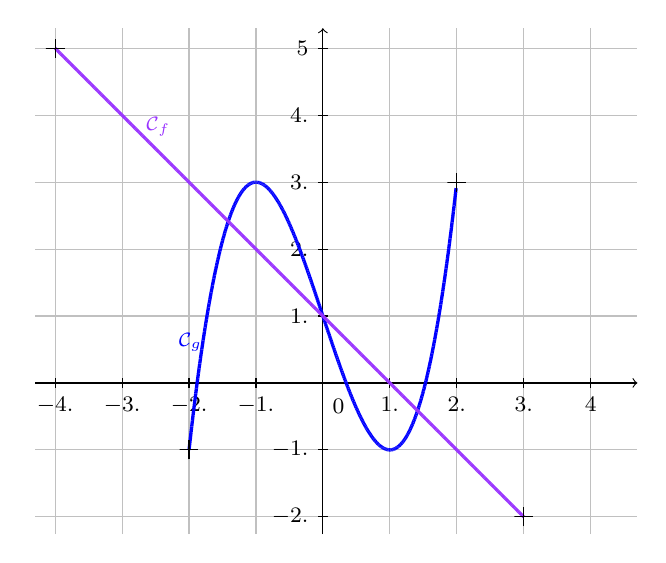
\begin{tikzpicture}[scale=0.85][line cap=round,line join=round,>=triangle 45,x=1.0cm,y=1.0cm]
\draw [color=cqcqcq,, xstep=1.0cm,ystep=1.0cm] (-4.3,-2.26) grid (4.7,5.3);
\draw[->,color=black] (-4.3,0.) -- (4.7,0.);
\foreach \x in {-4.,-3.,-2.,-1.,1.,2.,3.,4}
\draw[shift={(\x,0)},color=black] (0pt,2pt) -- (0pt,-2pt) node[below] {\footnotesize $\x$};
\draw[->,color=black] (0.,-2.26) -- (0.,5.3);
\foreach \y in {-2.,-1.,1.,2.,3.,4.,5}
\draw[shift={(0,\y)},color=black] (2pt,0pt) -- (-2pt,0pt) node[left] {\footnotesize $\y$};
\draw[color=black] (0pt,-10pt) node[right] {\footnotesize $0$};
\clip(-4.3,-2.26) rectangle (4.7,5.3);
\draw[line width=1.2pt,color=qqqqff] (-2.0000000000000027,-1.000000000000024) -- (-2.0000000000000027,-1.000000000000024);
\draw[line width=1.2pt,color=qqqqff] (-2.0000000000000027,-1.000000000000024) -- (-1.9900000002575027,-0.910599002286701);
\draw[line width=1.2pt,color=qqqqff] (-1.9900000002575027,-0.910599002286701) -- (-1.9800000005150027,-0.8223920045120415);
\draw[line width=1.2pt,color=qqqqff] (-1.9800000005150027,-0.8223920045120415) -- (-1.9700000007725027,-0.7353730066765092);
\draw[line width=1.2pt,color=qqqqff] (-1.9700000007725027,-0.7353730066765092) -- (-1.9600000010300027,-0.6495360087805672);
\draw[line width=1.2pt,color=qqqqff] (-1.9600000010300027,-0.6495360087805672) -- (-1.9500000012875027,-0.5648750108246792);
\draw[line width=1.2pt,color=qqqqff] (-1.9500000012875027,-0.5648750108246792) -- (-1.9400000015450027,-0.48138401280930865);
\draw[line width=1.2pt,color=qqqqff] (-1.9400000015450027,-0.48138401280930865) -- (-1.9300000018025028,-0.3990570147349193);
\draw[line width=1.2pt,color=qqqqff] (-1.9300000018025028,-0.3990570147349193) -- (-1.9200000020600028,-0.3178880166019743);
\draw[line width=1.2pt,color=qqqqff] (-1.9200000020600028,-0.3178880166019743) -- (-1.9100000023175028,-0.23787101841093727);
\draw[line width=1.2pt,color=qqqqff] (-1.9100000023175028,-0.23787101841093727) -- (-1.9000000025750028,-0.15900002016227177);
\draw[line width=1.2pt,color=qqqqff] (-1.9000000025750028,-0.15900002016227177) -- (-1.8900000028325028,-0.08126902185644147);
\draw[line width=1.2pt,color=qqqqff] (-1.8900000028325028,-0.08126902185644147) -- (-1.8800000030900028,-0.004672023493909383);
\draw[line width=1.2pt,color=qqqqff] (-1.8800000030900028,-0.004672023493909383) -- (-1.8700000033475028,0.07079697492486048);
\draw[line width=1.2pt,color=qqqqff] (-1.8700000033475028,0.07079697492486048) -- (-1.8600000036050028,0.1451439733994051);
\draw[line width=1.2pt,color=qqqqff] (-1.8600000036050028,0.1451439733994051) -- (-1.8500000038625029,0.21837497192926048);
\draw[line width=1.2pt,color=qqqqff] (-1.8500000038625029,0.21837497192926048) -- (-1.8400000041200029,0.29049597051396336);
\draw[line width=1.2pt,color=qqqqff] (-1.8400000041200029,0.29049597051396336) -- (-1.8300000043775029,0.36151296915305053);
\draw[line width=1.2pt,color=qqqqff] (-1.8300000043775029,0.36151296915305053) -- (-1.8200000046350029,0.43143196784605786);
\draw[line width=1.2pt,color=qqqqff] (-1.8200000046350029,0.43143196784605786) -- (-1.810000004892503,0.5002589665925223);
\draw[line width=1.2pt,color=qqqqff] (-1.810000004892503,0.5002589665925223) -- (-1.800000005150003,0.5679999653919803);
\draw[line width=1.2pt,color=qqqqff] (-1.800000005150003,0.5679999653919803) -- (-1.790000005407503,0.6346609642439682);
\draw[line width=1.2pt,color=qqqqff] (-1.790000005407503,0.6346609642439682) -- (-1.780000005665003,0.7002479631480227);
\draw[line width=1.2pt,color=qqqqff] (-1.780000005665003,0.7002479631480227) -- (-1.770000005922503,0.7647669621036801);
\draw[line width=1.2pt,color=qqqqff] (-1.770000005922503,0.7647669621036801) -- (-1.760000006180003,0.8282239611104771);
\draw[line width=1.2pt,color=qqqqff] (-1.760000006180003,0.8282239611104771) -- (-1.750000006437503,0.8906249601679501);
\draw[line width=1.2pt,color=qqqqff] (-1.750000006437503,0.8906249601679501) -- (-1.740000006695003,0.9519759592756356);
\draw[line width=1.2pt,color=qqqqff] (-1.740000006695003,0.9519759592756356) -- (-1.730000006952503,1.0122829584330701);
\draw[line width=1.2pt,color=qqqqff] (-1.730000006952503,1.0122829584330701) -- (-1.720000007210003,1.07155195763979);
\draw[line width=1.2pt,color=qqqqff] (-1.720000007210003,1.07155195763979) -- (-1.710000007467503,1.1297889568953319);
\draw[line width=1.2pt,color=qqqqff] (-1.710000007467503,1.1297889568953319) -- (-1.700000007725003,1.1869999561992324);
\draw[line width=1.2pt,color=qqqqff] (-1.700000007725003,1.1869999561992324) -- (-1.690000007982503,1.2431909555510279);
\draw[line width=1.2pt,color=qqqqff] (-1.690000007982503,1.2431909555510279) -- (-1.680000008240003,1.2983679549502551);
\draw[line width=1.2pt,color=qqqqff] (-1.680000008240003,1.2983679549502551) -- (-1.670000008497503,1.35253695439645);
\draw[line width=1.2pt,color=qqqqff] (-1.670000008497503,1.35253695439645) -- (-1.660000008755003,1.4057039538891494);
\draw[line width=1.2pt,color=qqqqff] (-1.660000008755003,1.4057039538891494) -- (-1.650000009012503,1.4578749534278899);
\draw[line width=1.2pt,color=qqqqff] (-1.650000009012503,1.4578749534278899) -- (-1.6400000092700031,1.5090559530122079);
\draw[line width=1.2pt,color=qqqqff] (-1.6400000092700031,1.5090559530122079) -- (-1.6300000095275031,1.5592529526416397);
\draw[line width=1.2pt,color=qqqqff] (-1.6300000095275031,1.5592529526416397) -- (-1.6200000097850031,1.608471952315722);
\draw[line width=1.2pt,color=qqqqff] (-1.6200000097850031,1.608471952315722) -- (-1.6100000100425031,1.6567189520339918);
\draw[line width=1.2pt,color=qqqqff] (-1.6100000100425031,1.6567189520339918) -- (-1.6000000103000032,1.7039999517959847);
\draw[line width=1.2pt,color=qqqqff] (-1.6000000103000032,1.7039999517959847) -- (-1.5900000105575032,1.7503209516012377);
\draw[line width=1.2pt,color=qqqqff] (-1.5900000105575032,1.7503209516012377) -- (-1.5800000108150032,1.7956879514492874);
\draw[line width=1.2pt,color=qqqqff] (-1.5800000108150032,1.7956879514492874) -- (-1.5700000110725032,1.8401069513396697);
\draw[line width=1.2pt,color=qqqqff] (-1.5700000110725032,1.8401069513396697) -- (-1.5600000113300032,1.883583951271922);
\draw[line width=1.2pt,color=qqqqff] (-1.5600000113300032,1.883583951271922) -- (-1.5500000115875032,1.9261249512455798);
\draw[line width=1.2pt,color=qqqqff] (-1.5500000115875032,1.9261249512455798) -- (-1.5400000118450032,1.9677359512601797);
\draw[line width=1.2pt,color=qqqqff] (-1.5400000118450032,1.9677359512601797) -- (-1.5300000121025032,2.0084229513152594);
\draw[line width=1.2pt,color=qqqqff] (-1.5300000121025032,2.0084229513152594) -- (-1.5200000123600033,2.048191951410354);
\draw[line width=1.2pt,color=qqqqff] (-1.5200000123600033,2.048191951410354) -- (-1.5100000126175033,2.0870489515450013);
\draw[line width=1.2pt,color=qqqqff] (-1.5100000126175033,2.0870489515450013) -- (-1.5000000128750033,2.124999951718737);
\draw[line width=1.2pt,color=qqqqff] (-1.5000000128750033,2.124999951718737) -- (-1.4900000131325033,2.1620509519310973);
\draw[line width=1.2pt,color=qqqqff] (-1.4900000131325033,2.1620509519310973) -- (-1.4800000133900033,2.1982079521816194);
\draw[line width=1.2pt,color=qqqqff] (-1.4800000133900033,2.1982079521816194) -- (-1.4700000136475033,2.2334769524698395);
\draw[line width=1.2pt,color=qqqqff] (-1.4700000136475033,2.2334769524698395) -- (-1.4600000139050033,2.267863952795294);
\draw[line width=1.2pt,color=qqqqff] (-1.4600000139050033,2.267863952795294) -- (-1.4500000141625033,2.3013749531575196);
\draw[line width=1.2pt,color=qqqqff] (-1.4500000141625033,2.3013749531575196) -- (-1.4400000144200034,2.3340159535560523);
\draw[line width=1.2pt,color=qqqqff] (-1.4400000144200034,2.3340159535560523) -- (-1.4300000146775034,2.365792953990429);
\draw[line width=1.2pt,color=qqqqff] (-1.4300000146775034,2.365792953990429) -- (-1.4200000149350034,2.3967119544601867);
\draw[line width=1.2pt,color=qqqqff] (-1.4200000149350034,2.3967119544601867) -- (-1.4100000151925034,2.4267789549648615);
\draw[line width=1.2pt,color=qqqqff] (-1.4100000151925034,2.4267789549648615) -- (-1.4000000154500034,2.455999955503989);
\draw[line width=1.2pt,color=qqqqff] (-1.4000000154500034,2.455999955503989) -- (-1.3900000157075034,2.484380956077107);
\draw[line width=1.2pt,color=qqqqff] (-1.3900000157075034,2.484380956077107) -- (-1.3800000159650034,2.511927956683752);
\draw[line width=1.2pt,color=qqqqff] (-1.3800000159650034,2.511927956683752) -- (-1.3700000162225034,2.538646957323459);
\draw[line width=1.2pt,color=qqqqff] (-1.3700000162225034,2.538646957323459) -- (-1.3600000164800035,2.564543957995766);
\draw[line width=1.2pt,color=qqqqff] (-1.3600000164800035,2.564543957995766) -- (-1.3500000167375035,2.5896249587002087);
\draw[line width=1.2pt,color=qqqqff] (-1.3500000167375035,2.5896249587002087) -- (-1.3400000169950035,2.6138959594363245);
\draw[line width=1.2pt,color=qqqqff] (-1.3400000169950035,2.6138959594363245) -- (-1.3300000172525035,2.637362960203649);
\draw[line width=1.2pt,color=qqqqff] (-1.3300000172525035,2.637362960203649) -- (-1.3200000175100035,2.6600319610017187);
\draw[line width=1.2pt,color=qqqqff] (-1.3200000175100035,2.6600319610017187) -- (-1.3100000177675035,2.6819089618300707);
\draw[line width=1.2pt,color=qqqqff] (-1.3100000177675035,2.6819089618300707) -- (-1.3000000180250035,2.7029999626882413);
\draw[line width=1.2pt,color=qqqqff] (-1.3000000180250035,2.7029999626882413) -- (-1.2900000182825035,2.723310963575767);
\draw[line width=1.2pt,color=qqqqff] (-1.2900000182825035,2.723310963575767) -- (-1.2800000185400036,2.742847964492184);
\draw[line width=1.2pt,color=qqqqff] (-1.2800000185400036,2.742847964492184) -- (-1.2700000187975036,2.761616965437029);
\draw[line width=1.2pt,color=qqqqff] (-1.2700000187975036,2.761616965437029) -- (-1.2600000190550036,2.7796239664098383);
\draw[line width=1.2pt,color=qqqqff] (-1.2600000190550036,2.7796239664098383) -- (-1.2500000193125036,2.7968749674101483);
\draw[line width=1.2pt,color=qqqqff] (-1.2500000193125036,2.7968749674101483) -- (-1.2400000195700036,2.813375968437497);
\draw[line width=1.2pt,color=qqqqff] (-1.2400000195700036,2.813375968437497) -- (-1.2300000198275036,2.8291329694914187);
\draw[line width=1.2pt,color=qqqqff] (-1.2300000198275036,2.8291329694914187) -- (-1.2200000200850036,2.8441519705714513);
\draw[line width=1.2pt,color=qqqqff] (-1.2200000200850036,2.8441519705714513) -- (-1.2100000203425036,2.858438971677131);
\draw[line width=1.2pt,color=qqqqff] (-1.2100000203425036,2.858438971677131) -- (-1.2000000206000037,2.8719999728079935);
\draw[line width=1.2pt,color=qqqqff] (-1.2000000206000037,2.8719999728079935) -- (-1.1900000208575037,2.884840973963577);
\draw[line width=1.2pt,color=qqqqff] (-1.1900000208575037,2.884840973963577) -- (-1.1800000211150037,2.8969679751434163);
\draw[line width=1.2pt,color=qqqqff] (-1.1800000211150037,2.8969679751434163) -- (-1.1700000213725037,2.9083869763470482);
\draw[line width=1.2pt,color=qqqqff] (-1.1700000213725037,2.9083869763470482) -- (-1.1600000216300037,2.919103977574011);
\draw[line width=1.2pt,color=qqqqff] (-1.1600000216300037,2.919103977574011) -- (-1.1500000218875037,2.9291249788238383);
\draw[line width=1.2pt,color=qqqqff] (-1.1500000218875037,2.9291249788238383) -- (-1.1400000221450037,2.938455980096069);
\draw[line width=1.2pt,color=qqqqff] (-1.1400000221450037,2.938455980096069) -- (-1.1300000224025037,2.9471029813902385);
\draw[line width=1.2pt,color=qqqqff] (-1.1300000224025037,2.9471029813902385) -- (-1.1200000226600038,2.955071982705883);
\draw[line width=1.2pt,color=qqqqff] (-1.1200000226600038,2.955071982705883) -- (-1.1100000229175038,2.9623689840425405);
\draw[line width=1.2pt,color=qqqqff] (-1.1100000229175038,2.9623689840425405) -- (-1.1000000231750038,2.968999985399746);
\draw[line width=1.2pt,color=qqqqff] (-1.1000000231750038,2.968999985399746) -- (-1.0900000234325038,2.974970986777037);
\draw[line width=1.2pt,color=qqqqff] (-1.0900000234325038,2.974970986777037) -- (-1.0800000236900038,2.980287988173948);
\draw[line width=1.2pt,color=qqqqff] (-1.0800000236900038,2.980287988173948) -- (-1.0700000239475038,2.984956989590018);
\draw[line width=1.2pt,color=qqqqff] (-1.0700000239475038,2.984956989590018) -- (-1.0600000242050038,2.9889839910247824);
\draw[line width=1.2pt,color=qqqqff] (-1.0600000242050038,2.9889839910247824) -- (-1.0500000244625038,2.992374992477778);
\draw[line width=1.2pt,color=qqqqff] (-1.0500000244625038,2.992374992477778) -- (-1.0400000247200039,2.995135993948541);
\draw[line width=1.2pt,color=qqqqff] (-1.0400000247200039,2.995135993948541) -- (-1.0300000249775039,2.997272995436608);
\draw[line width=1.2pt,color=qqqqff] (-1.0300000249775039,2.997272995436608) -- (-1.0200000252350039,2.9987919969415153);
\draw[line width=1.2pt,color=qqqqff] (-1.0200000252350039,2.9987919969415153) -- (-1.010000025492504,2.9996989984628);
\draw[line width=1.2pt,color=qqqqff] (-1.010000025492504,2.9996989984628) -- (-1.000000025750004,2.9999999999999982);
\draw[line width=1.2pt,color=qqqqff] (-1.000000025750004,2.9999999999999982) -- (-0.9900000260075039,2.999701001552646);
\draw[line width=1.2pt,color=qqqqff] (-0.9900000260075039,2.999701001552646) -- (-0.9800000262650039,2.9988080031202804);
\draw[line width=1.2pt,color=qqqqff] (-0.9800000262650039,2.9988080031202804) -- (-0.9700000265225039,2.997327004702438);
\draw[line width=1.2pt,color=qqqqff] (-0.9700000265225039,2.997327004702438) -- (-0.960000026780004,2.9952640062986546);
\draw[line width=1.2pt,color=qqqqff] (-0.960000026780004,2.9952640062986546) -- (-0.950000027037504,2.992625007908468);
\draw[line width=1.2pt,color=qqqqff] (-0.950000027037504,2.992625007908468) -- (-0.940000027295004,2.9894160095314133);
\draw[line width=1.2pt,color=qqqqff] (-0.940000027295004,2.9894160095314133) -- (-0.930000027552504,2.985643011167028);
\draw[line width=1.2pt,color=qqqqff] (-0.930000027552504,2.985643011167028) -- (-0.920000027810004,2.9813120128148474);
\draw[line width=1.2pt,color=qqqqff] (-0.920000027810004,2.9813120128148474) -- (-0.910000028067504,2.9764290144744097);
\draw[line width=1.2pt,color=qqqqff] (-0.910000028067504,2.9764290144744097) -- (-0.900000028325004,2.9710000161452506);
\draw[line width=1.2pt,color=qqqqff] (-0.900000028325004,2.9710000161452506) -- (-0.890000028582504,2.9650310178269055);
\draw[line width=1.2pt,color=qqqqff] (-0.890000028582504,2.9650310178269055) -- (-0.8800000288400041,2.9585280195189125);
\draw[line width=1.2pt,color=qqqqff] (-0.8800000288400041,2.9585280195189125) -- (-0.8700000290975041,2.951497021220807);
\draw[line width=1.2pt,color=qqqqff] (-0.8700000290975041,2.951497021220807) -- (-0.8600000293550041,2.943944022932127);
\draw[line width=1.2pt,color=qqqqff] (-0.8600000293550041,2.943944022932127) -- (-0.8500000296125041,2.9358750246524075);
\draw[line width=1.2pt,color=qqqqff] (-0.8500000296125041,2.9358750246524075) -- (-0.8400000298700041,2.9272960263811854);
\draw[line width=1.2pt,color=qqqqff] (-0.8400000298700041,2.9272960263811854) -- (-0.8300000301275041,2.9182130281179974);
\draw[line width=1.2pt,color=qqqqff] (-0.8300000301275041,2.9182130281179974) -- (-0.8200000303850041,2.9086320298623796);
\draw[line width=1.2pt,color=qqqqff] (-0.8200000303850041,2.9086320298623796) -- (-0.8100000306425041,2.898559031613869);
\draw[line width=1.2pt,color=qqqqff] (-0.8100000306425041,2.898559031613869) -- (-0.8000000309000042,2.8880000333720024);
\draw[line width=1.2pt,color=qqqqff] (-0.8000000309000042,2.8880000333720024) -- (-0.7900000311575042,2.8769610351363153);
\draw[line width=1.2pt,color=qqqqff] (-0.7900000311575042,2.8769610351363153) -- (-0.7800000314150042,2.8654480369063444);
\draw[line width=1.2pt,color=qqqqff] (-0.7800000314150042,2.8654480369063444) -- (-0.7700000316725042,2.853467038681627);
\draw[line width=1.2pt,color=qqqqff] (-0.7700000316725042,2.853467038681627) -- (-0.7600000319300042,2.841024040461699);
\draw[line width=1.2pt,color=qqqqff] (-0.7600000319300042,2.841024040461699) -- (-0.7500000321875042,2.828125042246097);
\draw[line width=1.2pt,color=qqqqff] (-0.7500000321875042,2.828125042246097) -- (-0.7400000324450042,2.8147760440343577);
\draw[line width=1.2pt,color=qqqqff] (-0.7400000324450042,2.8147760440343577) -- (-0.7300000327025042,2.8009830458260168);
\draw[line width=1.2pt,color=qqqqff] (-0.7300000327025042,2.8009830458260168) -- (-0.7200000329600043,2.786752047620612);
\draw[line width=1.2pt,color=qqqqff] (-0.7200000329600043,2.786752047620612) -- (-0.7100000332175043,2.7720890494176786);
\draw[line width=1.2pt,color=qqqqff] (-0.7100000332175043,2.7720890494176786) -- (-0.7000000334750043,2.7570000512167545);
\draw[line width=1.2pt,color=qqqqff] (-0.7000000334750043,2.7570000512167545) -- (-0.6900000337325043,2.741491053017375);
\draw[line width=1.2pt,color=qqqqff] (-0.6900000337325043,2.741491053017375) -- (-0.6800000339900043,2.7255680548190764);
\draw[line width=1.2pt,color=qqqqff] (-0.6800000339900043,2.7255680548190764) -- (-0.6700000342475043,2.7092370566213964);
\draw[line width=1.2pt,color=qqqqff] (-0.6700000342475043,2.7092370566213964) -- (-0.6600000345050043,2.692504058423871);
\draw[line width=1.2pt,color=qqqqff] (-0.6600000345050043,2.692504058423871) -- (-0.6500000347625043,2.6753750602260364);
\draw[line width=1.2pt,color=qqqqff] (-0.6500000347625043,2.6753750602260364) -- (-0.6400000350200044,2.6578560620274296);
\draw[line width=1.2pt,color=qqqqff] (-0.6400000350200044,2.6578560620274296) -- (-0.6300000352775044,2.6399530638275865);
\draw[line width=1.2pt,color=qqqqff] (-0.6300000352775044,2.6399530638275865) -- (-0.6200000355350044,2.6216720656260435);
\draw[line width=1.2pt,color=qqqqff] (-0.6200000355350044,2.6216720656260435) -- (-0.6100000357925044,2.603019067422338);
\draw[line width=1.2pt,color=qqqqff] (-0.6100000357925044,2.603019067422338) -- (-0.6000000360500044,2.584000069216006);
\draw[line width=1.2pt,color=qqqqff] (-0.6000000360500044,2.584000069216006) -- (-0.5900000363075044,2.564621071006584);
\draw[line width=1.2pt,color=qqqqff] (-0.5900000363075044,2.564621071006584) -- (-0.5800000365650044,2.5448880727936087);
\draw[line width=1.2pt,color=qqqqff] (-0.5800000365650044,2.5448880727936087) -- (-0.5700000368225044,2.524807074576616);
\draw[line width=1.2pt,color=qqqqff] (-0.5700000368225044,2.524807074576616) -- (-0.5600000370800045,2.504384076355143);
\draw[line width=1.2pt,color=qqqqff] (-0.5600000370800045,2.504384076355143) -- (-0.5500000373375045,2.483625078128726);
\draw[line width=1.2pt,color=qqqqff] (-0.5500000373375045,2.483625078128726) -- (-0.5400000375950045,2.4625360798969016);
\draw[line width=1.2pt,color=qqqqff] (-0.5400000375950045,2.4625360798969016) -- (-0.5300000378525045,2.4411230816592058);
\draw[line width=1.2pt,color=qqqqff] (-0.5300000378525045,2.4411230816592058) -- (-0.5200000381100045,2.4193920834151754);
\draw[line width=1.2pt,color=qqqqff] (-0.5200000381100045,2.4193920834151754) -- (-0.5100000383675045,2.3973490851643477);
\draw[line width=1.2pt,color=qqqqff] (-0.5100000383675045,2.3973490851643477) -- (-0.5000000386250045,2.3750000869062577);
\draw[line width=1.2pt,color=qqqqff] (-0.5000000386250045,2.3750000869062577) -- (-0.4900000388825045,2.3523510886404435);
\draw[line width=1.2pt,color=qqqqff] (-0.4900000388825045,2.3523510886404435) -- (-0.48000003914000444,2.32940809036644);
\draw[line width=1.2pt,color=qqqqff] (-0.48000003914000444,2.32940809036644) -- (-0.4700000393975044,2.3061770920837845);
\draw[line width=1.2pt,color=qqqqff] (-0.4700000393975044,2.3061770920837845) -- (-0.46000003965500436,2.282664093792014);
\draw[line width=1.2pt,color=qqqqff] (-0.46000003965500436,2.282664093792014) -- (-0.4500000399125043,2.2588750954906645);
\draw[line width=1.2pt,color=qqqqff] (-0.4500000399125043,2.2588750954906645) -- (-0.44000004017000427,2.234816097179272);
\draw[line width=1.2pt,color=qqqqff] (-0.44000004017000427,2.234816097179272) -- (-0.4300000404275042,2.210493098857374);
\draw[line width=1.2pt,color=qqqqff] (-0.4300000404275042,2.210493098857374) -- (-0.4200000406850042,2.1859121005245066);
\draw[line width=1.2pt,color=qqqqff] (-0.4200000406850042,2.1859121005245066) -- (-0.41000004094250414,2.1610791021802056);
\draw[line width=1.2pt,color=qqqqff] (-0.41000004094250414,2.1610791021802056) -- (-0.4000000412000041,2.1360001038240086);
\draw[line width=1.2pt,color=qqqqff] (-0.4000000412000041,2.1360001038240086) -- (-0.39000004145750405,2.110681105455451);
\draw[line width=1.2pt,color=qqqqff] (-0.39000004145750405,2.110681105455451) -- (-0.380000041715004,2.0851281070740706);
\draw[line width=1.2pt,color=qqqqff] (-0.380000041715004,2.0851281070740706) -- (-0.37000004197250397,2.0593471086794026);
\draw[line width=1.2pt,color=qqqqff] (-0.37000004197250397,2.0593471086794026) -- (-0.3600000422300039,2.0333441102709844);
\draw[line width=1.2pt,color=qqqqff] (-0.3600000422300039,2.0333441102709844) -- (-0.3500000424875039,2.0071251118483517);
\draw[line width=1.2pt,color=qqqqff] (-0.3500000424875039,2.0071251118483517) -- (-0.34000004274500384,1.9806961134110423);
\draw[line width=1.2pt,color=qqqqff] (-0.34000004274500384,1.9806961134110423) -- (-0.3300000430025038,1.9540631149585916);
\draw[line width=1.2pt,color=qqqqff] (-0.3300000430025038,1.9540631149585916) -- (-0.32000004326000375,1.9272321164905364);
\draw[line width=1.2pt,color=qqqqff] (-0.32000004326000375,1.9272321164905364) -- (-0.3100000435175037,1.900209118006413);
\draw[line width=1.2pt,color=qqqqff] (-0.3100000435175037,1.900209118006413) -- (-0.30000004377500367,1.873000119505758);
\draw[line width=1.2pt,color=qqqqff] (-0.30000004377500367,1.873000119505758) -- (-0.2900000440325036,1.8456111209881083);
\draw[line width=1.2pt,color=qqqqff] (-0.2900000440325036,1.8456111209881083) -- (-0.2800000442900036,1.8180481224529998);
\draw[line width=1.2pt,color=qqqqff] (-0.2800000442900036,1.8180481224529998) -- (-0.27000004454750354,1.7903171238999698);
\draw[line width=1.2pt,color=qqqqff] (-0.27000004454750354,1.7903171238999698) -- (-0.2600000448050035,1.7624241253285544);
\draw[line width=1.2pt,color=qqqqff] (-0.2600000448050035,1.7624241253285544) -- (-0.25000004506250345,1.7343751267382896);
\draw[line width=1.2pt,color=qqqqff] (-0.25000004506250345,1.7343751267382896) -- (-0.24000004532000344,1.7061761281287122);
\draw[line width=1.2pt,color=qqqqff] (-0.24000004532000344,1.7061761281287122) -- (-0.23000004557750342,1.6778331294993594);
\draw[line width=1.2pt,color=qqqqff] (-0.23000004557750342,1.6778331294993594) -- (-0.2200000458350034,1.649352130849766);
\draw[line width=1.2pt,color=qqqqff] (-0.2200000458350034,1.649352130849766) -- (-0.2100000460925034,1.6207391321794704);
\draw[line width=1.2pt,color=qqqqff] (-0.2100000460925034,1.6207391321794704) -- (-0.20000004635000337,1.5920001334880083);
\draw[line width=1.2pt,color=qqqqff] (-0.20000004635000337,1.5920001334880083) -- (-0.19000004660750336,1.5631411347749165);
\draw[line width=1.2pt,color=qqqqff] (-0.19000004660750336,1.5631411347749165) -- (-0.18000004686500334,1.5341681360397303);
\draw[line width=1.2pt,color=qqqqff] (-0.18000004686500334,1.5341681360397303) -- (-0.17000004712250333,1.5050871372819876);
\draw[line width=1.2pt,color=qqqqff] (-0.17000004712250333,1.5050871372819876) -- (-0.1600000473800033,1.475904138501225);
\draw[line width=1.2pt,color=qqqqff] (-0.1600000473800033,1.475904138501225) -- (-0.1500000476375033,1.4466251396969771);
\draw[line width=1.2pt,color=qqqqff] (-0.1500000476375033,1.4466251396969771) -- (-0.14000004789500328,1.4172561408687825);
\draw[line width=1.2pt,color=qqqqff] (-0.14000004789500328,1.4172561408687825) -- (-0.13000004815250327,1.387803142016177);
\draw[line width=1.2pt,color=qqqqff] (-0.13000004815250327,1.387803142016177) -- (-0.12000004841000325,1.3582721431386968);
\draw[line width=1.2pt,color=qqqqff] (-0.12000004841000325,1.3582721431386968) -- (-0.11000004866750324,1.328669144235879);
\draw[line width=1.2pt,color=qqqqff] (-0.11000004866750324,1.328669144235879) -- (-0.10000004892500322,1.299000145307259);
\draw[line width=1.2pt,color=qqqqff] (-0.10000004892500322,1.299000145307259) -- (-0.0900000491825032,1.2692711463523745);
\draw[line width=1.2pt,color=qqqqff] (-0.0900000491825032,1.2692711463523745) -- (-0.08000004944000319,1.239488147370761);
\draw[line width=1.2pt,color=qqqqff] (-0.08000004944000319,1.239488147370761) -- (-0.07000004969750317,1.209657148361956);
\draw[line width=1.2pt,color=qqqqff] (-0.07000004969750317,1.209657148361956) -- (-0.06000004995500316,1.1797841493254948);
\draw[line width=1.2pt,color=qqqqff] (-0.06000004995500316,1.1797841493254948) -- (-0.050000050212503144,1.1498751502609155);
\draw[line width=1.2pt,color=qqqqff] (-0.050000050212503144,1.1498751502609155) -- (-0.04000005047000313,1.119936151167753);
\draw[line width=1.2pt,color=qqqqff] (-0.04000005047000313,1.119936151167753) -- (-0.030000050727503114,1.0899731520455451);
\draw[line width=1.2pt,color=qqqqff] (-0.030000050727503114,1.0899731520455451) -- (-0.0200000509850031,1.0599921528938272);
\draw[line width=1.2pt,color=qqqqff] (-0.0200000509850031,1.0599921528938272) -- (-0.010000051242503081,1.0299991537121365);
\draw[line width=1.2pt,color=qqqqff] (-0.010000051242503081,1.0299991537121365) -- (0.0,1.0000001545000097);
\draw[line width=1.2pt,color=qqqqff] (0.0,1.0000001545000097) -- (0.009999999742500017,0.9700010007724227);
\draw[line width=1.2pt,color=qqqqff] (0.009999999742500017,0.9700010007724227) -- (0.019999999485000034,0.9400080015443817);
\draw[line width=1.2pt,color=qqqqff] (0.019999999485000034,0.9400080015443817) -- (0.029999999227500053,0.9100270023154138);
\draw[line width=1.2pt,color=qqqqff] (0.029999999227500053,0.9100270023154138) -- (0.03999999897000007,0.8800640030850557);
\draw[line width=1.2pt,color=qqqqff] (0.03999999897000007,0.8800640030850557) -- (0.049999998712500084,0.8501250038528436);
\draw[line width=1.2pt,color=qqqqff] (0.049999998712500084,0.8501250038528436) -- (0.0599999984550001,0.8202160046183133);
\draw[line width=1.2pt,color=qqqqff] (0.0599999984550001,0.8202160046183133) -- (0.06999999819750012,0.7903430053810026);
\draw[line width=1.2pt,color=qqqqff] (0.06999999819750012,0.7903430053810026) -- (0.07999999794000014,0.760512006140448);
\draw[line width=1.2pt,color=qqqqff] (0.07999999794000014,0.760512006140448) -- (0.08999999768250015,0.7307290068961847);
\draw[line width=1.2pt,color=qqqqff] (0.08999999768250015,0.7307290068961847) -- (0.09999999742500017,0.7010000076477496);
\draw[line width=1.2pt,color=qqqqff] (0.09999999742500017,0.7010000076477496) -- (0.10999999716750018,0.6713310083946797);
\draw[line width=1.2pt,color=qqqqff] (0.10999999716750018,0.6713310083946797) -- (0.1199999969100002,0.6417280091365116);
\draw[line width=1.2pt,color=qqqqff] (0.1199999969100002,0.6417280091365116) -- (0.12999999665250023,0.6121970098727809);
\draw[line width=1.2pt,color=qqqqff] (0.12999999665250023,0.6121970098727809) -- (0.13999999639500024,0.582744010603025);
\draw[line width=1.2pt,color=qqqqff] (0.13999999639500024,0.582744010603025) -- (0.14999999613750026,0.5533750113267806);
\draw[line width=1.2pt,color=qqqqff] (0.14999999613750026,0.5533750113267806) -- (0.15999999588000027,0.5240960120435834);
\draw[line width=1.2pt,color=qqqqff] (0.15999999588000027,0.5240960120435834) -- (0.1699999956225003,0.49491301275297017);
\draw[line width=1.2pt,color=qqqqff] (0.1699999956225003,0.49491301275297017) -- (0.1799999953650003,0.4658320134544771);
\draw[line width=1.2pt,color=qqqqff] (0.1799999953650003,0.4658320134544771) -- (0.18999999510750032,0.4368590141476414);
\draw[line width=1.2pt,color=qqqqff] (0.18999999510750032,0.4368590141476414) -- (0.19999999485000033,0.4080000148319991);
\draw[line width=1.2pt,color=qqqqff] (0.19999999485000033,0.4080000148319991) -- (0.20999999459250035,0.3792610155070866);
\draw[line width=1.2pt,color=qqqqff] (0.20999999459250035,0.3792610155070866) -- (0.21999999433500037,0.3506480161724408);
\draw[line width=1.2pt,color=qqqqff] (0.21999999433500037,0.3506480161724408) -- (0.22999999407750038,0.3221670168275983);
\draw[line width=1.2pt,color=qqqqff] (0.22999999407750038,0.3221670168275983) -- (0.2399999938200004,0.29382401747209497);
\draw[line width=1.2pt,color=qqqqff] (0.2399999938200004,0.29382401747209497) -- (0.2499999935625004,0.2656250181054678);
\draw[line width=1.2pt,color=qqqqff] (0.2499999935625004,0.2656250181054678) -- (0.25999999330500045,0.23757601872725287);
\draw[line width=1.2pt,color=qqqqff] (0.25999999330500045,0.23757601872725287) -- (0.2699999930475005,0.20968301933698674);
\draw[line width=1.2pt,color=qqqqff] (0.2699999930475005,0.20968301933698674) -- (0.27999999279000054,0.1819520199342064);
\draw[line width=1.2pt,color=qqqqff] (0.27999999279000054,0.1819520199342064) -- (0.2899999925325006,0.15438902051844838);
\draw[line width=1.2pt,color=qqqqff] (0.2899999925325006,0.15438902051844838) -- (0.2999999922750006,0.12700002108924835);
\draw[line width=1.2pt,color=qqqqff] (0.2999999922750006,0.12700002108924835) -- (0.30999999201750067,0.09979102164614329);
\draw[line width=1.2pt,color=qqqqff] (0.30999999201750067,0.09979102164614329) -- (0.3199999917600007,0.07276802218867018);
\draw[line width=1.2pt,color=qqqqff] (0.3199999917600007,0.07276802218867018) -- (0.32999999150250076,0.04593702271636513);
\draw[line width=1.2pt,color=qqqqff] (0.32999999150250076,0.04593702271636513) -- (0.3399999912450008,0.01930402322876401);
\draw[line width=1.2pt,color=qqqqff] (0.3399999912450008,0.01930402322876401) -- (0.34999999098750084,-0.007124976274596073);
\draw[line width=1.2pt,color=qqqqff] (0.34999999098750084,-0.007124976274596073) -- (0.3599999907300009,-0.03334397579417814);
\draw[line width=1.2pt,color=qqqqff] (0.3599999907300009,-0.03334397579417814) -- (0.36999999047250093,-0.059346975330446416);
\draw[line width=1.2pt,color=qqqqff] (0.36999999047250093,-0.059346975330446416) -- (0.37999999021500097,-0.08512797488386437);
\draw[line width=1.2pt,color=qqqqff] (0.37999999021500097,-0.08512797488386437) -- (0.389999989957501,-0.11068097445489544);
\draw[line width=1.2pt,color=qqqqff] (0.389999989957501,-0.11068097445489544) -- (0.39999998970000106,-0.13599997404400244);
\draw[line width=1.2pt,color=qqqqff] (0.39999998970000106,-0.13599997404400244) -- (0.4099999894425011,-0.16107897365164958);
\draw[line width=1.2pt,color=qqqqff] (0.4099999894425011,-0.16107897365164958) -- (0.41999998918500114,-0.18591197327830056);
\draw[line width=1.2pt,color=qqqqff] (0.41999998918500114,-0.18591197327830056) -- (0.4299999889275012,-0.2104929729244186);
\draw[line width=1.2pt,color=qqqqff] (0.4299999889275012,-0.2104929729244186) -- (0.43999998867000123,-0.23481597259046683);
\draw[line width=1.2pt,color=qqqqff] (0.43999998867000123,-0.23481597259046683) -- (0.4499999884125013,-0.25887497227690903);
\draw[line width=1.2pt,color=qqqqff] (0.4499999884125013,-0.25887497227690903) -- (0.4599999881550013,-0.2826639719842089);
\draw[line width=1.2pt,color=qqqqff] (0.4599999881550013,-0.2826639719842089) -- (0.46999998789750136,-0.30617697171283);
\draw[line width=1.2pt,color=qqqqff] (0.46999998789750136,-0.30617697171283) -- (0.4799999876400014,-0.3294079714632351);
\draw[line width=1.2pt,color=qqqqff] (0.4799999876400014,-0.3294079714632351) -- (0.48999998738250145,-0.3523509712358881);
\draw[line width=1.2pt,color=qqqqff] (0.48999998738250145,-0.3523509712358881) -- (0.4999999871250015,-0.37499997103125304);
\draw[line width=1.2pt,color=qqqqff] (0.4999999871250015,-0.37499997103125304) -- (0.5099999868675015,-0.3973489708497927);
\draw[line width=1.2pt,color=qqqqff] (0.5099999868675015,-0.3973489708497927) -- (0.5199999866100015,-0.419391970691971);
\draw[line width=1.2pt,color=qqqqff] (0.5199999866100015,-0.419391970691971) -- (0.5299999863525015,-0.441122970558251);
\draw[line width=1.2pt,color=qqqqff] (0.5299999863525015,-0.441122970558251) -- (0.5399999860950014,-0.46253597044909667);
\draw[line width=1.2pt,color=qqqqff] (0.5399999860950014,-0.46253597044909667) -- (0.5499999858375014,-0.4836249703649713);
\draw[line width=1.2pt,color=qqqqff] (0.5499999858375014,-0.4836249703649713) -- (0.5599999855800014,-0.5043839703063385);
\draw[line width=1.2pt,color=qqqqff] (0.5599999855800014,-0.5043839703063385) -- (0.5699999853225014,-0.5248069702736617);
\draw[line width=1.2pt,color=qqqqff] (0.5699999853225014,-0.5248069702736617) -- (0.5799999850650014,-0.5448879702674043);
\draw[line width=1.2pt,color=qqqqff] (0.5799999850650014,-0.5448879702674043) -- (0.5899999848075014,-0.56462097028803);
\draw[line width=1.2pt,color=qqqqff] (0.5899999848075014,-0.56462097028803) -- (0.5999999845500014,-0.5839999703360021);
\draw[line width=1.2pt,color=qqqqff] (0.5999999845500014,-0.5839999703360021) -- (0.6099999842925014,-0.6030189704117843);
\draw[line width=1.2pt,color=qqqqff] (0.6099999842925014,-0.6030189704117843) -- (0.6199999840350013,-0.62167197051584);
\draw[line width=1.2pt,color=qqqqff] (0.6199999840350013,-0.62167197051584) -- (0.6299999837775013,-0.6399529706486327);
\draw[line width=1.2pt,color=qqqqff] (0.6299999837775013,-0.6399529706486327) -- (0.6399999835200013,-0.6578559708106257);
\draw[line width=1.2pt,color=qqqqff] (0.6399999835200013,-0.6578559708106257) -- (0.6499999832625013,-0.6753749710022829);
\draw[line width=1.2pt,color=qqqqff] (0.6499999832625013,-0.6753749710022829) -- (0.6599999830050013,-0.6925039712240676);
\draw[line width=1.2pt,color=qqqqff] (0.6599999830050013,-0.6925039712240676) -- (0.6699999827475013,-0.7092369714764433);
\draw[line width=1.2pt,color=qqqqff] (0.6699999827475013,-0.7092369714764433) -- (0.6799999824900013,-0.7255679717598734);
\draw[line width=1.2pt,color=qqqqff] (0.6799999824900013,-0.7255679717598734) -- (0.6899999822325013,-0.7414909720748215);
\draw[line width=1.2pt,color=qqqqff] (0.6899999822325013,-0.7414909720748215) -- (0.6999999819750012,-0.7569999724217512);
\draw[line width=1.2pt,color=qqqqff] (0.6999999819750012,-0.7569999724217512) -- (0.7099999817175012,-0.7720889728011259);
\draw[line width=1.2pt,color=qqqqff] (0.7099999817175012,-0.7720889728011259) -- (0.7199999814600012,-0.786751973213409);
\draw[line width=1.2pt,color=qqqqff] (0.7199999814600012,-0.786751973213409) -- (0.7299999812025012,-0.8009829736590641);
\draw[line width=1.2pt,color=qqqqff] (0.7299999812025012,-0.8009829736590641) -- (0.7399999809450012,-0.8147759741385548);
\draw[line width=1.2pt,color=qqqqff] (0.7399999809450012,-0.8147759741385548) -- (0.7499999806875012,-0.8281249746523445);
\draw[line width=1.2pt,color=qqqqff] (0.7499999806875012,-0.8281249746523445) -- (0.7599999804300012,-0.8410239752008966);
\draw[line width=1.2pt,color=qqqqff] (0.7599999804300012,-0.8410239752008966) -- (0.7699999801725012,-0.8534669757846747);
\draw[line width=1.2pt,color=qqqqff] (0.7699999801725012,-0.8534669757846747) -- (0.7799999799150011,-0.8654479764041424);
\draw[line width=1.2pt,color=qqqqff] (0.7799999799150011,-0.8654479764041424) -- (0.7899999796575011,-0.8769609770597631);
\draw[line width=1.2pt,color=qqqqff] (0.7899999796575011,-0.8769609770597631) -- (0.7999999794000011,-0.8879999777520002);
\draw[line width=1.2pt,color=qqqqff] (0.7999999794000011,-0.8879999777520002) -- (0.8099999791425011,-0.8985589784813173);
\draw[line width=1.2pt,color=qqqqff] (0.8099999791425011,-0.8985589784813173) -- (0.8199999788850011,-0.908631979248178);
\draw[line width=1.2pt,color=qqqqff] (0.8199999788850011,-0.908631979248178) -- (0.8299999786275011,-0.9182129800530456);
\draw[line width=1.2pt,color=qqqqff] (0.8299999786275011,-0.9182129800530456) -- (0.8399999783700011,-0.9272959808963838);
\draw[line width=1.2pt,color=qqqqff] (0.8399999783700011,-0.9272959808963838) -- (0.849999978112501,-0.9358749817786559);
\draw[line width=1.2pt,color=qqqqff] (0.849999978112501,-0.9358749817786559) -- (0.859999977855001,-0.9439439827003255);
\draw[line width=1.2pt,color=qqqqff] (0.859999977855001,-0.9439439827003255) -- (0.869999977597501,-0.9514969836618562);
\draw[line width=1.2pt,color=qqqqff] (0.869999977597501,-0.9514969836618562) -- (0.879999977340001,-0.9585279846637114);
\draw[line width=1.2pt,color=qqqqff] (0.879999977340001,-0.9585279846637114) -- (0.889999977082501,-0.9650309857063545);
\draw[line width=1.2pt,color=qqqqff] (0.889999977082501,-0.9650309857063545) -- (0.899999976825001,-0.9709999867902491);
\draw[line width=1.2pt,color=qqqqff] (0.899999976825001,-0.9709999867902491) -- (0.909999976567501,-0.9764289879158587);
\draw[line width=1.2pt,color=qqqqff] (0.909999976567501,-0.9764289879158587) -- (0.919999976310001,-0.9813119890836469);
\draw[line width=1.2pt,color=qqqqff] (0.919999976310001,-0.9813119890836469) -- (0.929999976052501,-0.985642990294077);
\draw[line width=1.2pt,color=qqqqff] (0.929999976052501,-0.985642990294077) -- (0.9399999757950009,-0.9894159915476127);
\draw[line width=1.2pt,color=qqqqff] (0.9399999757950009,-0.9894159915476127) -- (0.9499999755375009,-0.9926249928447173);
\draw[line width=1.2pt,color=qqqqff] (0.9499999755375009,-0.9926249928447173) -- (0.9599999752800009,-0.9952639941858544);
\draw[line width=1.2pt,color=qqqqff] (0.9599999752800009,-0.9952639941858544) -- (0.9699999750225009,-0.9973269955714876);
\draw[line width=1.2pt,color=qqqqff] (0.9699999750225009,-0.9973269955714876) -- (0.9799999747650009,-0.9988079970020802);
\draw[line width=1.2pt,color=qqqqff] (0.9799999747650009,-0.9988079970020802) -- (0.9899999745075009,-0.9997009984780959);
\draw[line width=1.2pt,color=qqqqff] (0.9899999745075009,-0.9997009984780959) -- (0.9999999742500009,-0.999999999999998);
\draw[line width=1.2pt,color=qqqqff] (0.9999999742500009,-0.999999999999998) -- (1.009999973992501,-0.9996990015682501);
\draw[line width=1.2pt,color=qqqqff] (1.009999973992501,-0.9996990015682501) -- (1.019999973735001,-0.9987920031833157);
\draw[line width=1.2pt,color=qqqqff] (1.019999973735001,-0.9987920031833157) -- (1.029999973477501,-0.9972730048456584);
\draw[line width=1.2pt,color=qqqqff] (1.029999973477501,-0.9972730048456584) -- (1.039999973220001,-0.9951360065557415);
\draw[line width=1.2pt,color=qqqqff] (1.039999973220001,-0.9951360065557415) -- (1.049999972962501,-0.9923750083140287);
\draw[line width=1.2pt,color=qqqqff] (1.049999972962501,-0.9923750083140287) -- (1.059999972705001,-0.9889840101209832);
\draw[line width=1.2pt,color=qqqqff] (1.059999972705001,-0.9889840101209832) -- (1.069999972447501,-0.984957011977069);
\draw[line width=1.2pt,color=qqqqff] (1.069999972447501,-0.984957011977069) -- (1.0799999721900009,-0.9802880138827491);
\draw[line width=1.2pt,color=qqqqff] (1.0799999721900009,-0.9802880138827491) -- (1.0899999719325009,-0.9749710158384872);
\draw[line width=1.2pt,color=qqqqff] (1.0899999719325009,-0.9749710158384872) -- (1.0999999716750009,-0.9690000178447468);
\draw[line width=1.2pt,color=qqqqff] (1.0999999716750009,-0.9690000178447468) -- (1.1099999714175008,-0.9623690199019914);
\draw[line width=1.2pt,color=qqqqff] (1.1099999714175008,-0.9623690199019914) -- (1.1199999711600008,-0.9550720220106845);
\draw[line width=1.2pt,color=qqqqff] (1.1199999711600008,-0.9550720220106845) -- (1.1299999709025008,-0.9471030241712897);
\draw[line width=1.2pt,color=qqqqff] (1.1299999709025008,-0.9471030241712897) -- (1.1399999706450008,-0.9384560263842703);
\draw[line width=1.2pt,color=qqqqff] (1.1399999706450008,-0.9384560263842703) -- (1.1499999703875008,-0.92912502865009);
\draw[line width=1.2pt,color=qqqqff] (1.1499999703875008,-0.92912502865009) -- (1.1599999701300008,-0.9191040309692121);
\draw[line width=1.2pt,color=qqqqff] (1.1599999701300008,-0.9191040309692121) -- (1.1699999698725008,-0.9083870333421002);
\draw[line width=1.2pt,color=qqqqff] (1.1699999698725008,-0.9083870333421002) -- (1.1799999696150008,-0.8969680357692178);
\draw[line width=1.2pt,color=qqqqff] (1.1799999696150008,-0.8969680357692178) -- (1.1899999693575007,-0.8848410382510284);
\draw[line width=1.2pt,color=qqqqff] (1.1899999693575007,-0.8848410382510284) -- (1.1999999691000007,-0.8720000407879955);
\draw[line width=1.2pt,color=qqqqff] (1.1999999691000007,-0.8720000407879955) -- (1.2099999688425007,-0.8584390433805827);
\draw[line width=1.2pt,color=qqqqff] (1.2099999688425007,-0.8584390433805827) -- (1.2199999685850007,-0.8441520460292533);
\draw[line width=1.2pt,color=qqqqff] (1.2199999685850007,-0.8441520460292533) -- (1.2299999683275007,-0.829133048734471);
\draw[line width=1.2pt,color=qqqqff] (1.2299999683275007,-0.829133048734471) -- (1.2399999680700007,-0.8133760514966991);
\draw[line width=1.2pt,color=qqqqff] (1.2399999680700007,-0.8133760514966991) -- (1.2499999678125007,-0.7968750543164013);
\draw[line width=1.2pt,color=qqqqff] (1.2499999678125007,-0.7968750543164013) -- (1.2599999675550007,-0.7796240571940408);
\draw[line width=1.2pt,color=qqqqff] (1.2599999675550007,-0.7796240571940408) -- (1.2699999672975006,-0.7616170601300816);
\draw[line width=1.2pt,color=qqqqff] (1.2699999672975006,-0.7616170601300816) -- (1.2799999670400006,-0.7428480631249866);
\draw[line width=1.2pt,color=qqqqff] (1.2799999670400006,-0.7428480631249866) -- (1.2899999667825006,-0.7233110661792197);
\draw[line width=1.2pt,color=qqqqff] (1.2899999667825006,-0.7233110661792197) -- (1.2999999665250006,-0.7030000692932443);
\draw[line width=1.2pt,color=qqqqff] (1.2999999665250006,-0.7030000692932443) -- (1.3099999662675006,-0.681909072467524);
\draw[line width=1.2pt,color=qqqqff] (1.3099999662675006,-0.681909072467524) -- (1.3199999660100006,-0.6600320757025222);
\draw[line width=1.2pt,color=qqqqff] (1.3199999660100006,-0.6600320757025222) -- (1.3299999657525006,-0.6373630789987023);
\draw[line width=1.2pt,color=qqqqff] (1.3299999657525006,-0.6373630789987023) -- (1.3399999654950006,-0.6138960823565279);
\draw[line width=1.2pt,color=qqqqff] (1.3399999654950006,-0.6138960823565279) -- (1.3499999652375005,-0.5896250857764624);
\draw[line width=1.2pt,color=qqqqff] (1.3499999652375005,-0.5896250857764624) -- (1.3599999649800005,-0.5645440892589696);
\draw[line width=1.2pt,color=qqqqff] (1.3599999649800005,-0.5645440892589696) -- (1.3699999647225005,-0.5386470928045127);
\draw[line width=1.2pt,color=qqqqff] (1.3699999647225005,-0.5386470928045127) -- (1.3799999644650005,-0.5119280964135553);
\draw[line width=1.2pt,color=qqqqff] (1.3799999644650005,-0.5119280964135553) -- (1.3899999642075005,-0.484381100086561);
\draw[line width=1.2pt,color=qqqqff] (1.3899999642075005,-0.484381100086561) -- (1.3999999639500005,-0.45600010382399314);
\draw[line width=1.2pt,color=qqqqff] (1.3999999639500005,-0.45600010382399314) -- (1.4099999636925005,-0.4267791076263153);
\draw[line width=1.2pt,color=qqqqff] (1.4099999636925005,-0.4267791076263153) -- (1.4199999634350005,-0.3967121114939909);
\draw[line width=1.2pt,color=qqqqff] (1.4199999634350005,-0.3967121114939909) -- (1.4299999631775004,-0.3657931154274835);
\draw[line width=1.2pt,color=qqqqff] (1.4299999631775004,-0.3657931154274835) -- (1.4399999629200004,-0.33401611942725673);
\draw[line width=1.2pt,color=qqqqff] (1.4399999629200004,-0.33401611942725673) -- (1.4499999626625004,-0.3013751234937737);
\draw[line width=1.2pt,color=qqqqff] (1.4499999626625004,-0.3013751234937737) -- (1.4599999624050004,-0.26786412762749845);
\draw[line width=1.2pt,color=qqqqff] (1.4599999624050004,-0.26786412762749845) -- (1.4699999621475004,-0.23347713182889407);
\draw[line width=1.2pt,color=qqqqff] (1.4699999621475004,-0.23347713182889407) -- (1.4799999618900004,-0.19820813609842414);
\draw[line width=1.2pt,color=qqqqff] (1.4799999618900004,-0.19820813609842414) -- (1.4899999616325004,-0.16205114043655222);
\draw[line width=1.2pt,color=qqqqff] (1.4899999616325004,-0.16205114043655222) -- (1.4999999613750004,-0.1250001448437419);
\draw[line width=1.2pt,color=qqqqff] (1.4999999613750004,-0.1250001448437419) -- (1.5099999611175003,-0.08704914932045649);
\draw[line width=1.2pt,color=qqqqff] (1.5099999611175003,-0.08704914932045649) -- (1.5199999608600003,-0.048192153867159804);
\draw[line width=1.2pt,color=qqqqff] (1.5199999608600003,-0.048192153867159804) -- (1.5299999606025003,-0.008423158484314852);
\draw[line width=1.2pt,color=qqqqff] (1.5299999606025003,-0.008423158484314852) -- (1.5399999603450003,0.03226383682761447);
\draw[line width=1.2pt,color=qqqqff] (1.5399999603450003,0.03226383682761447) -- (1.5499999600875003,0.07387483206816481);
\draw[line width=1.2pt,color=qqqqff] (1.5499999600875003,0.07387483206816481) -- (1.5599999598300003,0.11641582723687272);
\draw[line width=1.2pt,color=qqqqff] (1.5599999598300003,0.11641582723687272) -- (1.5699999595725003,0.1598928223332745);
\draw[line width=1.2pt,color=qqqqff] (1.5699999595725003,0.1598928223332745) -- (1.5799999593150003,0.20431181735690696);
\draw[line width=1.2pt,color=qqqqff] (1.5799999593150003,0.20431181735690696) -- (1.5899999590575002,0.24967881230730637);
\draw[line width=1.2pt,color=qqqqff] (1.5899999590575002,0.24967881230730637) -- (1.5999999588000002,0.2959998071840093);
\draw[line width=1.2pt,color=qqqqff] (1.5999999588000002,0.2959998071840093) -- (1.6099999585425002,0.3432808019865521);
\draw[line width=1.2pt,color=qqqqff] (1.6099999585425002,0.3432808019865521) -- (1.6199999582850002,0.39152779671447147);
\draw[line width=1.2pt,color=qqqqff] (1.6199999582850002,0.39152779671447147) -- (1.6299999580275002,0.44074679136730377);
\draw[line width=1.2pt,color=qqqqff] (1.6299999580275002,0.44074679136730377) -- (1.6399999577700002,0.49094378594458576);
\draw[line width=1.2pt,color=qqqqff] (1.6399999577700002,0.49094378594458576) -- (1.6499999575125002,0.5421247804458535);
\draw[line width=1.2pt,color=qqqqff] (1.6499999575125002,0.5421247804458535) -- (1.6599999572550002,0.5942957748706439);
\draw[line width=1.2pt,color=qqqqff] (1.6599999572550002,0.5942957748706439) -- (1.6699999569975001,0.6474627692184933);
\draw[line width=1.2pt,color=qqqqff] (1.6699999569975001,0.6474627692184933) -- (1.6799999567400001,0.7016317634889382);
\draw[line width=1.2pt,color=qqqqff] (1.6799999567400001,0.7016317634889382) -- (1.6899999564825001,0.756808757681515);
\draw[line width=1.2pt,color=qqqqff] (1.6899999564825001,0.756808757681515) -- (1.699999956225,0.8129997517957603);
\draw[line width=1.2pt,color=qqqqff] (1.699999956225,0.8129997517957603) -- (1.7099999559675,0.8702107458312107);
\draw[line width=1.2pt,color=qqqqff] (1.7099999559675,0.8702107458312107) -- (1.71999995571,0.9284477397874027);
\draw[line width=1.2pt,color=qqqqff] (1.71999995571,0.9284477397874027) -- (1.7299999554525,0.9877167336638726);
\draw[line width=1.2pt,color=qqqqff] (1.7299999554525,0.9877167336638726) -- (1.739999955195,1.0480237274601567);
\draw[line width=1.2pt,color=qqqqff] (1.739999955195,1.0480237274601567) -- (1.7499999549375,1.1093747211757923);
\draw[line width=1.2pt,color=qqqqff] (1.7499999549375,1.1093747211757923) -- (1.75999995468,1.1717757148103152);
\draw[line width=1.2pt,color=qqqqff] (1.75999995468,1.1717757148103152) -- (1.7699999544225,1.2352327083632617);
\draw[line width=1.2pt,color=qqqqff] (1.7699999544225,1.2352327083632617) -- (1.779999954165,1.299751701834169);
\draw[line width=1.2pt,color=qqqqff] (1.779999954165,1.299751701834169) -- (1.7899999539075,1.3653386952225737);
\draw[line width=1.2pt,color=qqqqff] (1.7899999539075,1.3653386952225737) -- (1.79999995365,1.4319996885280113);
\draw[line width=1.2pt,color=qqqqff] (1.79999995365,1.4319996885280113) -- (1.8099999533925,1.4997406817500192);
\draw[line width=1.2pt,color=qqqqff] (1.8099999533925,1.4997406817500192) -- (1.819999953135,1.568567674888134);
\draw[line width=1.2pt,color=qqqqff] (1.819999953135,1.568567674888134) -- (1.8299999528775,1.638486667941891);
\draw[line width=1.2pt,color=qqqqff] (1.8299999528775,1.638486667941891) -- (1.83999995262,1.709503660910828);
\draw[line width=1.2pt,color=qqqqff] (1.83999995262,1.709503660910828) -- (1.8499999523625,1.7816246537944807);
\draw[line width=1.2pt,color=qqqqff] (1.8499999523625,1.7816246537944807) -- (1.859999952105,1.8548556465923864);
\draw[line width=1.2pt,color=qqqqff] (1.859999952105,1.8548556465923864) -- (1.8699999518475,1.9292026393040804);
\draw[line width=1.2pt,color=qqqqff] (1.8699999518475,1.9292026393040804) -- (1.8799999515899999,2.0046716319291003);
\draw[line width=1.2pt,color=qqqqff] (1.8799999515899999,2.0046716319291003) -- (1.8899999513324999,2.0812686244669822);
\draw[line width=1.2pt,color=qqqqff] (1.8899999513324999,2.0812686244669822) -- (1.8999999510749999,2.1589996169172623);
\draw[line width=1.2pt,color=qqqqff] (1.8999999510749999,2.1589996169172623) -- (1.9099999508174998,2.237870609279478);
\draw[line width=1.2pt,color=qqqqff] (1.9099999508174998,2.237870609279478) -- (1.9199999505599998,2.317887601553165);
\draw[line width=1.2pt,color=qqqqff] (1.9199999505599998,2.317887601553165) -- (1.9299999503024998,2.3990565937378596);
\draw[line width=1.2pt,color=qqqqff] (1.9299999503024998,2.3990565937378596) -- (1.9399999500449998,2.481383585833099);
\draw[line width=1.2pt,color=qqqqff] (1.9399999500449998,2.481383585833099) -- (1.9499999497874998,2.5648745778384194);
\draw[line width=1.2pt,color=qqqqff] (1.9499999497874998,2.5648745778384194) -- (1.9599999495299998,2.649535569753357);
\draw[line width=1.2pt,color=qqqqff] (1.9599999495299998,2.649535569753357) -- (1.9699999492724998,2.735372561577449);
\draw[line width=1.2pt,color=qqqqff] (1.9699999492724998,2.735372561577449) -- (1.9799999490149998,2.8223915533102315);
\draw[line width=1.2pt,color=qqqqff] (1.9799999490149998,2.8223915533102315) -- (1.9899999487574997,2.910598544951241);
\draw[line width=1.2pt,color=zzttff] (-3.999999959999997,4.999999959999997) -- (-3.999999959999997,4.999999959999997);
\draw[line width=1.2pt,color=zzttff] (-3.999999959999997,4.999999959999997) -- (-3.982499960260834,4.982499960260834);
\draw[line width=1.2pt,color=zzttff] (-3.982499960260834,4.982499960260834) -- (-3.9649999605216713,4.964999960521672);
\draw[line width=1.2pt,color=zzttff] (-3.9649999605216713,4.964999960521672) -- (-3.9474999607825083,4.947499960782508);
\draw[line width=1.2pt,color=zzttff] (-3.9474999607825083,4.947499960782508) -- (-3.9299999610433454,4.929999961043345);
\draw[line width=1.2pt,color=zzttff] (-3.9299999610433454,4.929999961043345) -- (-3.9124999613041824,4.912499961304182);
\draw[line width=1.2pt,color=zzttff] (-3.9124999613041824,4.912499961304182) -- (-3.8949999615650195,4.89499996156502);
\draw[line width=1.2pt,color=zzttff] (-3.8949999615650195,4.89499996156502) -- (-3.8774999618258565,4.8774999618258565);
\draw[line width=1.2pt,color=zzttff] (-3.8774999618258565,4.8774999618258565) -- (-3.8599999620866936,4.859999962086693);
\draw[line width=1.2pt,color=zzttff] (-3.8599999620866936,4.859999962086693) -- (-3.8424999623475307,4.842499962347531);
\draw[line width=1.2pt,color=zzttff] (-3.8424999623475307,4.842499962347531) -- (-3.8249999626083677,4.824999962608368);
\draw[line width=1.2pt,color=zzttff] (-3.8249999626083677,4.824999962608368) -- (-3.807499962869205,4.807499962869205);
\draw[line width=1.2pt,color=zzttff] (-3.807499962869205,4.807499962869205) -- (-3.789999963130042,4.789999963130041);
\draw[line width=1.2pt,color=zzttff] (-3.789999963130042,4.789999963130041) -- (-3.772499963390879,4.772499963390879);
\draw[line width=1.2pt,color=zzttff] (-3.772499963390879,4.772499963390879) -- (-3.754999963651716,4.754999963651716);
\draw[line width=1.2pt,color=zzttff] (-3.754999963651716,4.754999963651716) -- (-3.737499963912553,4.737499963912553);
\draw[line width=1.2pt,color=zzttff] (-3.737499963912553,4.737499963912553) -- (-3.71999996417339,4.71999996417339);
\draw[line width=1.2pt,color=zzttff] (-3.71999996417339,4.71999996417339) -- (-3.702499964434227,4.702499964434227);
\draw[line width=1.2pt,color=zzttff] (-3.702499964434227,4.702499964434227) -- (-3.684999964695064,4.684999964695065);
\draw[line width=1.2pt,color=zzttff] (-3.684999964695064,4.684999964695065) -- (-3.6674999649559012,4.667499964955901);
\draw[line width=1.2pt,color=zzttff] (-3.6674999649559012,4.667499964955901) -- (-3.6499999652167383,4.649999965216738);
\draw[line width=1.2pt,color=zzttff] (-3.6499999652167383,4.649999965216738) -- (-3.6324999654775754,4.632499965477575);
\draw[line width=1.2pt,color=zzttff] (-3.6324999654775754,4.632499965477575) -- (-3.6149999657384124,4.614999965738413);
\draw[line width=1.2pt,color=zzttff] (-3.6149999657384124,4.614999965738413) -- (-3.5974999659992495,4.5974999659992495);
\draw[line width=1.2pt,color=zzttff] (-3.5974999659992495,4.5974999659992495) -- (-3.5799999662600865,4.579999966260086);
\draw[line width=1.2pt,color=zzttff] (-3.5799999662600865,4.579999966260086) -- (-3.5624999665209236,4.562499966520924);
\draw[line width=1.2pt,color=zzttff] (-3.5624999665209236,4.562499966520924) -- (-3.5449999667817607,4.544999966781761);
\draw[line width=1.2pt,color=zzttff] (-3.5449999667817607,4.544999966781761) -- (-3.5274999670425977,4.527499967042598);
\draw[line width=1.2pt,color=zzttff] (-3.5274999670425977,4.527499967042598) -- (-3.5099999673034348,4.509999967303434);
\draw[line width=1.2pt,color=zzttff] (-3.5099999673034348,4.509999967303434) -- (-3.492499967564272,4.492499967564272);
\draw[line width=1.2pt,color=zzttff] (-3.492499967564272,4.492499967564272) -- (-3.474999967825109,4.474999967825109);
\draw[line width=1.2pt,color=zzttff] (-3.474999967825109,4.474999967825109) -- (-3.457499968085946,4.457499968085946);
\draw[line width=1.2pt,color=zzttff] (-3.457499968085946,4.457499968085946) -- (-3.439999968346783,4.439999968346783);
\draw[line width=1.2pt,color=zzttff] (-3.439999968346783,4.439999968346783) -- (-3.42249996860762,4.42249996860762);
\draw[line width=1.2pt,color=zzttff] (-3.42249996860762,4.42249996860762) -- (-3.404999968868457,4.404999968868458);
\draw[line width=1.2pt,color=zzttff] (-3.404999968868457,4.404999968868458) -- (-3.387499969129294,4.387499969129294);
\draw[line width=1.2pt,color=zzttff] (-3.387499969129294,4.387499969129294) -- (-3.3699999693901312,4.369999969390131);
\draw[line width=1.2pt,color=zzttff] (-3.3699999693901312,4.369999969390131) -- (-3.3524999696509683,4.352499969650968);
\draw[line width=1.2pt,color=zzttff] (-3.3524999696509683,4.352499969650968) -- (-3.3349999699118054,4.334999969911806);
\draw[line width=1.2pt,color=zzttff] (-3.3349999699118054,4.334999969911806) -- (-3.3174999701726424,4.317499970172642);
\draw[line width=1.2pt,color=zzttff] (-3.3174999701726424,4.317499970172642) -- (-3.2999999704334795,4.299999970433479);
\draw[line width=1.2pt,color=zzttff] (-3.2999999704334795,4.299999970433479) -- (-3.2824999706943165,4.2824999706943165);
\draw[line width=1.2pt,color=zzttff] (-3.2824999706943165,4.2824999706943165) -- (-3.2649999709551536,4.264999970955154);
\draw[line width=1.2pt,color=zzttff] (-3.2649999709551536,4.264999970955154) -- (-3.2474999712159907,4.247499971215991);
\draw[line width=1.2pt,color=zzttff] (-3.2474999712159907,4.247499971215991) -- (-3.2299999714768277,4.229999971476827);
\draw[line width=1.2pt,color=zzttff] (-3.2299999714768277,4.229999971476827) -- (-3.2124999717376648,4.212499971737665);
\draw[line width=1.2pt,color=zzttff] (-3.2124999717376648,4.212499971737665) -- (-3.194999971998502,4.194999971998502);
\draw[line width=1.2pt,color=zzttff] (-3.194999971998502,4.194999971998502) -- (-3.177499972259339,4.177499972259339);
\draw[line width=1.2pt,color=zzttff] (-3.177499972259339,4.177499972259339) -- (-3.159999972520176,4.1599999725201755);
\draw[line width=1.2pt,color=zzttff] (-3.159999972520176,4.1599999725201755) -- (-3.142499972781013,4.142499972781013);
\draw[line width=1.2pt,color=zzttff] (-3.142499972781013,4.142499972781013) -- (-3.12499997304185,4.1249999730418505);
\draw[line width=1.2pt,color=zzttff] (-3.12499997304185,4.1249999730418505) -- (-3.107499973302687,4.107499973302687);
\draw[line width=1.2pt,color=zzttff] (-3.107499973302687,4.107499973302687) -- (-3.089999973563524,4.089999973563524);
\draw[line width=1.2pt,color=zzttff] (-3.089999973563524,4.089999973563524) -- (-3.0724999738243612,4.072499973824361);
\draw[line width=1.2pt,color=zzttff] (-3.0724999738243612,4.072499973824361) -- (-3.0549999740851983,4.054999974085199);
\draw[line width=1.2pt,color=zzttff] (-3.0549999740851983,4.054999974085199) -- (-3.0374999743460354,4.037499974346035);
\draw[line width=1.2pt,color=zzttff] (-3.0374999743460354,4.037499974346035) -- (-3.0199999746068724,4.019999974606872);
\draw[line width=1.2pt,color=zzttff] (-3.0199999746068724,4.019999974606872) -- (-3.0024999748677095,4.0024999748677095);
\draw[line width=1.2pt,color=zzttff] (-3.0024999748677095,4.0024999748677095) -- (-2.9849999751285465,3.9849999751285465);
\draw[line width=1.2pt,color=zzttff] (-2.9849999751285465,3.9849999751285465) -- (-2.9674999753893836,3.9674999753893836);
\draw[line width=1.2pt,color=zzttff] (-2.9674999753893836,3.9674999753893836) -- (-2.9499999756502207,3.9499999756502207);
\draw[line width=1.2pt,color=zzttff] (-2.9499999756502207,3.9499999756502207) -- (-2.9324999759110577,3.9324999759110577);
\draw[line width=1.2pt,color=zzttff] (-2.9324999759110577,3.9324999759110577) -- (-2.9149999761718948,3.9149999761718948);
\draw[line width=1.2pt,color=zzttff] (-2.9149999761718948,3.9149999761718948) -- (-2.897499976432732,3.897499976432732);
\draw[line width=1.2pt,color=zzttff] (-2.897499976432732,3.897499976432732) -- (-2.879999976693569,3.879999976693569);
\draw[line width=1.2pt,color=zzttff] (-2.879999976693569,3.879999976693569) -- (-2.862499976954406,3.862499976954406);
\draw[line width=1.2pt,color=zzttff] (-2.862499976954406,3.862499976954406) -- (-2.844999977215243,3.844999977215243);
\draw[line width=1.2pt,color=zzttff] (-2.844999977215243,3.844999977215243) -- (-2.82749997747608,3.82749997747608);
\draw[line width=1.2pt,color=zzttff] (-2.82749997747608,3.82749997747608) -- (-2.809999977736917,3.809999977736917);
\draw[line width=1.2pt,color=zzttff] (-2.809999977736917,3.809999977736917) -- (-2.792499977997754,3.792499977997754);
\draw[line width=1.2pt,color=zzttff] (-2.792499977997754,3.792499977997754) -- (-2.7749999782585912,3.7749999782585912);
\draw[line width=1.2pt,color=zzttff] (-2.7749999782585912,3.7749999782585912) -- (-2.7574999785194283,3.7574999785194283);
\draw[line width=1.2pt,color=zzttff] (-2.7574999785194283,3.7574999785194283) -- (-2.7399999787802654,3.7399999787802654);
\draw[line width=1.2pt,color=zzttff] (-2.7399999787802654,3.7399999787802654) -- (-2.7224999790411024,3.7224999790411024);
\draw[line width=1.2pt,color=zzttff] (-2.7224999790411024,3.7224999790411024) -- (-2.7049999793019395,3.7049999793019395);
\draw[line width=1.2pt,color=zzttff] (-2.7049999793019395,3.7049999793019395) -- (-2.6874999795627765,3.6874999795627765);
\draw[line width=1.2pt,color=zzttff] (-2.6874999795627765,3.6874999795627765) -- (-2.6699999798236136,3.6699999798236136);
\draw[line width=1.2pt,color=zzttff] (-2.6699999798236136,3.6699999798236136) -- (-2.6524999800844506,3.6524999800844506);
\draw[line width=1.2pt,color=zzttff] (-2.6524999800844506,3.6524999800844506) -- (-2.6349999803452877,3.6349999803452877);
\draw[line width=1.2pt,color=zzttff] (-2.6349999803452877,3.6349999803452877) -- (-2.6174999806061248,3.6174999806061248);
\draw[line width=1.2pt,color=zzttff] (-2.6174999806061248,3.6174999806061248) -- (-2.599999980866962,3.599999980866962);
\draw[line width=1.2pt,color=zzttff] (-2.599999980866962,3.599999980866962) -- (-2.582499981127799,3.582499981127799);
\draw[line width=1.2pt,color=zzttff] (-2.582499981127799,3.582499981127799) -- (-2.564999981388636,3.564999981388636);
\draw[line width=1.2pt,color=zzttff] (-2.564999981388636,3.564999981388636) -- (-2.547499981649473,3.547499981649473);
\draw[line width=1.2pt,color=zzttff] (-2.547499981649473,3.547499981649473) -- (-2.52999998191031,3.52999998191031);
\draw[line width=1.2pt,color=zzttff] (-2.52999998191031,3.52999998191031) -- (-2.512499982171147,3.512499982171147);
\draw[line width=1.2pt,color=zzttff] (-2.512499982171147,3.512499982171147) -- (-2.494999982431984,3.494999982431984);
\draw[line width=1.2pt,color=zzttff] (-2.494999982431984,3.494999982431984) -- (-2.4774999826928212,3.4774999826928212);
\draw[line width=1.2pt,color=zzttff] (-2.4774999826928212,3.4774999826928212) -- (-2.4599999829536583,3.4599999829536583);
\draw[line width=1.2pt,color=zzttff] (-2.4599999829536583,3.4599999829536583) -- (-2.4424999832144954,3.4424999832144954);
\draw[line width=1.2pt,color=zzttff] (-2.4424999832144954,3.4424999832144954) -- (-2.4249999834753324,3.4249999834753324);
\draw[line width=1.2pt,color=zzttff] (-2.4249999834753324,3.4249999834753324) -- (-2.4074999837361695,3.4074999837361695);
\draw[line width=1.2pt,color=zzttff] (-2.4074999837361695,3.4074999837361695) -- (-2.3899999839970065,3.3899999839970065);
\draw[line width=1.2pt,color=zzttff] (-2.3899999839970065,3.3899999839970065) -- (-2.3724999842578436,3.3724999842578436);
\draw[line width=1.2pt,color=zzttff] (-2.3724999842578436,3.3724999842578436) -- (-2.3549999845186806,3.3549999845186806);
\draw[line width=1.2pt,color=zzttff] (-2.3549999845186806,3.3549999845186806) -- (-2.3374999847795177,3.3374999847795177);
\draw[line width=1.2pt,color=zzttff] (-2.3374999847795177,3.3374999847795177) -- (-2.3199999850403548,3.3199999850403548);
\draw[line width=1.2pt,color=zzttff] (-2.3199999850403548,3.3199999850403548) -- (-2.302499985301192,3.302499985301192);
\draw[line width=1.2pt,color=zzttff] (-2.302499985301192,3.302499985301192) -- (-2.284999985562029,3.284999985562029);
\draw[line width=1.2pt,color=zzttff] (-2.284999985562029,3.284999985562029) -- (-2.267499985822866,3.267499985822866);
\draw[line width=1.2pt,color=zzttff] (-2.267499985822866,3.267499985822866) -- (-2.249999986083703,3.249999986083703);
\draw[line width=1.2pt,color=zzttff] (-2.249999986083703,3.249999986083703) -- (-2.23249998634454,3.23249998634454);
\draw[line width=1.2pt,color=zzttff] (-2.23249998634454,3.23249998634454) -- (-2.214999986605377,3.214999986605377);
\draw[line width=1.2pt,color=zzttff] (-2.214999986605377,3.214999986605377) -- (-2.197499986866214,3.197499986866214);
\draw[line width=1.2pt,color=zzttff] (-2.197499986866214,3.197499986866214) -- (-2.1799999871270512,3.1799999871270512);
\draw[line width=1.2pt,color=zzttff] (-2.1799999871270512,3.1799999871270512) -- (-2.1624999873878883,3.1624999873878883);
\draw[line width=1.2pt,color=zzttff] (-2.1624999873878883,3.1624999873878883) -- (-2.1449999876487253,3.1449999876487253);
\draw[line width=1.2pt,color=zzttff] (-2.1449999876487253,3.1449999876487253) -- (-2.1274999879095624,3.1274999879095624);
\draw[line width=1.2pt,color=zzttff] (-2.1274999879095624,3.1274999879095624) -- (-2.1099999881703995,3.1099999881703995);
\draw[line width=1.2pt,color=zzttff] (-2.1099999881703995,3.1099999881703995) -- (-2.0924999884312365,3.0924999884312365);
\draw[line width=1.2pt,color=zzttff] (-2.0924999884312365,3.0924999884312365) -- (-2.0749999886920736,3.0749999886920736);
\draw[line width=1.2pt,color=zzttff] (-2.0749999886920736,3.0749999886920736) -- (-2.0574999889529106,3.0574999889529106);
\draw[line width=1.2pt,color=zzttff] (-2.0574999889529106,3.0574999889529106) -- (-2.0399999892137477,3.0399999892137477);
\draw[line width=1.2pt,color=zzttff] (-2.0399999892137477,3.0399999892137477) -- (-2.0224999894745848,3.0224999894745848);
\draw[line width=1.2pt,color=zzttff] (-2.0224999894745848,3.0224999894745848) -- (-2.004999989735422,3.004999989735422);
\draw[line width=1.2pt,color=zzttff] (-2.004999989735422,3.004999989735422) -- (-1.9874999899962589,2.987499989996259);
\draw[line width=1.2pt,color=zzttff] (-1.9874999899962589,2.987499989996259) -- (-1.969999990257096,2.969999990257096);
\draw[line width=1.2pt,color=zzttff] (-1.969999990257096,2.969999990257096) -- (-1.952499990517933,2.952499990517933);
\draw[line width=1.2pt,color=zzttff] (-1.952499990517933,2.952499990517933) -- (-1.93499999077877,2.93499999077877);
\draw[line width=1.2pt,color=zzttff] (-1.93499999077877,2.93499999077877) -- (-1.917499991039607,2.917499991039607);
\draw[line width=1.2pt,color=zzttff] (-1.917499991039607,2.917499991039607) -- (-1.8999999913004442,2.899999991300444);
\draw[line width=1.2pt,color=zzttff] (-1.8999999913004442,2.899999991300444) -- (-1.8824999915612812,2.8824999915612812);
\draw[line width=1.2pt,color=zzttff] (-1.8824999915612812,2.8824999915612812) -- (-1.8649999918221183,2.8649999918221183);
\draw[line width=1.2pt,color=zzttff] (-1.8649999918221183,2.8649999918221183) -- (-1.8474999920829553,2.8474999920829553);
\draw[line width=1.2pt,color=zzttff] (-1.8474999920829553,2.8474999920829553) -- (-1.8299999923437924,2.8299999923437924);
\draw[line width=1.2pt,color=zzttff] (-1.8299999923437924,2.8299999923437924) -- (-1.8124999926046295,2.8124999926046295);
\draw[line width=1.2pt,color=zzttff] (-1.8124999926046295,2.8124999926046295) -- (-1.7949999928654665,2.7949999928654665);
\draw[line width=1.2pt,color=zzttff] (-1.7949999928654665,2.7949999928654665) -- (-1.7774999931263036,2.7774999931263036);
\draw[line width=1.2pt,color=zzttff] (-1.7774999931263036,2.7774999931263036) -- (-1.7599999933871406,2.7599999933871406);
\draw[line width=1.2pt,color=zzttff] (-1.7599999933871406,2.7599999933871406) -- (-1.7424999936479777,2.7424999936479777);
\draw[line width=1.2pt,color=zzttff] (-1.7424999936479777,2.7424999936479777) -- (-1.7249999939088148,2.7249999939088148);
\draw[line width=1.2pt,color=zzttff] (-1.7249999939088148,2.7249999939088148) -- (-1.7074999941696518,2.707499994169652);
\draw[line width=1.2pt,color=zzttff] (-1.7074999941696518,2.707499994169652) -- (-1.6899999944304889,2.689999994430489);
\draw[line width=1.2pt,color=zzttff] (-1.6899999944304889,2.689999994430489) -- (-1.672499994691326,2.672499994691326);
\draw[line width=1.2pt,color=zzttff] (-1.672499994691326,2.672499994691326) -- (-1.654999994952163,2.654999994952163);
\draw[line width=1.2pt,color=zzttff] (-1.654999994952163,2.654999994952163) -- (-1.637499995213,2.637499995213);
\draw[line width=1.2pt,color=zzttff] (-1.637499995213,2.637499995213) -- (-1.619999995473837,2.619999995473837);
\draw[line width=1.2pt,color=zzttff] (-1.619999995473837,2.619999995473837) -- (-1.6024999957346742,2.602499995734674);
\draw[line width=1.2pt,color=zzttff] (-1.6024999957346742,2.602499995734674) -- (-1.5849999959955112,2.5849999959955112);
\draw[line width=1.2pt,color=zzttff] (-1.5849999959955112,2.5849999959955112) -- (-1.5674999962563483,2.5674999962563483);
\draw[line width=1.2pt,color=zzttff] (-1.5674999962563483,2.5674999962563483) -- (-1.5499999965171853,2.5499999965171853);
\draw[line width=1.2pt,color=zzttff] (-1.5499999965171853,2.5499999965171853) -- (-1.5324999967780224,2.5324999967780224);
\draw[line width=1.2pt,color=zzttff] (-1.5324999967780224,2.5324999967780224) -- (-1.5149999970388595,2.5149999970388595);
\draw[line width=1.2pt,color=zzttff] (-1.5149999970388595,2.5149999970388595) -- (-1.4974999972996965,2.4974999972996965);
\draw[line width=1.2pt,color=zzttff] (-1.4974999972996965,2.4974999972996965) -- (-1.4799999975605336,2.4799999975605336);
\draw[line width=1.2pt,color=zzttff] (-1.4799999975605336,2.4799999975605336) -- (-1.4624999978213706,2.4624999978213706);
\draw[line width=1.2pt,color=zzttff] (-1.4624999978213706,2.4624999978213706) -- (-1.4449999980822077,2.4449999980822077);
\draw[line width=1.2pt,color=zzttff] (-1.4449999980822077,2.4449999980822077) -- (-1.4274999983430448,2.4274999983430448);
\draw[line width=1.2pt,color=zzttff] (-1.4274999983430448,2.4274999983430448) -- (-1.4099999986038818,2.409999998603882);
\draw[line width=1.2pt,color=zzttff] (-1.4099999986038818,2.409999998603882) -- (-1.3924999988647189,2.392499998864719);
\draw[line width=1.2pt,color=zzttff] (-1.3924999988647189,2.392499998864719) -- (-1.374999999125556,2.374999999125556);
\draw[line width=1.2pt,color=zzttff] (-1.374999999125556,2.374999999125556) -- (-1.357499999386393,2.357499999386393);
\draw[line width=1.2pt,color=zzttff] (-1.357499999386393,2.357499999386393) -- (-1.33999999964723,2.33999999964723);
\draw[line width=1.2pt,color=zzttff] (-1.33999999964723,2.33999999964723) -- (-1.322499999908067,2.322499999908067);
\draw[line width=1.2pt,color=zzttff] (-1.322499999908067,2.322499999908067) -- (-1.3050000001689042,2.305000000168904);
\draw[line width=1.2pt,color=zzttff] (-1.3050000001689042,2.305000000168904) -- (-1.2875000004297412,2.287500000429741);
\draw[line width=1.2pt,color=zzttff] (-1.2875000004297412,2.287500000429741) -- (-1.2700000006905783,2.2700000006905783);
\draw[line width=1.2pt,color=zzttff] (-1.2700000006905783,2.2700000006905783) -- (-1.2525000009514153,2.2525000009514153);
\draw[line width=1.2pt,color=zzttff] (-1.2525000009514153,2.2525000009514153) -- (-1.2350000012122524,2.2350000012122524);
\draw[line width=1.2pt,color=zzttff] (-1.2350000012122524,2.2350000012122524) -- (-1.2175000014730895,2.2175000014730895);
\draw[line width=1.2pt,color=zzttff] (-1.2175000014730895,2.2175000014730895) -- (-1.2000000017339265,2.2000000017339265);
\draw[line width=1.2pt,color=zzttff] (-1.2000000017339265,2.2000000017339265) -- (-1.1825000019947636,2.1825000019947636);
\draw[line width=1.2pt,color=zzttff] (-1.1825000019947636,2.1825000019947636) -- (-1.1650000022556006,2.1650000022556006);
\draw[line width=1.2pt,color=zzttff] (-1.1650000022556006,2.1650000022556006) -- (-1.1475000025164377,2.1475000025164377);
\draw[line width=1.2pt,color=zzttff] (-1.1475000025164377,2.1475000025164377) -- (-1.1300000027772747,2.1300000027772747);
\draw[line width=1.2pt,color=zzttff] (-1.1300000027772747,2.1300000027772747) -- (-1.1125000030381118,2.112500003038112);
\draw[line width=1.2pt,color=zzttff] (-1.1125000030381118,2.112500003038112) -- (-1.0950000032989489,2.095000003298949);
\draw[line width=1.2pt,color=zzttff] (-1.0950000032989489,2.095000003298949) -- (-1.077500003559786,2.077500003559786);
\draw[line width=1.2pt,color=zzttff] (-1.077500003559786,2.077500003559786) -- (-1.060000003820623,2.060000003820623);
\draw[line width=1.2pt,color=zzttff] (-1.060000003820623,2.060000003820623) -- (-1.04250000408146,2.04250000408146);
\draw[line width=1.2pt,color=zzttff] (-1.04250000408146,2.04250000408146) -- (-1.025000004342297,2.025000004342297);
\draw[line width=1.2pt,color=zzttff] (-1.025000004342297,2.025000004342297) -- (-1.0075000046031342,2.007500004603134);
\draw[line width=1.2pt,color=zzttff] (-1.0075000046031342,2.007500004603134) -- (-0.9900000048639712,1.9900000048639712);
\draw[line width=1.2pt,color=zzttff] (-0.9900000048639712,1.9900000048639712) -- (-0.9725000051248083,1.9725000051248083);
\draw[line width=1.2pt,color=zzttff] (-0.9725000051248083,1.9725000051248083) -- (-0.9550000053856453,1.9550000053856453);
\draw[line width=1.2pt,color=zzttff] (-0.9550000053856453,1.9550000053856453) -- (-0.9375000056464824,1.9375000056464824);
\draw[line width=1.2pt,color=zzttff] (-0.9375000056464824,1.9375000056464824) -- (-0.9200000059073195,1.9200000059073195);
\draw[line width=1.2pt,color=zzttff] (-0.9200000059073195,1.9200000059073195) -- (-0.9025000061681565,1.9025000061681565);
\draw[line width=1.2pt,color=zzttff] (-0.9025000061681565,1.9025000061681565) -- (-0.8850000064289936,1.8850000064289936);
\draw[line width=1.2pt,color=zzttff] (-0.8850000064289936,1.8850000064289936) -- (-0.8675000066898306,1.8675000066898306);
\draw[line width=1.2pt,color=zzttff] (-0.8675000066898306,1.8675000066898306) -- (-0.8500000069506677,1.8500000069506677);
\draw[line width=1.2pt,color=zzttff] (-0.8500000069506677,1.8500000069506677) -- (-0.8325000072115047,1.8325000072115047);
\draw[line width=1.2pt,color=zzttff] (-0.8325000072115047,1.8325000072115047) -- (-0.8150000074723418,1.8150000074723418);
\draw[line width=1.2pt,color=zzttff] (-0.8150000074723418,1.8150000074723418) -- (-0.7975000077331789,1.7975000077331789);
\draw[line width=1.2pt,color=zzttff] (-0.7975000077331789,1.7975000077331789) -- (-0.7800000079940159,1.780000007994016);
\draw[line width=1.2pt,color=zzttff] (-0.7800000079940159,1.780000007994016) -- (-0.762500008254853,1.762500008254853);
\draw[line width=1.2pt,color=zzttff] (-0.762500008254853,1.762500008254853) -- (-0.74500000851569,1.74500000851569);
\draw[line width=1.2pt,color=zzttff] (-0.74500000851569,1.74500000851569) -- (-0.7275000087765271,1.727500008776527);
\draw[line width=1.2pt,color=zzttff] (-0.7275000087765271,1.727500008776527) -- (-0.7100000090373642,1.7100000090373642);
\draw[line width=1.2pt,color=zzttff] (-0.7100000090373642,1.7100000090373642) -- (-0.6925000092982012,1.6925000092982012);
\draw[line width=1.2pt,color=zzttff] (-0.6925000092982012,1.6925000092982012) -- (-0.6750000095590383,1.6750000095590383);
\draw[line width=1.2pt,color=zzttff] (-0.6750000095590383,1.6750000095590383) -- (-0.6575000098198753,1.6575000098198753);
\draw[line width=1.2pt,color=zzttff] (-0.6575000098198753,1.6575000098198753) -- (-0.6400000100807124,1.6400000100807124);
\draw[line width=1.2pt,color=zzttff] (-0.6400000100807124,1.6400000100807124) -- (-0.6225000103415494,1.6225000103415494);
\draw[line width=1.2pt,color=zzttff] (-0.6225000103415494,1.6225000103415494) -- (-0.6050000106023865,1.6050000106023865);
\draw[line width=1.2pt,color=zzttff] (-0.6050000106023865,1.6050000106023865) -- (-0.5875000108632236,1.5875000108632236);
\draw[line width=1.2pt,color=zzttff] (-0.5875000108632236,1.5875000108632236) -- (-0.5700000111240606,1.5700000111240606);
\draw[line width=1.2pt,color=zzttff] (-0.5700000111240606,1.5700000111240606) -- (-0.5525000113848977,1.5525000113848977);
\draw[line width=1.2pt,color=zzttff] (-0.5525000113848977,1.5525000113848977) -- (-0.5350000116457347,1.5350000116457347);
\draw[line width=1.2pt,color=zzttff] (-0.5350000116457347,1.5350000116457347) -- (-0.5175000119065718,1.5175000119065718);
\draw[line width=1.2pt,color=zzttff] (-0.5175000119065718,1.5175000119065718) -- (-0.5000000121674089,1.5000000121674089);
\draw[line width=1.2pt,color=zzttff] (-0.5000000121674089,1.5000000121674089) -- (-0.48250001242824586,1.482500012428246);
\draw[line width=1.2pt,color=zzttff] (-0.48250001242824586,1.482500012428246) -- (-0.46500001268908286,1.465000012689083);
\draw[line width=1.2pt,color=zzttff] (-0.46500001268908286,1.465000012689083) -- (-0.44750001294991987,1.4475000129499198);
\draw[line width=1.2pt,color=zzttff] (-0.44750001294991987,1.4475000129499198) -- (-0.43000001321075687,1.4300000132107569);
\draw[line width=1.2pt,color=zzttff] (-0.43000001321075687,1.4300000132107569) -- (-0.4125000134715939,1.412500013471594);
\draw[line width=1.2pt,color=zzttff] (-0.4125000134715939,1.412500013471594) -- (-0.3950000137324309,1.3950000137324308);
\draw[line width=1.2pt,color=zzttff] (-0.3950000137324309,1.3950000137324308) -- (-0.3775000139932679,1.3775000139932678);
\draw[line width=1.2pt,color=zzttff] (-0.3775000139932679,1.3775000139932678) -- (-0.3600000142541049,1.3600000142541049);
\draw[line width=1.2pt,color=zzttff] (-0.3600000142541049,1.3600000142541049) -- (-0.3425000145149419,1.342500014514942);
\draw[line width=1.2pt,color=zzttff] (-0.3425000145149419,1.342500014514942) -- (-0.3250000147757789,1.325000014775779);
\draw[line width=1.2pt,color=zzttff] (-0.3250000147757789,1.325000014775779) -- (-0.3075000150366159,1.3075000150366158);
\draw[line width=1.2pt,color=zzttff] (-0.3075000150366159,1.3075000150366158) -- (-0.2900000152974529,1.290000015297453);
\draw[line width=1.2pt,color=zzttff] (-0.2900000152974529,1.290000015297453) -- (-0.2725000155582899,1.27250001555829);
\draw[line width=1.2pt,color=zzttff] (-0.2725000155582899,1.27250001555829) -- (-0.2550000158191269,1.2550000158191268);
\draw[line width=1.2pt,color=zzttff] (-0.2550000158191269,1.2550000158191268) -- (-0.2375000160799639,1.2375000160799638);
\draw[line width=1.2pt,color=zzttff] (-0.2375000160799639,1.2375000160799638) -- (-0.2200000163408009,1.220000016340801);
\draw[line width=1.2pt,color=zzttff] (-0.2200000163408009,1.220000016340801) -- (-0.2025000166016379,1.202500016601638);
\draw[line width=1.2pt,color=zzttff] (-0.2025000166016379,1.202500016601638) -- (-0.18500001686247491,1.185000016862475);
\draw[line width=1.2pt,color=zzttff] (-0.18500001686247491,1.185000016862475) -- (-0.16750001712331192,1.1675000171233119);
\draw[line width=1.2pt,color=zzttff] (-0.16750001712331192,1.1675000171233119) -- (-0.15000001738414892,1.150000017384149);
\draw[line width=1.2pt,color=zzttff] (-0.15000001738414892,1.150000017384149) -- (-0.13250001764498592,1.132500017644986);
\draw[line width=1.2pt,color=zzttff] (-0.13250001764498592,1.132500017644986) -- (-0.11500001790582293,1.1150000179058228);
\draw[line width=1.2pt,color=zzttff] (-0.11500001790582293,1.1150000179058228) -- (-0.09750001816665993,1.0975000181666599);
\draw[line width=1.2pt,color=zzttff] (-0.09750001816665993,1.0975000181666599) -- (-0.08000001842749693,1.080000018427497);
\draw[line width=1.2pt,color=zzttff] (-0.08000001842749693,1.080000018427497) -- (-0.06250001868833394,1.062500018688334);
\draw[line width=1.2pt,color=zzttff] (-0.06250001868833394,1.062500018688334) -- (-0.045000018949170946,1.045000018949171);
\draw[line width=1.2pt,color=zzttff] (-0.045000018949170946,1.045000018949171) -- (-0.027500019210007956,1.0275000192100079);
\draw[line width=1.2pt,color=zzttff] (-0.027500019210007956,1.0275000192100079) -- (-0.010000019470844966,1.010000019470845);
\draw[line width=1.2pt,color=zzttff] (-0.010000019470844966,1.010000019470845) -- (0.007499980268318024,0.992500019731682);
\draw[line width=1.2pt,color=zzttff] (0.007499980268318024,0.992500019731682) -- (0.024999980007481014,0.975000019992519);
\draw[line width=1.2pt,color=zzttff] (0.024999980007481014,0.975000019992519) -- (0.042499979746644004,0.957500020253356);
\draw[line width=1.2pt,color=zzttff] (0.042499979746644004,0.957500020253356) -- (0.059999979485806994,0.940000020514193);
\draw[line width=1.2pt,color=zzttff] (0.059999979485806994,0.940000020514193) -- (0.07749997922496998,0.92250002077503);
\draw[line width=1.2pt,color=zzttff] (0.07749997922496998,0.92250002077503) -- (0.09499997896413298,0.9050000210358671);
\draw[line width=1.2pt,color=zzttff] (0.09499997896413298,0.9050000210358671) -- (0.11249997870329598,0.887500021296704);
\draw[line width=1.2pt,color=zzttff] (0.11249997870329598,0.887500021296704) -- (0.12999997844245897,0.870000021557541);
\draw[line width=1.2pt,color=zzttff] (0.12999997844245897,0.870000021557541) -- (0.14749997818162197,0.852500021818378);
\draw[line width=1.2pt,color=zzttff] (0.14749997818162197,0.852500021818378) -- (0.16499997792078497,0.8350000220792151);
\draw[line width=1.2pt,color=zzttff] (0.16499997792078497,0.8350000220792151) -- (0.18249997765994797,0.817500022340052);
\draw[line width=1.2pt,color=zzttff] (0.18249997765994797,0.817500022340052) -- (0.19999997739911096,0.800000022600889);
\draw[line width=1.2pt,color=zzttff] (0.19999997739911096,0.800000022600889) -- (0.21749997713827396,0.782500022861726);
\draw[line width=1.2pt,color=zzttff] (0.21749997713827396,0.782500022861726) -- (0.23499997687743696,0.7650000231225631);
\draw[line width=1.2pt,color=zzttff] (0.23499997687743696,0.7650000231225631) -- (0.25249997661659995,0.7475000233834);
\draw[line width=1.2pt,color=zzttff] (0.25249997661659995,0.7475000233834) -- (0.26999997635576295,0.730000023644237);
\draw[line width=1.2pt,color=zzttff] (0.26999997635576295,0.730000023644237) -- (0.28749997609492595,0.712500023905074);
\draw[line width=1.2pt,color=zzttff] (0.28749997609492595,0.712500023905074) -- (0.30499997583408894,0.6950000241659111);
\draw[line width=1.2pt,color=zzttff] (0.30499997583408894,0.6950000241659111) -- (0.32249997557325194,0.6775000244267481);
\draw[line width=1.2pt,color=zzttff] (0.32249997557325194,0.6775000244267481) -- (0.33999997531241494,0.660000024687585);
\draw[line width=1.2pt,color=zzttff] (0.33999997531241494,0.660000024687585) -- (0.35749997505157793,0.6425000249484221);
\draw[line width=1.2pt,color=zzttff] (0.35749997505157793,0.6425000249484221) -- (0.37499997479074093,0.6250000252092591);
\draw[line width=1.2pt,color=zzttff] (0.37499997479074093,0.6250000252092591) -- (0.39249997452990393,0.6075000254700961);
\draw[line width=1.2pt,color=zzttff] (0.39249997452990393,0.6075000254700961) -- (0.4099999742690669,0.590000025730933);
\draw[line width=1.2pt,color=zzttff] (0.4099999742690669,0.590000025730933) -- (0.4274999740082299,0.5725000259917701);
\draw[line width=1.2pt,color=zzttff] (0.4274999740082299,0.5725000259917701) -- (0.4449999737473929,0.5550000262526071);
\draw[line width=1.2pt,color=zzttff] (0.4449999737473929,0.5550000262526071) -- (0.4624999734865559,0.5375000265134441);
\draw[line width=1.2pt,color=zzttff] (0.4624999734865559,0.5375000265134441) -- (0.4799999732257189,0.520000026774281);
\draw[line width=1.2pt,color=zzttff] (0.4799999732257189,0.520000026774281) -- (0.4974999729648819,0.5025000270351181);
\draw[line width=1.2pt,color=zzttff] (0.4974999729648819,0.5025000270351181) -- (0.5149999727040449,0.48500002729595515);
\draw[line width=1.2pt,color=zzttff] (0.5149999727040449,0.48500002729595515) -- (0.5324999724432078,0.4675000275567922);
\draw[line width=1.2pt,color=zzttff] (0.5324999724432078,0.4675000275567922) -- (0.5499999721823707,0.45000002781762927);
\draw[line width=1.2pt,color=zzttff] (0.5499999721823707,0.45000002781762927) -- (0.5674999719215337,0.4325000280784663);
\draw[line width=1.2pt,color=zzttff] (0.5674999719215337,0.4325000280784663) -- (0.5849999716606966,0.4150000283393034);
\draw[line width=1.2pt,color=zzttff] (0.5849999716606966,0.4150000283393034) -- (0.6024999713998596,0.39750002860014044);
\draw[line width=1.2pt,color=zzttff] (0.6024999713998596,0.39750002860014044) -- (0.6199999711390225,0.3800000288609775);
\draw[line width=1.2pt,color=zzttff] (0.6199999711390225,0.3800000288609775) -- (0.6374999708781854,0.36250002912181456);
\draw[line width=1.2pt,color=zzttff] (0.6374999708781854,0.36250002912181456) -- (0.6549999706173484,0.3450000293826516);
\draw[line width=1.2pt,color=zzttff] (0.6549999706173484,0.3450000293826516) -- (0.6724999703565113,0.3275000296434887);
\draw[line width=1.2pt,color=zzttff] (0.6724999703565113,0.3275000296434887) -- (0.6899999700956743,0.31000002990432574);
\draw[line width=1.2pt,color=zzttff] (0.6899999700956743,0.31000002990432574) -- (0.7074999698348372,0.2925000301651628);
\draw[line width=1.2pt,color=zzttff] (0.7074999698348372,0.2925000301651628) -- (0.7249999695740001,0.27500003042599985);
\draw[line width=1.2pt,color=zzttff] (0.7249999695740001,0.27500003042599985) -- (0.7424999693131631,0.2575000306868369);
\draw[line width=1.2pt,color=zzttff] (0.7424999693131631,0.2575000306868369) -- (0.759999969052326,0.24000003094767397);
\draw[line width=1.2pt,color=zzttff] (0.759999969052326,0.24000003094767397) -- (0.777499968791489,0.22250003120851103);
\draw[line width=1.2pt,color=zzttff] (0.777499968791489,0.22250003120851103) -- (0.7949999685306519,0.2050000314693481);
\draw[line width=1.2pt,color=zzttff] (0.7949999685306519,0.2050000314693481) -- (0.8124999682698149,0.18750003173018515);
\draw[line width=1.2pt,color=zzttff] (0.8124999682698149,0.18750003173018515) -- (0.8299999680089778,0.1700000319910222);
\draw[line width=1.2pt,color=zzttff] (0.8299999680089778,0.1700000319910222) -- (0.8474999677481407,0.15250003225185926);
\draw[line width=1.2pt,color=zzttff] (0.8474999677481407,0.15250003225185926) -- (0.8649999674873037,0.13500003251269632);
\draw[line width=1.2pt,color=zzttff] (0.8649999674873037,0.13500003251269632) -- (0.8824999672264666,0.11750003277353338);
\draw[line width=1.2pt,color=zzttff] (0.8824999672264666,0.11750003277353338) -- (0.8999999669656296,0.10000003303437044);
\draw[line width=1.2pt,color=zzttff] (0.8999999669656296,0.10000003303437044) -- (0.9174999667047925,0.0825000332952075);
\draw[line width=1.2pt,color=zzttff] (0.9174999667047925,0.0825000332952075) -- (0.9349999664439554,0.06500003355604456);
\draw[line width=1.2pt,color=zzttff] (0.9349999664439554,0.06500003355604456) -- (0.9524999661831184,0.047500033816881615);
\draw[line width=1.2pt,color=zzttff] (0.9524999661831184,0.047500033816881615) -- (0.9699999659222813,0.030000034077718674);
\draw[line width=1.2pt,color=zzttff] (0.9699999659222813,0.030000034077718674) -- (0.9874999656614443,0.012500034338555732);
\draw[line width=1.2pt,color=zzttff] (0.9874999656614443,0.012500034338555732) -- (1.0049999654006072,-0.004999965400607209);
\draw[line width=1.2pt,color=zzttff] (1.0049999654006072,-0.004999965400607209) -- (1.0224999651397702,-0.02249996513977015);
\draw[line width=1.2pt,color=zzttff] (1.0224999651397702,-0.02249996513977015) -- (1.039999964878933,-0.03999996487893309);
\draw[line width=1.2pt,color=zzttff] (1.039999964878933,-0.03999996487893309) -- (1.057499964618096,-0.05749996461809603);
\draw[line width=1.2pt,color=zzttff] (1.057499964618096,-0.05749996461809603) -- (1.074999964357259,-0.07499996435725897);
\draw[line width=1.2pt,color=zzttff] (1.074999964357259,-0.07499996435725897) -- (1.092499964096422,-0.09249996409642192);
\draw[line width=1.2pt,color=zzttff] (1.092499964096422,-0.09249996409642192) -- (1.1099999638355849,-0.10999996383558486);
\draw[line width=1.2pt,color=zzttff] (1.1099999638355849,-0.10999996383558486) -- (1.1274999635747478,-0.1274999635747478);
\draw[line width=1.2pt,color=zzttff] (1.1274999635747478,-0.1274999635747478) -- (1.1449999633139107,-0.14499996331391074);
\draw[line width=1.2pt,color=zzttff] (1.1449999633139107,-0.14499996331391074) -- (1.1624999630530737,-0.16249996305307368);
\draw[line width=1.2pt,color=zzttff] (1.1624999630530737,-0.16249996305307368) -- (1.1799999627922366,-0.17999996279223662);
\draw[line width=1.2pt,color=zzttff] (1.1799999627922366,-0.17999996279223662) -- (1.1974999625313996,-0.19749996253139956);
\draw[line width=1.2pt,color=zzttff] (1.1974999625313996,-0.19749996253139956) -- (1.2149999622705625,-0.2149999622705625);
\draw[line width=1.2pt,color=zzttff] (1.2149999622705625,-0.2149999622705625) -- (1.2324999620097254,-0.23249996200972545);
\draw[line width=1.2pt,color=zzttff] (1.2324999620097254,-0.23249996200972545) -- (1.2499999617488884,-0.2499999617488884);
\draw[line width=1.2pt,color=zzttff] (1.2499999617488884,-0.2499999617488884) -- (1.2674999614880513,-0.26749996148805133);
\draw[line width=1.2pt,color=zzttff] (1.2674999614880513,-0.26749996148805133) -- (1.2849999612272143,-0.28499996122721427);
\draw[line width=1.2pt,color=zzttff] (1.2849999612272143,-0.28499996122721427) -- (1.3024999609663772,-0.3024999609663772);
\draw[line width=1.2pt,color=zzttff] (1.3024999609663772,-0.3024999609663772) -- (1.3199999607055402,-0.31999996070554015);
\draw[line width=1.2pt,color=zzttff] (1.3199999607055402,-0.31999996070554015) -- (1.337499960444703,-0.3374999604447031);
\draw[line width=1.2pt,color=zzttff] (1.337499960444703,-0.3374999604447031) -- (1.354999960183866,-0.35499996018386604);
\draw[line width=1.2pt,color=zzttff] (1.354999960183866,-0.35499996018386604) -- (1.372499959923029,-0.372499959923029);
\draw[line width=1.2pt,color=zzttff] (1.372499959923029,-0.372499959923029) -- (1.389999959662192,-0.3899999596621919);
\draw[line width=1.2pt,color=zzttff] (1.389999959662192,-0.3899999596621919) -- (1.4074999594013549,-0.40749995940135486);
\draw[line width=1.2pt,color=zzttff] (1.4074999594013549,-0.40749995940135486) -- (1.4249999591405178,-0.4249999591405178);
\draw[line width=1.2pt,color=zzttff] (1.4249999591405178,-0.4249999591405178) -- (1.4424999588796807,-0.44249995887968074);
\draw[line width=1.2pt,color=zzttff] (1.4424999588796807,-0.44249995887968074) -- (1.4599999586188437,-0.4599999586188437);
\draw[line width=1.2pt,color=zzttff] (1.4599999586188437,-0.4599999586188437) -- (1.4774999583580066,-0.4774999583580066);
\draw[line width=1.2pt,color=zzttff] (1.4774999583580066,-0.4774999583580066) -- (1.4949999580971696,-0.49499995809716957);
\draw[line width=1.2pt,color=zzttff] (1.4949999580971696,-0.49499995809716957) -- (1.5124999578363325,-0.5124999578363325);
\draw[line width=1.2pt,color=zzttff] (1.5124999578363325,-0.5124999578363325) -- (1.5299999575754955,-0.5299999575754955);
\draw[line width=1.2pt,color=zzttff] (1.5299999575754955,-0.5299999575754955) -- (1.5474999573146584,-0.5474999573146584);
\draw[line width=1.2pt,color=zzttff] (1.5474999573146584,-0.5474999573146584) -- (1.5649999570538213,-0.5649999570538213);
\draw[line width=1.2pt,color=zzttff] (1.5649999570538213,-0.5649999570538213) -- (1.5824999567929843,-0.5824999567929843);
\draw[line width=1.2pt,color=zzttff] (1.5824999567929843,-0.5824999567929843) -- (1.5999999565321472,-0.5999999565321472);
\draw[line width=1.2pt,color=zzttff] (1.5999999565321472,-0.5999999565321472) -- (1.6174999562713102,-0.6174999562713102);
\draw[line width=1.2pt,color=zzttff] (1.6174999562713102,-0.6174999562713102) -- (1.634999956010473,-0.6349999560104731);
\draw[line width=1.2pt,color=zzttff] (1.634999956010473,-0.6349999560104731) -- (1.652499955749636,-0.652499955749636);
\draw[line width=1.2pt,color=zzttff] (1.652499955749636,-0.652499955749636) -- (1.669999955488799,-0.669999955488799);
\draw[line width=1.2pt,color=zzttff] (1.669999955488799,-0.669999955488799) -- (1.687499955227962,-0.6874999552279619);
\draw[line width=1.2pt,color=zzttff] (1.687499955227962,-0.6874999552279619) -- (1.7049999549671249,-0.7049999549671249);
\draw[line width=1.2pt,color=zzttff] (1.7049999549671249,-0.7049999549671249) -- (1.7224999547062878,-0.7224999547062878);
\draw[line width=1.2pt,color=zzttff] (1.7224999547062878,-0.7224999547062878) -- (1.7399999544454507,-0.7399999544454507);
\draw[line width=1.2pt,color=zzttff] (1.7399999544454507,-0.7399999544454507) -- (1.7574999541846137,-0.7574999541846137);
\draw[line width=1.2pt,color=zzttff] (1.7574999541846137,-0.7574999541846137) -- (1.7749999539237766,-0.7749999539237766);
\draw[line width=1.2pt,color=zzttff] (1.7749999539237766,-0.7749999539237766) -- (1.7924999536629396,-0.7924999536629396);
\draw[line width=1.2pt,color=zzttff] (1.7924999536629396,-0.7924999536629396) -- (1.8099999534021025,-0.8099999534021025);
\draw[line width=1.2pt,color=zzttff] (1.8099999534021025,-0.8099999534021025) -- (1.8274999531412655,-0.8274999531412655);
\draw[line width=1.2pt,color=zzttff] (1.8274999531412655,-0.8274999531412655) -- (1.8449999528804284,-0.8449999528804284);
\draw[line width=1.2pt,color=zzttff] (1.8449999528804284,-0.8449999528804284) -- (1.8624999526195913,-0.8624999526195913);
\draw[line width=1.2pt,color=zzttff] (1.8624999526195913,-0.8624999526195913) -- (1.8799999523587543,-0.8799999523587543);
\draw[line width=1.2pt,color=zzttff] (1.8799999523587543,-0.8799999523587543) -- (1.8974999520979172,-0.8974999520979172);
\draw[line width=1.2pt,color=zzttff] (1.8974999520979172,-0.8974999520979172) -- (1.9149999518370802,-0.9149999518370802);
\draw[line width=1.2pt,color=zzttff] (1.9149999518370802,-0.9149999518370802) -- (1.932499951576243,-0.9324999515762431);
\draw[line width=1.2pt,color=zzttff] (1.932499951576243,-0.9324999515762431) -- (1.949999951315406,-0.949999951315406);
\draw[line width=1.2pt,color=zzttff] (1.949999951315406,-0.949999951315406) -- (1.967499951054569,-0.967499951054569);
\draw[line width=1.2pt,color=zzttff] (1.967499951054569,-0.967499951054569) -- (1.984999950793732,-0.9849999507937319);
\draw[line width=1.2pt,color=zzttff] (1.984999950793732,-0.9849999507937319) -- (2.002499950532895,-1.0024999505328949);
\draw[line width=1.2pt,color=zzttff] (2.002499950532895,-1.0024999505328949) -- (2.019999950272058,-1.0199999502720578);
\draw[line width=1.2pt,color=zzttff] (2.019999950272058,-1.0199999502720578) -- (2.0374999500112208,-1.0374999500112208);
\draw[line width=1.2pt,color=zzttff] (2.0374999500112208,-1.0374999500112208) -- (2.0549999497503837,-1.0549999497503837);
\draw[line width=1.2pt,color=zzttff] (2.0549999497503837,-1.0549999497503837) -- (2.0724999494895466,-1.0724999494895466);
\draw[line width=1.2pt,color=zzttff] (2.0724999494895466,-1.0724999494895466) -- (2.0899999492287096,-1.0899999492287096);
\draw[line width=1.2pt,color=zzttff] (2.0899999492287096,-1.0899999492287096) -- (2.1074999489678725,-1.1074999489678725);
\draw[line width=1.2pt,color=zzttff] (2.1074999489678725,-1.1074999489678725) -- (2.1249999487070355,-1.1249999487070355);
\draw[line width=1.2pt,color=zzttff] (2.1249999487070355,-1.1249999487070355) -- (2.1424999484461984,-1.1424999484461984);
\draw[line width=1.2pt,color=zzttff] (2.1424999484461984,-1.1424999484461984) -- (2.1599999481853613,-1.1599999481853613);
\draw[line width=1.2pt,color=zzttff] (2.1599999481853613,-1.1599999481853613) -- (2.1774999479245243,-1.1774999479245243);
\draw[line width=1.2pt,color=zzttff] (2.1774999479245243,-1.1774999479245243) -- (2.1949999476636872,-1.1949999476636872);
\draw[line width=1.2pt,color=zzttff] (2.1949999476636872,-1.1949999476636872) -- (2.21249994740285,-1.2124999474028502);
\draw[line width=1.2pt,color=zzttff] (2.21249994740285,-1.2124999474028502) -- (2.229999947142013,-1.229999947142013);
\draw[line width=1.2pt,color=zzttff] (2.229999947142013,-1.229999947142013) -- (2.247499946881176,-1.247499946881176);
\draw[line width=1.2pt,color=zzttff] (2.247499946881176,-1.247499946881176) -- (2.264999946620339,-1.264999946620339);
\draw[line width=1.2pt,color=zzttff] (2.264999946620339,-1.264999946620339) -- (2.282499946359502,-1.282499946359502);
\draw[line width=1.2pt,color=zzttff] (2.282499946359502,-1.282499946359502) -- (2.299999946098665,-1.2999999460986649);
\draw[line width=1.2pt,color=zzttff] (2.299999946098665,-1.2999999460986649) -- (2.317499945837828,-1.3174999458378278);
\draw[line width=1.2pt,color=zzttff] (2.317499945837828,-1.3174999458378278) -- (2.3349999455769908,-1.3349999455769908);
\draw[line width=1.2pt,color=zzttff] (2.3349999455769908,-1.3349999455769908) -- (2.3524999453161537,-1.3524999453161537);
\draw[line width=1.2pt,color=zzttff] (2.3524999453161537,-1.3524999453161537) -- (2.3699999450553166,-1.3699999450553166);
\draw[line width=1.2pt,color=zzttff] (2.3699999450553166,-1.3699999450553166) -- (2.3874999447944796,-1.3874999447944796);
\draw[line width=1.2pt,color=zzttff] (2.3874999447944796,-1.3874999447944796) -- (2.4049999445336425,-1.4049999445336425);
\draw[line width=1.2pt,color=zzttff] (2.4049999445336425,-1.4049999445336425) -- (2.4224999442728055,-1.4224999442728055);
\draw[line width=1.2pt,color=zzttff] (2.4224999442728055,-1.4224999442728055) -- (2.4399999440119684,-1.4399999440119684);
\draw[line width=1.2pt,color=zzttff] (2.4399999440119684,-1.4399999440119684) -- (2.4574999437511313,-1.4574999437511313);
\draw[line width=1.2pt,color=zzttff] (2.4574999437511313,-1.4574999437511313) -- (2.4749999434902943,-1.4749999434902943);
\draw[line width=1.2pt,color=zzttff] (2.4749999434902943,-1.4749999434902943) -- (2.4924999432294572,-1.4924999432294572);
\draw[line width=1.2pt,color=zzttff] (2.4924999432294572,-1.4924999432294572) -- (2.50999994296862,-1.5099999429686202);
\draw[line width=1.2pt,color=zzttff] (2.50999994296862,-1.5099999429686202) -- (2.527499942707783,-1.527499942707783);
\draw[line width=1.2pt,color=zzttff] (2.527499942707783,-1.527499942707783) -- (2.544999942446946,-1.544999942446946);
\draw[line width=1.2pt,color=zzttff] (2.544999942446946,-1.544999942446946) -- (2.562499942186109,-1.562499942186109);
\draw[line width=1.2pt,color=zzttff] (2.562499942186109,-1.562499942186109) -- (2.579999941925272,-1.579999941925272);
\draw[line width=1.2pt,color=zzttff] (2.579999941925272,-1.579999941925272) -- (2.597499941664435,-1.5974999416644349);
\draw[line width=1.2pt,color=zzttff] (2.597499941664435,-1.5974999416644349) -- (2.614999941403598,-1.6149999414035978);
\draw[line width=1.2pt,color=zzttff] (2.614999941403598,-1.6149999414035978) -- (2.6324999411427608,-1.6324999411427608);
\draw[line width=1.2pt,color=zzttff] (2.6324999411427608,-1.6324999411427608) -- (2.6499999408819237,-1.6499999408819237);
\draw[line width=1.2pt,color=zzttff] (2.6499999408819237,-1.6499999408819237) -- (2.6674999406210866,-1.6674999406210866);
\draw[line width=1.2pt,color=zzttff] (2.6674999406210866,-1.6674999406210866) -- (2.6849999403602496,-1.6849999403602496);
\draw[line width=1.2pt,color=zzttff] (2.6849999403602496,-1.6849999403602496) -- (2.7024999400994125,-1.7024999400994125);
\draw[line width=1.2pt,color=zzttff] (2.7024999400994125,-1.7024999400994125) -- (2.7199999398385755,-1.7199999398385755);
\draw[line width=1.2pt,color=zzttff] (2.7199999398385755,-1.7199999398385755) -- (2.7374999395777384,-1.7374999395777384);
\draw[line width=1.2pt,color=zzttff] (2.7374999395777384,-1.7374999395777384) -- (2.7549999393169013,-1.7549999393169013);
\draw[line width=1.2pt,color=zzttff] (2.7549999393169013,-1.7549999393169013) -- (2.7724999390560643,-1.7724999390560643);
\draw[line width=1.2pt,color=zzttff] (2.7724999390560643,-1.7724999390560643) -- (2.7899999387952272,-1.7899999387952272);
\draw[line width=1.2pt,color=zzttff] (2.7899999387952272,-1.7899999387952272) -- (2.80749993853439,-1.8074999385343902);
\draw[line width=1.2pt,color=zzttff] (2.80749993853439,-1.8074999385343902) -- (2.824999938273553,-1.8249999382735531);
\draw[line width=1.2pt,color=zzttff] (2.824999938273553,-1.8249999382735531) -- (2.842499938012716,-1.842499938012716);
\draw[line width=1.2pt,color=zzttff] (2.842499938012716,-1.842499938012716) -- (2.859999937751879,-1.859999937751879);
\draw[line width=1.2pt,color=zzttff] (2.859999937751879,-1.859999937751879) -- (2.877499937491042,-1.877499937491042);
\draw[line width=1.2pt,color=zzttff] (2.877499937491042,-1.877499937491042) -- (2.894999937230205,-1.8949999372302049);
\draw[line width=1.2pt,color=zzttff] (2.894999937230205,-1.8949999372302049) -- (2.912499936969368,-1.9124999369693678);
\draw[line width=1.2pt,color=zzttff] (2.912499936969368,-1.9124999369693678) -- (2.9299999367085308,-1.9299999367085308);
\draw[line width=1.2pt,color=zzttff] (2.9299999367085308,-1.9299999367085308) -- (2.9474999364476937,-1.9474999364476937);
\draw[line width=1.2pt,color=zzttff] (2.9474999364476937,-1.9474999364476937) -- (2.9649999361868566,-1.9649999361868566);
\draw[line width=1.2pt,color=zzttff] (2.9649999361868566,-1.9649999361868566) -- (2.9824999359260196,-1.9824999359260196);
\draw[line width=1.2pt,color=zzttff] (2.9824999359260196,-1.9824999359260196) -- (2.9999999356651825,-1.9999999356651825);
\begin{scriptsize}
\draw [color=black] (-2.,-1.)-- ++(-4.0pt,0 pt) -- ++(8.0pt,0 pt) ++(-4.0pt,-4.0pt) -- ++(0 pt,8.0pt);
\draw[color=black] (-2.34,-1.13) node {$$};
\draw [color=black] (2.,3.)-- ++(-4.0pt,0 pt) -- ++(8.0pt,0 pt) ++(-4.0pt,-4.0pt) -- ++(0 pt,8.0pt);
\draw[color=black] (2.14,3.49) node {$$};
\draw[color=qqqqff] (-1.98,0.61) node {$\mathcal{C}_g$};
\draw[color=zzttff] (-2.46,3.83) node {$\mathcal{C}_f$};
\draw [color=black] (3.,-2.)-- ++(-4.0pt,0 pt) -- ++(8.0pt,0 pt) ++(-4.0pt,-4.0pt) -- ++(0 pt,8.0pt);
\draw[color=black] (3.14,-1.51) node {$$};
\draw [color=black] (-4.,5.)-- ++(-4.0pt,0 pt) -- ++(8.0pt,0 pt) ++(-4.0pt,-4.0pt) -- ++(0 pt,8.0pt);
\draw[color=black] (-3.86,5.49) node {$$};
\draw[color=black] (-4.24,6.47) node {$$};
\end{scriptsize}
\end{tikzpicture}
\end{center}
\end{exercice}

\begin{exercice}
On considère la fonction $f$ dont la représentation graphique est donnée ci-dessous :

\definecolor{xdxdff}{rgb}{0.49019607843137253,0.49019607843137253,1.}
\definecolor{qqqqff}{rgb}{0.,0.,1.}
\definecolor{cqcqcq}{rgb}{0.7529411764705882,0.7529411764705882,0.7529411764705882}
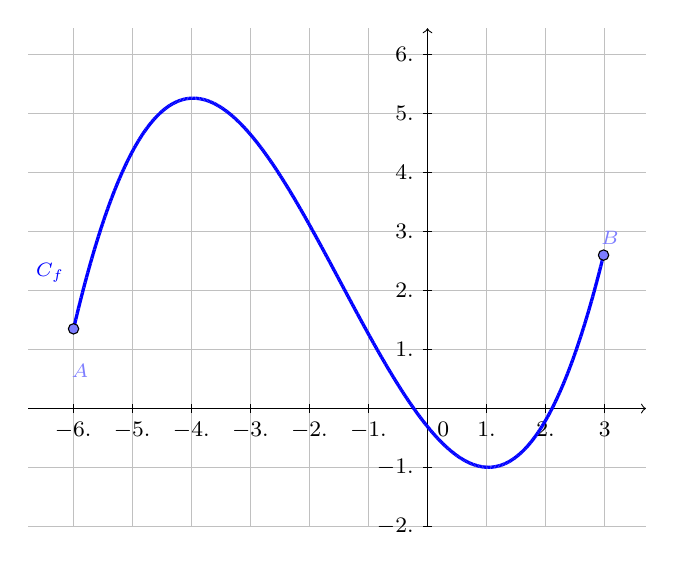
\begin{tikzpicture}[scale=0.75][line cap=round,line join=round,>=triangle 45,x=1.0cm,y=1.0cm]
\draw [color=cqcqcq,, xstep=1.0cm,ystep=1.0cm] (-6.761127226963359,-2.0022979135512675) grid (3.7,6.439987962795862);
\draw[->,color=black] (-6.761127226963359,0.) -- (3.7,0.);
\foreach \x in {-6.,-5.,-4.,-3.,-2.,-1.,1.,2.,3}
\draw[shift={(\x,0)},color=black] (0pt,2pt) -- (0pt,-2pt) node[below] {\footnotesize $\x$};
\draw[->,color=black] (0.,-2.0022979135512675) -- (0.,6.439987962795862);
\foreach \y in {-2.,-1.,1.,2.,3.,4.,5.,6.}
\draw[shift={(0,\y)},color=black] (2pt,0pt) -- (-2pt,0pt) node[left] {\footnotesize $\y$};
\draw[color=black] (0pt,-10pt) node[right] {\footnotesize $0$};
\clip(-6.761127226963359,-2.0022979135512675) rectangle (3.7,6.439987962795862);
\draw[line width=1.2pt,color=qqqqff] (-5.999999849623604,1.3225064510752396) -- (-5.999999849623604,1.3225064510752396);
\draw[line width=1.2pt,color=qqqqff] (-5.999999849623604,1.3225064510752396) -- (-5.977499850362143,1.4182293051884463);
\draw[line width=1.2pt,color=qqqqff] (-5.977499850362143,1.4182293051884463) -- (-5.954999851100682,1.5125826023245161);
\draw[line width=1.2pt,color=qqqqff] (-5.954999851100682,1.5125826023245161) -- (-5.932499851839221,1.6055731768577695);
\draw[line width=1.2pt,color=qqqqff] (-5.932499851839221,1.6055731768577695) -- (-5.90999985257776,1.6972078631625411);
\draw[line width=1.2pt,color=qqqqff] (-5.90999985257776,1.6972078631625411) -- (-5.887499853316299,1.7874934956131558);
\draw[line width=1.2pt,color=qqqqff] (-5.887499853316299,1.7874934956131558) -- (-5.8649998540548385,1.8764369085839396);
\draw[line width=1.2pt,color=qqqqff] (-5.8649998540548385,1.8764369085839396) -- (-5.8424998547933775,1.9640449364492132);
\draw[line width=1.2pt,color=qqqqff] (-5.8424998547933775,1.9640449364492132) -- (-5.819999855531917,2.0503244135833176);
\draw[line width=1.2pt,color=qqqqff] (-5.819999855531917,2.0503244135833176) -- (-5.797499856270456,2.135282174360568);
\draw[line width=1.2pt,color=qqqqff] (-5.797499856270456,2.135282174360568) -- (-5.774999857008995,2.218925053155296);
\draw[line width=1.2pt,color=qqqqff] (-5.774999857008995,2.218925053155296) -- (-5.752499857747534,2.301259884341827);
\draw[line width=1.2pt,color=qqqqff] (-5.752499857747534,2.301259884341827) -- (-5.729999858486073,2.382293502294491);
\draw[line width=1.2pt,color=qqqqff] (-5.729999858486073,2.382293502294491) -- (-5.707499859224612,2.4620327413876133);
\draw[line width=1.2pt,color=qqqqff] (-5.707499859224612,2.4620327413876133) -- (-5.684999859963151,2.54048443599552);
\draw[line width=1.2pt,color=qqqqff] (-5.684999859963151,2.54048443599552) -- (-5.66249986070169,2.61765542049254);
\draw[line width=1.2pt,color=qqqqff] (-5.66249986070169,2.61765542049254) -- (-5.639999861440229,2.693552529252998);
\draw[line width=1.2pt,color=qqqqff] (-5.639999861440229,2.693552529252998) -- (-5.617499862178768,2.76818259665122);
\draw[line width=1.2pt,color=qqqqff] (-5.617499862178768,2.76818259665122) -- (-5.594999862917307,2.841552457061538);
\draw[line width=1.2pt,color=qqqqff] (-5.594999862917307,2.841552457061538) -- (-5.572499863655846,2.9136689448582764);
\draw[line width=1.2pt,color=qqqqff] (-5.572499863655846,2.9136689448582764) -- (-5.549999864394385,2.984538894415761);
\draw[line width=1.2pt,color=qqqqff] (-5.549999864394385,2.984538894415761) -- (-5.527499865132924,3.0541691401083217);
\draw[line width=1.2pt,color=qqqqff] (-5.527499865132924,3.0541691401083217) -- (-5.504999865871463,3.1225665163102825);
\draw[line width=1.2pt,color=qqqqff] (-5.504999865871463,3.1225665163102825) -- (-5.482499866610002,3.189737857395969);
\draw[line width=1.2pt,color=qqqqff] (-5.482499866610002,3.189737857395969) -- (-5.459999867348541,3.2556899977397142);
\draw[line width=1.2pt,color=qqqqff] (-5.459999867348541,3.2556899977397142) -- (-5.43749986808708,3.320429771715839);
\draw[line width=1.2pt,color=qqqqff] (-5.43749986808708,3.320429771715839) -- (-5.414999868825619,3.3839640136986753);
\draw[line width=1.2pt,color=qqqqff] (-5.414999868825619,3.3839640136986753) -- (-5.392499869564158,3.446299558062544);
\draw[line width=1.2pt,color=qqqqff] (-5.392499869564158,3.446299558062544) -- (-5.369999870302697,3.50744323918178);
\draw[line width=1.2pt,color=qqqqff] (-5.369999870302697,3.50744323918178) -- (-5.3474998710412365,3.5674018914307046);
\draw[line width=1.2pt,color=qqqqff] (-5.3474998710412365,3.5674018914307046) -- (-5.3249998717797755,3.6261823491836473);
\draw[line width=1.2pt,color=qqqqff] (-5.3249998717797755,3.6261823491836473) -- (-5.302499872518315,3.683791446814934);
\draw[line width=1.2pt,color=qqqqff] (-5.302499872518315,3.683791446814934) -- (-5.279999873256854,3.740236018698892);
\draw[line width=1.2pt,color=qqqqff] (-5.279999873256854,3.740236018698892) -- (-5.257499873995393,3.795522899209843);
\draw[line width=1.2pt,color=qqqqff] (-5.257499873995393,3.795522899209843) -- (-5.234999874733932,3.8496589227221274);
\draw[line width=1.2pt,color=qqqqff] (-5.234999874733932,3.8496589227221274) -- (-5.212499875472471,3.9026509236100613);
\draw[line width=1.2pt,color=qqqqff] (-5.212499875472471,3.9026509236100613) -- (-5.18999987621101,3.9545057362479734);
\draw[line width=1.2pt,color=qqqqff] (-5.18999987621101,3.9545057362479734) -- (-5.167499876949549,4.00523019501019);
\draw[line width=1.2pt,color=qqqqff] (-5.167499876949549,4.00523019501019) -- (-5.144999877688088,4.054831134271043);
\draw[line width=1.2pt,color=qqqqff] (-5.144999877688088,4.054831134271043) -- (-5.122499878426627,4.103315388404855);
\draw[line width=1.2pt,color=qqqqff] (-5.122499878426627,4.103315388404855) -- (-5.099999879165166,4.150689791785956);
\draw[line width=1.2pt,color=qqqqff] (-5.099999879165166,4.150689791785956) -- (-5.077499879903705,4.196961178788672);
\draw[line width=1.2pt,color=qqqqff] (-5.077499879903705,4.196961178788672) -- (-5.054999880642244,4.242136383787326);
\draw[line width=1.2pt,color=qqqqff] (-5.054999880642244,4.242136383787326) -- (-5.032499881380783,4.286222241156248);
\draw[line width=1.2pt,color=qqqqff] (-5.032499881380783,4.286222241156248) -- (-5.009999882119322,4.329225585269769);
\draw[line width=1.2pt,color=qqqqff] (-5.009999882119322,4.329225585269769) -- (-4.987499882857861,4.371153250502211);
\draw[line width=1.2pt,color=qqqqff] (-4.987499882857861,4.371153250502211) -- (-4.9649998835964,4.4120120712279);
\draw[line width=1.2pt,color=qqqqff] (-4.9649998835964,4.4120120712279) -- (-4.942499884334939,4.451808881821168);
\draw[line width=1.2pt,color=qqqqff] (-4.942499884334939,4.451808881821168) -- (-4.919999885073478,4.490550516656337);
\draw[line width=1.2pt,color=qqqqff] (-4.919999885073478,4.490550516656337) -- (-4.897499885812017,4.528243810107739);
\draw[line width=1.2pt,color=qqqqff] (-4.897499885812017,4.528243810107739) -- (-4.874999886550556,4.564895596549698);
\draw[line width=1.2pt,color=qqqqff] (-4.874999886550556,4.564895596549698) -- (-4.852499887289095,4.60051271035654);
\draw[line width=1.2pt,color=qqqqff] (-4.852499887289095,4.60051271035654) -- (-4.8299998880276345,4.635101985902594);
\draw[line width=1.2pt,color=qqqqff] (-4.8299998880276345,4.635101985902594) -- (-4.8074998887661735,4.668670257562186);
\draw[line width=1.2pt,color=qqqqff] (-4.8074998887661735,4.668670257562186) -- (-4.7849998895047126,4.701224359709642);
\draw[line width=1.2pt,color=qqqqff] (-4.7849998895047126,4.701224359709642) -- (-4.762499890243252,4.7327711267192925);
\draw[line width=1.2pt,color=qqqqff] (-4.762499890243252,4.7327711267192925) -- (-4.739999890981791,4.763317392965464);
\draw[line width=1.2pt,color=qqqqff] (-4.739999890981791,4.763317392965464) -- (-4.71749989172033,4.79286999282248);
\draw[line width=1.2pt,color=qqqqff] (-4.71749989172033,4.79286999282248) -- (-4.694999892458869,4.82143576066467);
\draw[line width=1.2pt,color=qqqqff] (-4.694999892458869,4.82143576066467) -- (-4.672499893197408,4.849021530866358);
\draw[line width=1.2pt,color=qqqqff] (-4.672499893197408,4.849021530866358) -- (-4.649999893935947,4.8756341378018755);
\draw[line width=1.2pt,color=qqqqff] (-4.649999893935947,4.8756341378018755) -- (-4.627499894674486,4.901280415845546);
\draw[line width=1.2pt,color=qqqqff] (-4.627499894674486,4.901280415845546) -- (-4.604999895413025,4.925967199371699);
\draw[line width=1.2pt,color=qqqqff] (-4.604999895413025,4.925967199371699) -- (-4.582499896151564,4.949701322754661);
\draw[line width=1.2pt,color=qqqqff] (-4.582499896151564,4.949701322754661) -- (-4.559999896890103,4.972489620368759);
\draw[line width=1.2pt,color=qqqqff] (-4.559999896890103,4.972489620368759) -- (-4.537499897628642,4.994338926588318);
\draw[line width=1.2pt,color=qqqqff] (-4.537499897628642,4.994338926588318) -- (-4.514999898367181,5.015256075787666);
\draw[line width=1.2pt,color=qqqqff] (-4.514999898367181,5.015256075787666) -- (-4.49249989910572,5.035247902341131);
\draw[line width=1.2pt,color=qqqqff] (-4.49249989910572,5.035247902341131) -- (-4.469999899844259,5.0543212406230404);
\draw[line width=1.2pt,color=qqqqff] (-4.469999899844259,5.0543212406230404) -- (-4.447499900582798,5.072482925007719);
\draw[line width=1.2pt,color=qqqqff] (-4.447499900582798,5.072482925007719) -- (-4.424999901321337,5.089739789869498);
\draw[line width=1.2pt,color=qqqqff] (-4.424999901321337,5.089739789869498) -- (-4.402499902059876,5.106098669582698);
\draw[line width=1.2pt,color=qqqqff] (-4.402499902059876,5.106098669582698) -- (-4.379999902798415,5.121566398521651);
\draw[line width=1.2pt,color=qqqqff] (-4.379999902798415,5.121566398521651) -- (-4.357499903536954,5.136149811060681);
\draw[line width=1.2pt,color=qqqqff] (-4.357499903536954,5.136149811060681) -- (-4.334999904275493,5.149855741574119);
\draw[line width=1.2pt,color=qqqqff] (-4.334999904275493,5.149855741574119) -- (-4.3124999050140325,5.162691024436287);
\draw[line width=1.2pt,color=qqqqff] (-4.3124999050140325,5.162691024436287) -- (-4.2899999057525715,5.174662494021517);
\draw[line width=1.2pt,color=qqqqff] (-4.2899999057525715,5.174662494021517) -- (-4.2674999064911106,5.185776984704131);
\draw[line width=1.2pt,color=qqqqff] (-4.2674999064911106,5.185776984704131) -- (-4.24499990722965,5.196041330858462);
\draw[line width=1.2pt,color=qqqqff] (-4.24499990722965,5.196041330858462) -- (-4.222499907968189,5.205462366858829);
\draw[line width=1.2pt,color=qqqqff] (-4.222499907968189,5.205462366858829) -- (-4.199999908706728,5.2140469270795675);
\draw[line width=1.2pt,color=qqqqff] (-4.199999908706728,5.2140469270795675) -- (-4.177499909445267,5.2218018458949995);
\draw[line width=1.2pt,color=qqqqff] (-4.177499909445267,5.2218018458949995) -- (-4.154999910183806,5.228733957679453);
\draw[line width=1.2pt,color=qqqqff] (-4.154999910183806,5.228733957679453) -- (-4.132499910922345,5.234850096807254);
\draw[line width=1.2pt,color=qqqqff] (-4.132499910922345,5.234850096807254) -- (-4.109999911660884,5.240157097652734);
\draw[line width=1.2pt,color=qqqqff] (-4.109999911660884,5.240157097652734) -- (-4.087499912399423,5.244661794590212);
\draw[line width=1.2pt,color=qqqqff] (-4.087499912399423,5.244661794590212) -- (-4.064999913137962,5.248371021994022);
\draw[line width=1.2pt,color=qqqqff] (-4.064999913137962,5.248371021994022) -- (-4.042499913876501,5.251291614238488);
\draw[line width=1.2pt,color=qqqqff] (-4.042499913876501,5.251291614238488) -- (-4.01999991461504,5.253430405697938);
\draw[line width=1.2pt,color=qqqqff] (-4.01999991461504,5.253430405697938) -- (-3.9974999153535786,5.254794230746697);
\draw[line width=1.2pt,color=qqqqff] (-3.9974999153535786,5.254794230746697) -- (-3.9749999160921172,5.255389923759097);
\draw[line width=1.2pt,color=qqqqff] (-3.9749999160921172,5.255389923759097) -- (-3.952499916830656,5.255224319109459);
\draw[line width=1.2pt,color=qqqqff] (-3.952499916830656,5.255224319109459) -- (-3.9299999175691944,5.254304251172112);
\draw[line width=1.2pt,color=qqqqff] (-3.9299999175691944,5.254304251172112) -- (-3.907499918307733,5.252636554321385);
\draw[line width=1.2pt,color=qqqqff] (-3.907499918307733,5.252636554321385) -- (-3.8849999190462716,5.250228062931603);
\draw[line width=1.2pt,color=qqqqff] (-3.8849999190462716,5.250228062931603) -- (-3.86249991978481,5.247085611377095);
\draw[line width=1.2pt,color=qqqqff] (-3.86249991978481,5.247085611377095) -- (-3.839999920523349,5.2432160340321845);
\draw[line width=1.2pt,color=qqqqff] (-3.839999920523349,5.2432160340321845) -- (-3.8174999212618874,5.238626165271203);
\draw[line width=1.2pt,color=qqqqff] (-3.8174999212618874,5.238626165271203) -- (-3.794999922000426,5.233322839468474);
\draw[line width=1.2pt,color=qqqqff] (-3.794999922000426,5.233322839468474) -- (-3.7724999227389646,5.227312890998324);
\draw[line width=1.2pt,color=qqqqff] (-3.7724999227389646,5.227312890998324) -- (-3.749999923477503,5.220603154235085);
\draw[line width=1.2pt,color=qqqqff] (-3.749999923477503,5.220603154235085) -- (-3.727499924216042,5.213200463553079);
\draw[line width=1.2pt,color=qqqqff] (-3.727499924216042,5.213200463553079) -- (-3.7049999249545804,5.205111653326633);
\draw[line width=1.2pt,color=qqqqff] (-3.7049999249545804,5.205111653326633) -- (-3.682499925693119,5.196343557930078);
\draw[line width=1.2pt,color=qqqqff] (-3.682499925693119,5.196343557930078) -- (-3.6599999264316576,5.186903011737738);
\draw[line width=1.2pt,color=qqqqff] (-3.6599999264316576,5.186903011737738) -- (-3.637499927170196,5.1767968491239404);
\draw[line width=1.2pt,color=qqqqff] (-3.637499927170196,5.1767968491239404) -- (-3.614999927908735,5.166031904463013);
\draw[line width=1.2pt,color=qqqqff] (-3.614999927908735,5.166031904463013) -- (-3.5924999286472734,5.154615012129282);
\draw[line width=1.2pt,color=qqqqff] (-3.5924999286472734,5.154615012129282) -- (-3.569999929385812,5.142553006497075);
\draw[line width=1.2pt,color=qqqqff] (-3.569999929385812,5.142553006497075) -- (-3.5474999301243506,5.129852721940719);
\draw[line width=1.2pt,color=qqqqff] (-3.5474999301243506,5.129852721940719) -- (-3.524999930862889,5.1165209928345385);
\draw[line width=1.2pt,color=qqqqff] (-3.524999930862889,5.1165209928345385) -- (-3.502499931601428,5.102564653552865);
\draw[line width=1.2pt,color=qqqqff] (-3.502499931601428,5.102564653552865) -- (-3.4799999323399664,5.087990538470023);
\draw[line width=1.2pt,color=qqqqff] (-3.4799999323399664,5.087990538470023) -- (-3.457499933078505,5.072805481960338);
\draw[line width=1.2pt,color=qqqqff] (-3.457499933078505,5.072805481960338) -- (-3.4349999338170436,5.057016318398142);
\draw[line width=1.2pt,color=qqqqff] (-3.4349999338170436,5.057016318398142) -- (-3.412499934555582,5.040629882157757);
\draw[line width=1.2pt,color=qqqqff] (-3.412499934555582,5.040629882157757) -- (-3.389999935294121,5.023653007613511);
\draw[line width=1.2pt,color=qqqqff] (-3.389999935294121,5.023653007613511) -- (-3.3674999360326594,5.006092529139733);
\draw[line width=1.2pt,color=qqqqff] (-3.3674999360326594,5.006092529139733) -- (-3.344999936771198,4.9879552811107475);
\draw[line width=1.2pt,color=qqqqff] (-3.344999936771198,4.9879552811107475) -- (-3.3224999375097366,4.969248097900883);
\draw[line width=1.2pt,color=qqqqff] (-3.3224999375097366,4.969248097900883) -- (-3.299999938248275,4.949977813884467);
\draw[line width=1.2pt,color=qqqqff] (-3.299999938248275,4.949977813884467) -- (-3.277499938986814,4.9301512634358255);
\draw[line width=1.2pt,color=qqqqff] (-3.277499938986814,4.9301512634358255) -- (-3.2549999397253524,4.909775280929287);
\draw[line width=1.2pt,color=qqqqff] (-3.2549999397253524,4.909775280929287) -- (-3.232499940463891,4.8888567007391766);
\draw[line width=1.2pt,color=qqqqff] (-3.232499940463891,4.8888567007391766) -- (-3.2099999412024296,4.867402357239821);
\draw[line width=1.2pt,color=qqqqff] (-3.2099999412024296,4.867402357239821) -- (-3.187499941940968,4.84541908480555);
\draw[line width=1.2pt,color=qqqqff] (-3.187499941940968,4.84541908480555) -- (-3.164999942679507,4.822913717810686);
\draw[line width=1.2pt,color=qqqqff] (-3.164999942679507,4.822913717810686) -- (-3.1424999434180454,4.799893090629561);
\draw[line width=1.2pt,color=qqqqff] (-3.1424999434180454,4.799893090629561) -- (-3.119999944156584,4.776364037636498);
\draw[line width=1.2pt,color=qqqqff] (-3.119999944156584,4.776364037636498) -- (-3.0974999448951226,4.752333393205828);
\draw[line width=1.2pt,color=qqqqff] (-3.0974999448951226,4.752333393205828) -- (-3.074999945633661,4.727807991711876);
\draw[line width=1.2pt,color=qqqqff] (-3.074999945633661,4.727807991711876) -- (-3.0524999463722,4.702794667528967);
\draw[line width=1.2pt,color=qqqqff] (-3.0524999463722,4.702794667528967) -- (-3.0299999471107384,4.677300255031431);
\draw[line width=1.2pt,color=qqqqff] (-3.0299999471107384,4.677300255031431) -- (-3.007499947849277,4.651331588593593);
\draw[line width=1.2pt,color=qqqqff] (-3.007499947849277,4.651331588593593) -- (-2.9849999485878156,4.624895502589783);
\draw[line width=1.2pt,color=qqqqff] (-2.9849999485878156,4.624895502589783) -- (-2.962499949326354,4.597998831394324);
\draw[line width=1.2pt,color=qqqqff] (-2.962499949326354,4.597998831394324) -- (-2.939999950064893,4.570648409381545);
\draw[line width=1.2pt,color=qqqqff] (-2.939999950064893,4.570648409381545) -- (-2.9174999508034314,4.5428510709257734);
\draw[line width=1.2pt,color=qqqqff] (-2.9174999508034314,4.5428510709257734) -- (-2.89499995154197,4.514613650401336);
\draw[line width=1.2pt,color=qqqqff] (-2.89499995154197,4.514613650401336) -- (-2.8724999522805086,4.48594298218256);
\draw[line width=1.2pt,color=qqqqff] (-2.8724999522805086,4.48594298218256) -- (-2.849999953019047,4.45684590064377);
\draw[line width=1.2pt,color=qqqqff] (-2.849999953019047,4.45684590064377) -- (-2.827499953757586,4.427329240159295);
\draw[line width=1.2pt,color=qqqqff] (-2.827499953757586,4.427329240159295) -- (-2.8049999544961244,4.397399835103464);
\draw[line width=1.2pt,color=qqqqff] (-2.8049999544961244,4.397399835103464) -- (-2.782499955234663,4.367064519850601);
\draw[line width=1.2pt,color=qqqqff] (-2.782499955234663,4.367064519850601) -- (-2.7599999559732016,4.336330128775033);
\draw[line width=1.2pt,color=qqqqff] (-2.7599999559732016,4.336330128775033) -- (-2.73749995671174,4.305203496251089);
\draw[line width=1.2pt,color=qqqqff] (-2.73749995671174,4.305203496251089) -- (-2.714999957450279,4.273691456653095);
\draw[line width=1.2pt,color=qqqqff] (-2.714999957450279,4.273691456653095) -- (-2.6924999581888174,4.241800844355377);
\draw[line width=1.2pt,color=qqqqff] (-2.6924999581888174,4.241800844355377) -- (-2.669999958927356,4.209538493732264);
\draw[line width=1.2pt,color=qqqqff] (-2.669999958927356,4.209538493732264) -- (-2.6474999596658946,4.176911239158082);
\draw[line width=1.2pt,color=qqqqff] (-2.6474999596658946,4.176911239158082) -- (-2.624999960404433,4.1439259150071575);
\draw[line width=1.2pt,color=qqqqff] (-2.624999960404433,4.1439259150071575) -- (-2.6024999611429718,4.1105893556538184);
\draw[line width=1.2pt,color=qqqqff] (-2.6024999611429718,4.1105893556538184) -- (-2.5799999618815104,4.07690839547239);
\draw[line width=1.2pt,color=qqqqff] (-2.5799999618815104,4.07690839547239) -- (-2.557499962620049,4.042889868837203);
\draw[line width=1.2pt,color=qqqqff] (-2.557499962620049,4.042889868837203) -- (-2.5349999633585876,4.00854061012258);
\draw[line width=1.2pt,color=qqqqff] (-2.5349999633585876,4.00854061012258) -- (-2.512499964097126,3.973867453702851);
\draw[line width=1.2pt,color=qqqqff] (-2.512499964097126,3.973867453702851) -- (-2.4899999648356648,3.9388772339523404);
\draw[line width=1.2pt,color=qqqqff] (-2.4899999648356648,3.9388772339523404) -- (-2.4674999655742034,3.9035767852453787);
\draw[line width=1.2pt,color=qqqqff] (-2.4674999655742034,3.9035767852453787) -- (-2.444999966312742,3.867972941956291);
\draw[line width=1.2pt,color=qqqqff] (-2.444999966312742,3.867972941956291) -- (-2.4224999670512806,3.832072538459403);
\draw[line width=1.2pt,color=qqqqff] (-2.4224999670512806,3.832072538459403) -- (-2.399999967789819,3.7958824091290446);
\draw[line width=1.2pt,color=qqqqff] (-2.399999967789819,3.7958824091290446) -- (-2.3774999685283578,3.759409388339541);
\draw[line width=1.2pt,color=qqqqff] (-2.3774999685283578,3.759409388339541) -- (-2.3549999692668964,3.7226603104652187);
\draw[line width=1.2pt,color=qqqqff] (-2.3549999692668964,3.7226603104652187) -- (-2.332499970005435,3.685642009880406);
\draw[line width=1.2pt,color=qqqqff] (-2.332499970005435,3.685642009880406) -- (-2.3099999707439736,3.6483613209594288);
\draw[line width=1.2pt,color=qqqqff] (-2.3099999707439736,3.6483613209594288) -- (-2.287499971482512,3.6108250780766147);
\draw[line width=1.2pt,color=qqqqff] (-2.287499971482512,3.6108250780766147) -- (-2.2649999722210508,3.573040115606292);
\draw[line width=1.2pt,color=qqqqff] (-2.2649999722210508,3.573040115606292) -- (-2.2424999729595894,3.5350132679227855);
\draw[line width=1.2pt,color=qqqqff] (-2.2424999729595894,3.5350132679227855) -- (-2.219999973698128,3.4967513694004224);
\draw[line width=1.2pt,color=qqqqff] (-2.219999973698128,3.4967513694004224) -- (-2.1974999744366666,3.4582612544135314);
\draw[line width=1.2pt,color=qqqqff] (-2.1974999744366666,3.4582612544135314) -- (-2.174999975175205,3.4195497573364384);
\draw[line width=1.2pt,color=qqqqff] (-2.174999975175205,3.4195497573364384) -- (-2.1524999759137438,3.3806237125434713);
\draw[line width=1.2pt,color=qqqqff] (-2.1524999759137438,3.3806237125434713) -- (-2.1299999766522824,3.3414899544089542);
\draw[line width=1.2pt,color=qqqqff] (-2.1299999766522824,3.3414899544089542) -- (-2.107499977390821,3.3021553173072182);
\draw[line width=1.2pt,color=qqqqff] (-2.107499977390821,3.3021553173072182) -- (-2.0849999781293596,3.2626266356125875);
\draw[line width=1.2pt,color=qqqqff] (-2.0849999781293596,3.2626266356125875) -- (-2.062499978867898,3.2229107436993907);
\draw[line width=1.2pt,color=qqqqff] (-2.062499978867898,3.2229107436993907) -- (-2.0399999796064368,3.183014475941953);
\draw[line width=1.2pt,color=qqqqff] (-2.0399999796064368,3.183014475941953) -- (-2.0174999803449754,3.142944666714603);
\draw[line width=1.2pt,color=qqqqff] (-2.0174999803449754,3.142944666714603) -- (-1.994999981083514,3.1027081503916674);
\draw[line width=1.2pt,color=qqqqff] (-1.994999981083514,3.1027081503916674) -- (-1.9724999818220526,3.0623117613474724);
\draw[line width=1.2pt,color=qqqqff] (-1.9724999818220526,3.0623117613474724) -- (-1.9499999825605911,3.021762333956346);
\draw[line width=1.2pt,color=qqqqff] (-1.9499999825605911,3.021762333956346) -- (-1.9274999832991297,2.981066702592615);
\draw[line width=1.2pt,color=qqqqff] (-1.9274999832991297,2.981066702592615) -- (-1.9049999840376683,2.9402317016306063);
\draw[line width=1.2pt,color=qqqqff] (-1.9049999840376683,2.9402317016306063) -- (-1.882499984776207,2.8992641654446465);
\draw[line width=1.2pt,color=qqqqff] (-1.882499984776207,2.8992641654446465) -- (-1.8599999855147455,2.858170928409062);
\draw[line width=1.2pt,color=qqqqff] (-1.8599999855147455,2.858170928409062) -- (-1.8374999862532841,2.816958824898182);
\draw[line width=1.2pt,color=qqqqff] (-1.8374999862532841,2.816958824898182) -- (-1.8149999869918227,2.7756346892863317);
\draw[line width=1.2pt,color=qqqqff] (-1.8149999869918227,2.7756346892863317) -- (-1.7924999877303613,2.734205355947839);
\draw[line width=1.2pt,color=qqqqff] (-1.7924999877303613,2.734205355947839) -- (-1.7699999884689,2.69267765925703);
\draw[line width=1.2pt,color=qqqqff] (-1.7699999884689,2.69267765925703) -- (-1.7474999892074385,2.651058433588233);
\draw[line width=1.2pt,color=qqqqff] (-1.7474999892074385,2.651058433588233) -- (-1.7249999899459771,2.609354513315774);
\draw[line width=1.2pt,color=qqqqff] (-1.7249999899459771,2.609354513315774) -- (-1.7024999906845157,2.56757273281398);
\draw[line width=1.2pt,color=qqqqff] (-1.7024999906845157,2.56757273281398) -- (-1.6799999914230543,2.525719926457178);
\draw[line width=1.2pt,color=qqqqff] (-1.6799999914230543,2.525719926457178) -- (-1.657499992161593,2.483802928619696);
\draw[line width=1.2pt,color=qqqqff] (-1.657499992161593,2.483802928619696) -- (-1.6349999929001315,2.4418285736758603);
\draw[line width=1.2pt,color=qqqqff] (-1.6349999929001315,2.4418285736758603) -- (-1.6124999936386701,2.399803695999997);
\draw[line width=1.2pt,color=qqqqff] (-1.6124999936386701,2.399803695999997) -- (-1.5899999943772087,2.3577351299664344);
\draw[line width=1.2pt,color=qqqqff] (-1.5899999943772087,2.3577351299664344) -- (-1.5674999951157473,2.3156297099495);
\draw[line width=1.2pt,color=qqqqff] (-1.5674999951157473,2.3156297099495) -- (-1.544999995854286,2.273494270323519);
\draw[line width=1.2pt,color=qqqqff] (-1.544999995854286,2.273494270323519) -- (-1.5224999965928245,2.2313356454628193);
\draw[line width=1.2pt,color=qqqqff] (-1.5224999965928245,2.2313356454628193) -- (-1.4999999973313631,2.189160669741728);
\draw[line width=1.2pt,color=qqqqff] (-1.4999999973313631,2.189160669741728) -- (-1.4774999980699017,2.1469761775345724);
\draw[line width=1.2pt,color=qqqqff] (-1.4774999980699017,2.1469761775345724) -- (-1.4549999988084403,2.104789003215679);
\draw[line width=1.2pt,color=qqqqff] (-1.4549999988084403,2.104789003215679) -- (-1.432499999546979,2.0626059811593747);
\draw[line width=1.2pt,color=qqqqff] (-1.432499999546979,2.0626059811593747) -- (-1.4100000002855175,2.0204339457399865);
\draw[line width=1.2pt,color=qqqqff] (-1.4100000002855175,2.0204339457399865) -- (-1.3875000010240561,1.9782797313318423);
\draw[line width=1.2pt,color=qqqqff] (-1.3875000010240561,1.9782797313318423) -- (-1.3650000017625947,1.9361501723092687);
\draw[line width=1.2pt,color=qqqqff] (-1.3650000017625947,1.9361501723092687) -- (-1.3425000025011333,1.894052103046592);
\draw[line width=1.2pt,color=qqqqff] (-1.3425000025011333,1.894052103046592) -- (-1.320000003239672,1.8519923579181392);
\draw[line width=1.2pt,color=qqqqff] (-1.320000003239672,1.8519923579181392) -- (-1.2975000039782105,1.8099777712982386);
\draw[line width=1.2pt,color=qqqqff] (-1.2975000039782105,1.8099777712982386) -- (-1.2750000047167491,1.768015177561216);
\draw[line width=1.2pt,color=qqqqff] (-1.2750000047167491,1.768015177561216) -- (-1.2525000054552877,1.726111411081399);
\draw[line width=1.2pt,color=qqqqff] (-1.2525000054552877,1.726111411081399) -- (-1.2300000061938263,1.6842733062331146);
\draw[line width=1.2pt,color=qqqqff] (-1.2300000061938263,1.6842733062331146) -- (-1.207500006932365,1.6425076973906894);
\draw[line width=1.2pt,color=qqqqff] (-1.207500006932365,1.6425076973906894) -- (-1.1850000076709035,1.6008214189284504);
\draw[line width=1.2pt,color=qqqqff] (-1.1850000076709035,1.6008214189284504) -- (-1.1625000084094421,1.5592213052207247);
\draw[line width=1.2pt,color=qqqqff] (-1.1625000084094421,1.5592213052207247) -- (-1.1400000091479807,1.5177141906418403);
\draw[line width=1.2pt,color=qqqqff] (-1.1400000091479807,1.5177141906418403) -- (-1.1175000098865193,1.4763069095661225);
\draw[line width=1.2pt,color=qqqqff] (-1.1175000098865193,1.4763069095661225) -- (-1.095000010625058,1.4350062963678991);
\draw[line width=1.2pt,color=qqqqff] (-1.095000010625058,1.4350062963678991) -- (-1.0725000113635965,1.3938191854214979);
\draw[line width=1.2pt,color=qqqqff] (-1.0725000113635965,1.3938191854214979) -- (-1.0500000121021351,1.3527524111012448);
\draw[line width=1.2pt,color=qqqqff] (-1.0500000121021351,1.3527524111012448) -- (-1.0275000128406737,1.3118128077814668);
\draw[line width=1.2pt,color=qqqqff] (-1.0275000128406737,1.3118128077814668) -- (-1.0050000135792123,1.2710072098364917);
\draw[line width=1.2pt,color=qqqqff] (-1.0050000135792123,1.2710072098364917) -- (-0.982500014317751,1.230342451640646);
\draw[line width=1.2pt,color=qqqqff] (-0.982500014317751,1.230342451640646) -- (-0.9600000150562897,1.189825367568257);
\draw[line width=1.2pt,color=qqqqff] (-0.9600000150562897,1.189825367568257) -- (-0.9375000157948284,1.1494627919936513);
\draw[line width=1.2pt,color=qqqqff] (-0.9375000157948284,1.1494627919936513) -- (-0.9150000165333672,1.109261559291156);
\draw[line width=1.2pt,color=qqqqff] (-0.9150000165333672,1.109261559291156) -- (-0.8925000172719059,1.0692285038350988);
\draw[line width=1.2pt,color=qqqqff] (-0.8925000172719059,1.0692285038350988) -- (-0.8700000180104446,1.029370459999806);
\draw[line width=1.2pt,color=qqqqff] (-0.8700000180104446,1.029370459999806) -- (-0.8475000187489833,0.9896942621596042);
\draw[line width=1.2pt,color=qqqqff] (-0.8475000187489833,0.9896942621596042) -- (-0.825000019487522,0.9502067446888213);
\draw[line width=1.2pt,color=qqqqff] (-0.825000019487522,0.9502067446888213) -- (-0.8025000202260607,0.9109147419617839);
\draw[line width=1.2pt,color=qqqqff] (-0.8025000202260607,0.9109147419617839) -- (-0.7800000209645994,0.8718250883528192);
\draw[line width=1.2pt,color=qqqqff] (-0.7800000209645994,0.8718250883528192) -- (-0.7575000217031381,0.8329446182362538);
\draw[line width=1.2pt,color=qqqqff] (-0.7575000217031381,0.8329446182362538) -- (-0.7350000224416768,0.7942801659864148);
\draw[line width=1.2pt,color=qqqqff] (-0.7350000224416768,0.7942801659864148) -- (-0.7125000231802155,0.7558385659776296);
\draw[line width=1.2pt,color=qqqqff] (-0.7125000231802155,0.7558385659776296) -- (-0.6900000239187543,0.7176266525842251);
\draw[line width=1.2pt,color=qqqqff] (-0.6900000239187543,0.7176266525842251) -- (-0.667500024657293,0.6796512601805279);
\draw[line width=1.2pt,color=qqqqff] (-0.667500024657293,0.6796512601805279) -- (-0.6450000253958317,0.6419192231408654);
\draw[line width=1.2pt,color=qqqqff] (-0.6450000253958317,0.6419192231408654) -- (-0.6225000261343704,0.6044373758395644);
\draw[line width=1.2pt,color=qqqqff] (-0.6225000261343704,0.6044373758395644) -- (-0.6000000268729091,0.567212552650952);
\draw[line width=1.2pt,color=qqqqff] (-0.6000000268729091,0.567212552650952) -- (-0.5775000276114478,0.5302515879493553);
\draw[line width=1.2pt,color=qqqqff] (-0.5775000276114478,0.5302515879493553) -- (-0.5550000283499865,0.49356131610910114);
\draw[line width=1.2pt,color=qqqqff] (-0.5550000283499865,0.49356131610910114) -- (-0.5325000290885252,0.4571485715045168);
\draw[line width=1.2pt,color=qqqqff] (-0.5325000290885252,0.4571485715045168) -- (-0.5100000298270639,0.42102018850992895);
\draw[line width=1.2pt,color=qqqqff] (-0.5100000298270639,0.42102018850992895) -- (-0.48750003056560265,0.38518300149966456);
\draw[line width=1.2pt,color=qqqqff] (-0.48750003056560265,0.38518300149966456) -- (-0.46500003130414136,0.349643844848051);
\draw[line width=1.2pt,color=qqqqff] (-0.46500003130414136,0.349643844848051) -- (-0.44250003204268007,0.3144095529294151);
\draw[line width=1.2pt,color=qqqqff] (-0.44250003204268007,0.3144095529294151) -- (-0.4200000327812188,0.2794869601180837);
\draw[line width=1.2pt,color=qqqqff] (-0.4200000327812188,0.2794869601180837) -- (-0.3975000335197575,0.24488290078838404);
\draw[line width=1.2pt,color=qqqqff] (-0.3975000335197575,0.24488290078838404) -- (-0.3750000342582962,0.21060420931464297);
\draw[line width=1.2pt,color=qqqqff] (-0.3750000342582962,0.21060420931464297) -- (-0.3525000349968349,0.17665772007118763);
\draw[line width=1.2pt,color=qqqqff] (-0.3525000349968349,0.17665772007118763) -- (-0.3300000357353736,0.14305026743234506);
\draw[line width=1.2pt,color=qqqqff] (-0.3300000357353736,0.14305026743234506) -- (-0.30750003647391233,0.109788685772442);
\draw[line width=1.2pt,color=qqqqff] (-0.30750003647391233,0.109788685772442) -- (-0.28500003721245104,0.07687980946580575);
\draw[line width=1.2pt,color=qqqqff] (-0.28500003721245104,0.07687980946580575) -- (-0.26250003795098975,0.04433047288676312);
\draw[line width=1.2pt,color=qqqqff] (-0.26250003795098975,0.04433047288676312) -- (-0.24000003868952843,0.012147510409641238);
\draw[line width=1.2pt,color=qqqqff] (-0.24000003868952843,0.012147510409641238) -- (-0.21750003942806712,-0.01966224359123303);
\draw[line width=1.2pt,color=qqqqff] (-0.21750003942806712,-0.01966224359123303) -- (-0.1950000401666058,-0.05109195474153255);
\draw[line width=1.2pt,color=qqqqff] (-0.1950000401666058,-0.05109195474153255) -- (-0.17250004090514448,-0.08213478866693036);
\draw[line width=1.2pt,color=qqqqff] (-0.17250004090514448,-0.08213478866693036) -- (-0.15000004164368316,-0.11278391099309945);
\draw[line width=1.2pt,color=qqqqff] (-0.15000004164368316,-0.11278391099309945) -- (-0.12750004238222185,-0.14303248734571278);
\draw[line width=1.2pt,color=qqqqff] (-0.12750004238222185,-0.14303248734571278) -- (-0.10500004312076053,-0.1728736833504434);
\draw[line width=1.2pt,color=qqqqff] (-0.10500004312076053,-0.1728736833504434) -- (-0.08250004385929921,-0.20230066463296423);
\draw[line width=1.2pt,color=qqqqff] (-0.08250004385929921,-0.20230066463296423) -- (-0.06000004459783789,-0.23130659681894833);
\draw[line width=1.2pt,color=qqqqff] (-0.06000004459783789,-0.23130659681894833) -- (-0.037500045336376575,-0.25988464553406865);
\draw[line width=1.2pt,color=qqqqff] (-0.037500045336376575,-0.25988464553406865) -- (-0.015000046074915258,-0.28802797640399824);
\draw[line width=1.2pt,color=qqqqff] (-0.015000046074915258,-0.28802797640399824) -- (0.00749995318654606,-0.31572975505441003);
\draw[line width=1.2pt,color=qqqqff] (0.00749995318654606,-0.31572975505441003) -- (0.029999952448007378,-0.34298314711097705);
\draw[line width=1.2pt,color=qqqqff] (0.029999952448007378,-0.34298314711097705) -- (0.052499951709468695,-0.36978131819937227);
\draw[line width=1.2pt,color=qqqqff] (0.052499951709468695,-0.36978131819937227) -- (0.07499995097093001,-0.39611743394526866);
\draw[line width=1.2pt,color=qqqqff] (0.07499995097093001,-0.39611743394526866) -- (0.09749995023239133,-0.4219846599743393);
\draw[line width=1.2pt,color=qqqqff] (0.09749995023239133,-0.4219846599743393) -- (0.11999994949385265,-0.44737616191225715);
\draw[line width=1.2pt,color=qqqqff] (0.11999994949385265,-0.44737616191225715) -- (0.14249994875531397,-0.47228510538469515);
\draw[line width=1.2pt,color=qqqqff] (0.14249994875531397,-0.47228510538469515) -- (0.16499994801677528,-0.49670465601732633);
\draw[line width=1.2pt,color=qqqqff] (0.16499994801677528,-0.49670465601732633) -- (0.1874999472782366,-0.5206279794358237);
\draw[line width=1.2pt,color=qqqqff] (0.1874999472782366,-0.5206279794358237) -- (0.20999994653969792,-0.5440482412658603);
\draw[line width=1.2pt,color=qqqqff] (0.20999994653969792,-0.5440482412658603) -- (0.23249994580115924,-0.5669586071331089);
\draw[line width=1.2pt,color=qqqqff] (0.23249994580115924,-0.5669586071331089) -- (0.2549999450626206,-0.5893522426632427);
\draw[line width=1.2pt,color=qqqqff] (0.2549999450626206,-0.5893522426632427) -- (0.27749994432408187,-0.6112223134819347);
\draw[line width=1.2pt,color=qqqqff] (0.27749994432408187,-0.6112223134819347) -- (0.29999994358554316,-0.6325619852148578);
\draw[line width=1.2pt,color=qqqqff] (0.29999994358554316,-0.6325619852148578) -- (0.32249994284700445,-0.653364423487685);
\draw[line width=1.2pt,color=qqqqff] (0.32249994284700445,-0.653364423487685) -- (0.34499994210846574,-0.6736227939260894);
\draw[line width=1.2pt,color=qqqqff] (0.34499994210846574,-0.6736227939260894) -- (0.36749994136992703,-0.6933302621557439);
\draw[line width=1.2pt,color=qqqqff] (0.36749994136992703,-0.6933302621557439) -- (0.3899999406313883,-0.7124799938023215);
\draw[line width=1.2pt,color=qqqqff] (0.3899999406313883,-0.7124799938023215) -- (0.4124999398928496,-0.7310651544914951);
\draw[line width=1.2pt,color=qqqqff] (0.4124999398928496,-0.7310651544914951) -- (0.4349999391543109,-0.7490789098489379);
\draw[line width=1.2pt,color=qqqqff] (0.4349999391543109,-0.7490789098489379) -- (0.4574999384157722,-0.7665144255003228);
\draw[line width=1.2pt,color=qqqqff] (0.4574999384157722,-0.7665144255003228) -- (0.4799999376772335,-0.7833648670713228);
\draw[line width=1.2pt,color=qqqqff] (0.4799999376772335,-0.7833648670713228) -- (0.5024999369386948,-0.7996234001876108);
\draw[line width=1.2pt,color=qqqqff] (0.5024999369386948,-0.7996234001876108) -- (0.5249999362001561,-0.8152831904748599);
\draw[line width=1.2pt,color=qqqqff] (0.5249999362001561,-0.8152831904748599) -- (0.5474999354616173,-0.8303374035587432);
\draw[line width=1.2pt,color=qqqqff] (0.5474999354616173,-0.8303374035587432) -- (0.5699999347230786,-0.8447792050649334);
\draw[line width=1.2pt,color=qqqqff] (0.5699999347230786,-0.8447792050649334) -- (0.5924999339845399,-0.8586017606191036);
\draw[line width=1.2pt,color=qqqqff] (0.5924999339845399,-0.8586017606191036) -- (0.6149999332460012,-0.8717982358469271);
\draw[line width=1.2pt,color=qqqqff] (0.6149999332460012,-0.8717982358469271) -- (0.6374999325074625,-0.8843617963740764);
\draw[line width=1.2pt,color=qqqqff] (0.6374999325074625,-0.8843617963740764) -- (0.6599999317689238,-0.8962856078262249);
\draw[line width=1.2pt,color=qqqqff] (0.6599999317689238,-0.8962856078262249) -- (0.6824999310303851,-0.9075628358290453);
\draw[line width=1.2pt,color=qqqqff] (0.6824999310303851,-0.9075628358290453) -- (0.7049999302918464,-0.9181866460082108);
\draw[line width=1.2pt,color=qqqqff] (0.7049999302918464,-0.9181866460082108) -- (0.7274999295533077,-0.9281502039893944);
\draw[line width=1.2pt,color=qqqqff] (0.7274999295533077,-0.9281502039893944) -- (0.749999928814769,-0.9374466753982689);
\draw[line width=1.2pt,color=qqqqff] (0.749999928814769,-0.9374466753982689) -- (0.7724999280762302,-0.9460692258605073);
\draw[line width=1.2pt,color=qqqqff] (0.7724999280762302,-0.9460692258605073) -- (0.7949999273376915,-0.9540110210017828);
\draw[line width=1.2pt,color=qqqqff] (0.7949999273376915,-0.9540110210017828) -- (0.8174999265991528,-0.9612652264477684);
\draw[line width=1.2pt,color=qqqqff] (0.8174999265991528,-0.9612652264477684) -- (0.8399999258606141,-0.9678250078241367);
\draw[line width=1.2pt,color=qqqqff] (0.8399999258606141,-0.9678250078241367) -- (0.8624999251220754,-0.9736835307565612);
\draw[line width=1.2pt,color=qqqqff] (0.8624999251220754,-0.9736835307565612) -- (0.8849999243835367,-0.9788339608707146);
\draw[line width=1.2pt,color=qqqqff] (0.8849999243835367,-0.9788339608707146) -- (0.907499923644998,-0.9832694637922702);
\draw[line width=1.2pt,color=qqqqff] (0.907499923644998,-0.9832694637922702) -- (0.9299999229064593,-0.9869832051469004);
\draw[line width=1.2pt,color=qqqqff] (0.9299999229064593,-0.9869832051469004) -- (0.9524999221679206,-0.9899683505602787);
\draw[line width=1.2pt,color=qqqqff] (0.9524999221679206,-0.9899683505602787) -- (0.9749999214293819,-0.9922180656580778);
\draw[line width=1.2pt,color=qqqqff] (0.9749999214293819,-0.9922180656580778) -- (0.9974999206908431,-0.9937255160659709);
\draw[line width=1.2pt,color=qqqqff] (0.9974999206908431,-0.9937255160659709) -- (1.0199999199523044,-0.9944838674096311);
\draw[line width=1.2pt,color=qqqqff] (1.0199999199523044,-0.9944838674096311) -- (1.0424999192137658,-0.994486285314731);
\draw[line width=1.2pt,color=qqqqff] (1.0424999192137658,-0.994486285314731) -- (1.0649999184752272,-0.993725935406944);
\draw[line width=1.2pt,color=qqqqff] (1.0649999184752272,-0.993725935406944) -- (1.0874999177366886,-0.9921959833119427);
\draw[line width=1.2pt,color=qqqqff] (1.0874999177366886,-0.9921959833119427) -- (1.10999991699815,-0.9898895946554005);
\draw[line width=1.2pt,color=qqqqff] (1.10999991699815,-0.9898895946554005) -- (1.1324999162596114,-0.9867999350629901);
\draw[line width=1.2pt,color=qqqqff] (1.1324999162596114,-0.9867999350629901) -- (1.1549999155210728,-0.9829201701603845);
\draw[line width=1.2pt,color=qqqqff] (1.1549999155210728,-0.9829201701603845) -- (1.1774999147825342,-0.9782434655732568);
\draw[line width=1.2pt,color=qqqqff] (1.1774999147825342,-0.9782434655732568) -- (1.1999999140439956,-0.9727629869272801);
\draw[line width=1.2pt,color=qqqqff] (1.1999999140439956,-0.9727629869272801) -- (1.222499913305457,-0.9664718998481272);
\draw[line width=1.2pt,color=qqqqff] (1.222499913305457,-0.9664718998481272) -- (1.2449999125669184,-0.9593633699614712);
\draw[line width=1.2pt,color=qqqqff] (1.2449999125669184,-0.9593633699614712) -- (1.2674999118283798,-0.9514305628929849);
\draw[line width=1.2pt,color=qqqqff] (1.2674999118283798,-0.9514305628929849) -- (1.2899999110898412,-0.9426666442683415);
\draw[line width=1.2pt,color=qqqqff] (1.2899999110898412,-0.9426666442683415) -- (1.3124999103513026,-0.9330647797132139);
\draw[line width=1.2pt,color=qqqqff] (1.3124999103513026,-0.9330647797132139) -- (1.334999909612764,-0.9226181348532754);
\draw[line width=1.2pt,color=qqqqff] (1.334999909612764,-0.9226181348532754) -- (1.3574999088742254,-0.9113198753141983);
\draw[line width=1.2pt,color=qqqqff] (1.3574999088742254,-0.9113198753141983) -- (1.3799999081356868,-0.8991631667216563);
\draw[line width=1.2pt,color=qqqqff] (1.3799999081356868,-0.8991631667216563) -- (1.4024999073971482,-0.8861411747013219);
\draw[line width=1.2pt,color=qqqqff] (1.4024999073971482,-0.8861411747013219) -- (1.4249999066586096,-0.8722470648788685);
\draw[line width=1.2pt,color=qqqqff] (1.4249999066586096,-0.8722470648788685) -- (1.447499905920071,-0.8574740028799687);
\draw[line width=1.2pt,color=qqqqff] (1.447499905920071,-0.8574740028799687) -- (1.4699999051815325,-0.8418151543302959);
\draw[line width=1.2pt,color=qqqqff] (1.4699999051815325,-0.8418151543302959) -- (1.4924999044429939,-0.8252636848555228);
\draw[line width=1.2pt,color=qqqqff] (1.4924999044429939,-0.8252636848555228) -- (1.5149999037044553,-0.8078127600813223);
\draw[line width=1.2pt,color=qqqqff] (1.5149999037044553,-0.8078127600813223) -- (1.5374999029659167,-0.7894555456333677);
\draw[line width=1.2pt,color=qqqqff] (1.5374999029659167,-0.7894555456333677) -- (1.559999902227378,-0.7701852071373319);
\draw[line width=1.2pt,color=qqqqff] (1.559999902227378,-0.7701852071373319) -- (1.5824999014888395,-0.7499949102188881);
\draw[line width=1.2pt,color=qqqqff] (1.5824999014888395,-0.7499949102188881) -- (1.6049999007503009,-0.7288778205037086);
\draw[line width=1.2pt,color=qqqqff] (1.6049999007503009,-0.7288778205037086) -- (1.6274999000117623,-0.7068271036174666);
\draw[line width=1.2pt,color=qqqqff] (1.6274999000117623,-0.7068271036174666) -- (1.6499998992732237,-0.6838359251858362);
\draw[line width=1.2pt,color=qqqqff] (1.6499998992732237,-0.6838359251858362) -- (1.672499898534685,-0.659897450834489);
\draw[line width=1.2pt,color=qqqqff] (1.672499898534685,-0.659897450834489) -- (1.6949998977961465,-0.6350048461890982);
\draw[line width=1.2pt,color=qqqqff] (1.6949998977961465,-0.6350048461890982) -- (1.7174998970576079,-0.6091512768753378);
\draw[line width=1.2pt,color=qqqqff] (1.7174998970576079,-0.6091512768753378) -- (1.7399998963190693,-0.5823299085188799);
\draw[line width=1.2pt,color=qqqqff] (1.7399998963190693,-0.5823299085188799) -- (1.7624998955805307,-0.5545339067453975);
\draw[line width=1.2pt,color=qqqqff] (1.7624998955805307,-0.5545339067453975) -- (1.784999894841992,-0.5257564371805641);
\draw[line width=1.2pt,color=qqqqff] (1.784999894841992,-0.5257564371805641) -- (1.8074998941034535,-0.495990665450052);
\draw[line width=1.2pt,color=qqqqff] (1.8074998941034535,-0.495990665450052) -- (1.8299998933649149,-0.46522975717953496);
\draw[line width=1.2pt,color=qqqqff] (1.8299998933649149,-0.46522975717953496) -- (1.8524998926263763,-0.4334668779946854);
\draw[line width=1.2pt,color=qqqqff] (1.8524998926263763,-0.4334668779946854) -- (1.8749998918878377,-0.40069519352117644);
\draw[line width=1.2pt,color=qqqqff] (1.8749998918878377,-0.40069519352117644) -- (1.897499891149299,-0.3669078693846808);
\draw[line width=1.2pt,color=qqqqff] (1.897499891149299,-0.3669078693846808) -- (1.9199998904107605,-0.3320980712108726);
\draw[line width=1.2pt,color=qqqqff] (1.9199998904107605,-0.3320980712108726) -- (1.9424998896722219,-0.2962589646254239);
\draw[line width=1.2pt,color=qqqqff] (1.9424998896722219,-0.2962589646254239) -- (1.9649998889336833,-0.25938371525400733);
\draw[line width=1.2pt,color=qqqqff] (1.9649998889336833,-0.25938371525400733) -- (1.9874998881951447,-0.22146548872229643);
\draw[line width=1.2pt,color=qqqqff] (1.9874998881951447,-0.22146548872229643) -- (2.009999887456606,-0.1824974506559643);
\draw[line width=1.2pt,color=qqqqff] (2.009999887456606,-0.1824974506559643) -- (2.0324998867180675,-0.14247276668068432);
\draw[line width=1.2pt,color=qqqqff] (2.0324998867180675,-0.14247276668068432) -- (2.054999885979529,-0.10138460242212852);
\draw[line width=1.2pt,color=qqqqff] (2.054999885979529,-0.10138460242212852) -- (2.0774998852409903,-0.05922612350597001);
\draw[line width=1.2pt,color=qqqqff] (2.0774998852409903,-0.05922612350597001) -- (2.0999998845024517,-0.015990495557882567);
\draw[line width=1.2pt,color=qqqqff] (2.0999998845024517,-0.015990495557882567) -- (2.122499883763913,0.028329115796461468);
\draw[line width=1.2pt,color=qqqqff] (2.122499883763913,0.028329115796461468) -- (2.1449998830253745,0.0737395449313889);
\draw[line width=1.2pt,color=qqqqff] (2.1449998830253745,0.0737395449313889) -- (2.167499882286836,0.12024762622122709);
\draw[line width=1.2pt,color=qqqqff] (2.167499882286836,0.12024762622122709) -- (2.1899998815482973,0.1678601940403026);
\draw[line width=1.2pt,color=qqqqff] (2.1899998815482973,0.1678601940403026) -- (2.2124998808097587,0.2165840827629415);
\draw[line width=1.2pt,color=qqqqff] (2.2124998808097587,0.2165840827629415) -- (2.23499988007122,0.2664261267634731);
\draw[line width=1.2pt,color=qqqqff] (2.23499988007122,0.2664261267634731) -- (2.2574998793326815,0.3173931604162227);
\draw[line width=1.2pt,color=qqqqff] (2.2574998793326815,0.3173931604162227) -- (2.279999878594143,0.3694920180955178);
\draw[line width=1.2pt,color=qqqqff] (2.279999878594143,0.3694920180955178) -- (2.3024998778556043,0.42272953417568493);
\draw[line width=1.2pt,color=qqqqff] (2.3024998778556043,0.42272953417568493) -- (2.3249998771170657,0.4771125430310529);
\draw[line width=1.2pt,color=qqqqff] (2.3249998771170657,0.4771125430310529) -- (2.347499876378527,0.5326478790359458);
\draw[line width=1.2pt,color=qqqqff] (2.347499876378527,0.5326478790359458) -- (2.3699998756399885,0.5893423765646928);
\draw[line width=1.2pt,color=qqqqff] (2.3699998756399885,0.5893423765646928) -- (2.39249987490145,0.64720286999162);
\draw[line width=1.2pt,color=qqqqff] (2.39249987490145,0.64720286999162) -- (2.4149998741629113,0.7062361936910552);
\draw[line width=1.2pt,color=qqqqff] (2.4149998741629113,0.7062361936910552) -- (2.4374998734243727,0.7664491820373248);
\draw[line width=1.2pt,color=qqqqff] (2.4374998734243727,0.7664491820373248) -- (2.459999872685834,0.8278486694047557);
\draw[line width=1.2pt,color=qqqqff] (2.459999872685834,0.8278486694047557) -- (2.4824998719472955,0.890441490167675);
\draw[line width=1.2pt,color=qqqqff] (2.4824998719472955,0.890441490167675) -- (2.504999871208757,0.9542344787004101);
\draw[line width=1.2pt,color=qqqqff] (2.504999871208757,0.9542344787004101) -- (2.5274998704702183,1.0192344693772881);
\draw[line width=1.2pt,color=qqqqff] (2.5274998704702183,1.0192344693772881) -- (2.5499998697316797,1.0854482965726349);
\draw[line width=1.2pt,color=qqqqff] (2.5499998697316797,1.0854482965726349) -- (2.572499868993141,1.1528827946607785);
\draw[line width=1.2pt,color=qqqqff] (2.572499868993141,1.1528827946607785) -- (2.5949998682546025,1.221544798016045);
\draw[line width=1.2pt,color=qqqqff] (2.5949998682546025,1.221544798016045) -- (2.617499867516064,1.2914411410127635);
\draw[line width=1.2pt,color=qqqqff] (2.617499867516064,1.2914411410127635) -- (2.6399998667775253,1.3625786580252588);
\draw[line width=1.2pt,color=qqqqff] (2.6399998667775253,1.3625786580252588) -- (2.6624998660389867,1.4349641834278577);
\draw[line width=1.2pt,color=qqqqff] (2.6624998660389867,1.4349641834278577) -- (2.684999865300448,1.5086045515948894);
\draw[line width=1.2pt,color=qqqqff] (2.684999865300448,1.5086045515948894) -- (2.7074998645619095,1.583506596900679);
\draw[line width=1.2pt,color=qqqqff] (2.7074998645619095,1.583506596900679) -- (2.729999863823371,1.6596771537195547);
\draw[line width=1.2pt,color=qqqqff] (2.729999863823371,1.6596771537195547) -- (2.7524998630848323,1.737123056425843);
\draw[line width=1.2pt,color=qqqqff] (2.7524998630848323,1.737123056425843) -- (2.7749998623462937,1.8158511393938714);
\draw[line width=1.2pt,color=qqqqff] (2.7749998623462937,1.8158511393938714) -- (2.797499861607755,1.8958682369979662);
\draw[line width=1.2pt,color=qqqqff] (2.797499861607755,1.8958682369979662) -- (2.8199998608692165,1.977181183612453);
\draw[line width=1.2pt,color=qqqqff] (2.8199998608692165,1.977181183612453) -- (2.842499860130678,2.0597968136116624);
\draw[line width=1.2pt,color=qqqqff] (2.842499860130678,2.0597968136116624) -- (2.8649998593921393,2.143721961369919);
\draw[line width=1.2pt,color=qqqqff] (2.8649998593921393,2.143721961369919) -- (2.8874998586536007,2.2289634612615488);
\draw[line width=1.2pt,color=qqqqff] (2.8874998586536007,2.2289634612615488) -- (2.909999857915062,2.3155281476608818);
\draw[line width=1.2pt,color=qqqqff] (2.909999857915062,2.3155281476608818) -- (2.9324998571765235,2.4034228549422427);
\draw[line width=1.2pt,color=qqqqff] (2.9324998571765235,2.4034228549422427) -- (2.954999856437985,2.4926544174799607);
\draw[line width=1.2pt,color=qqqqff] (2.954999856437985,2.4926544174799607) -- (2.9774998556994463,2.5832296696483588);
\draw[line width=1.2pt,color=qqqqff] (2.9774998556994463,2.5832296696483588) -- (2.9999998549609077,2.675155445821769);
\begin{scriptsize}
\draw[color=qqqqff] (-6.390029408162761,2.302567243979798) node {$C_f$};
\draw [fill=xdxdff] (-5.993646692749985,1.3496741548221185) circle (2.5pt);
\draw[color=xdxdff] (-5.884006616433787,0.6314874729283873) node {$A$};
\draw [fill=xdxdff] (2.9811766971329594,2.5981592402428295) circle (2.5pt);
\draw[color=xdxdff] (3.090816773449154,2.8845169165420614) node {$B$};
\end{scriptsize}
\end{tikzpicture}

\begin{enumerate}
\item Trouver l'ensemble de définition de $f$;
\item Déterminer $f(2)$, $f(-3)$;
\item Déterminer (approximativement) la ou les préimage(s) de $1$ par $f$;
\item Dresser le tableau de variations de $f$.
\end{enumerate}
\end{exercice}
	
\begin{exercice}
Une fonction $f$ possède les propriétés ci-dessous :
\begin{itemize}
\item elle est définie sur $[-3; 5]$ ;
\item elle est croissante sur [-3;-1] ;
\item elle est décroissante sur [-1; 4] ;
\item elle est croissante sur [4; 5] ;
\item sur l’intervalle [-3; 4], son maximum vaut 6 ;
\item sur l’intervalle [-1; 5], son minimum vaut -3 ;
\item l’image de -3 est 1 ;
\item 5 est une préimage de 7.
\end{itemize}
Dresser le tableau de variations de cette fonction
\end{exercice}
	
\begin{exercice}
Une fonction $g$ possède les propriétés ci-dessous :
\begin{itemize}
\item elle est définie sur [-7; 4] ;
\item elle est décroissante sur [-7;-3] ;
\item  elle est croissante sur [-3; 0] ;
\item elle est décroissante sur [0; 2] ;
\item elle est croissante sur [2; 4] ;
\item sur l’intervalle [-7; 0], son minimum vaut -5 ;
\item sur l’intervalle [-3; 2], son maximum vaut 8 ;
\item sur l’intervalle [0; 4], son minimum vaut -1 ;
\item l’image de -7 est 1 ;
\item 4 est une préimage de 6.
\end{itemize}
Trouver les erreurs qui se sont glissées dans le tableau
de variations de cette fonction :
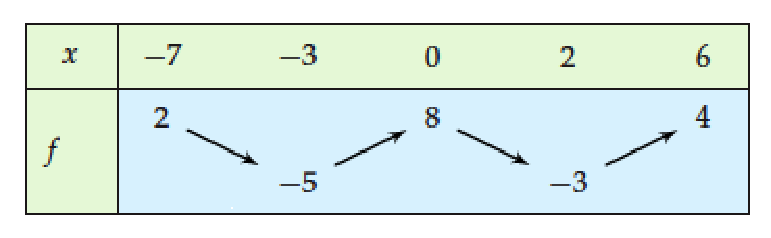
\includegraphics[scale=0.6]{Fonctions/figures/Ex22.eps}
\end{exercice}

\begin{exercice}
Pour chacune des courbes suivantes, établir le tableau
de variations des fonctions représentées.
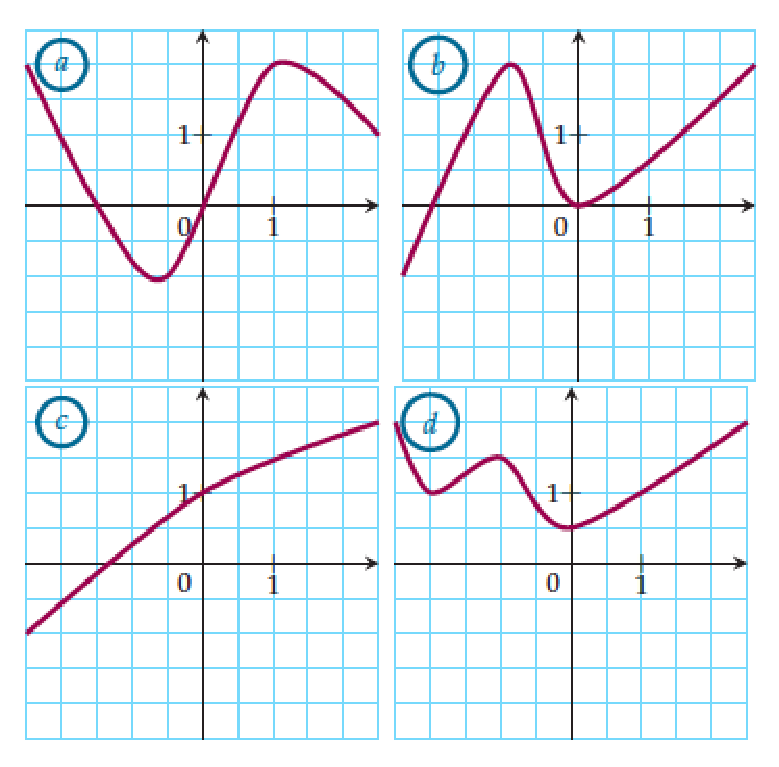
\includegraphics[scale=0.6]{Fonctions/figures/Ex23.eps}
\end{exercice}

\begin{exercice}
Voici le tableau de variations d’une fonction f .
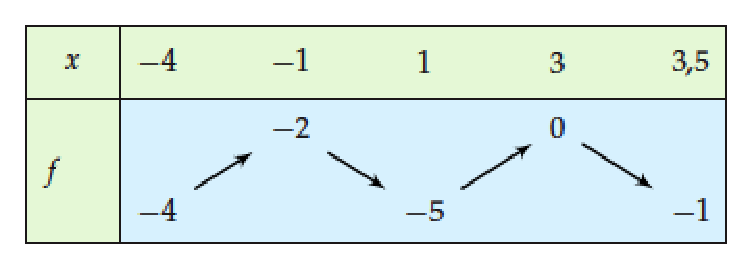
\includegraphics[scale=0.6]{Fonctions/figures/Ex24.eps}
\begin{enumerate}
\item Quel est l’ensemble de définition de la fonction $f$ ?
\item Indiquer le sens de variations de la fonction $f$ .
\item Préciser les extrema éventuels de la fonction $f$
et pour quelle(s) valeur(s) ils sont atteints.
\item Tracer deux courbes différentes susceptibles de représenter
graphiquement la fonction $f$ .
\end{enumerate}
\end{exercice}

\serie{Résolution graphique}

\begin{exercice}
Reprendre les représentations graphiques de l'exercice 19.
\begin{enumerate}
	\item Résoudre l'équation $f(x)=1$;
	\item Résoudre l'équation $g(x)=-1$;
	\item Déterminer sur quel(s) intervalle(s) $f$ est positive ou nulle;
	\item Déterminer sur quel(s) intervalle(s) $f$ est strictement négative;
	\item Déterminer le ou les zéros de $f$;
	\item Déterminer  le ou les zéros de $g$.
\end{enumerate}
\end{exercice}

\begin{exercice}
Voici le tableau de variations d’une fonction $f$ .
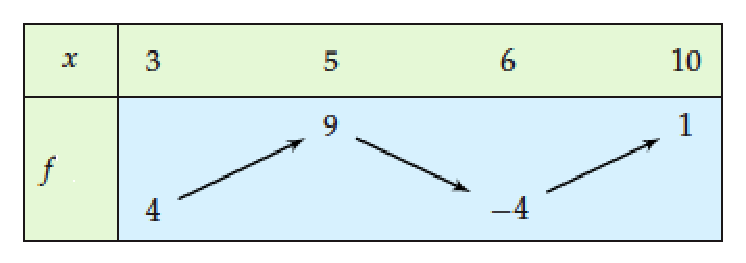
\includegraphics[scale=0.65]{Fonctions/figures/Ex25.eps}
Pour chacune des propositions suivantes, dire si elle est
vraie, fausse ou si on ne peut pas conclure. Justifier.
\begin{enumerate}
\setlength{\columnseprule}{0pt}
\begin{multicols}{2}
\item $f (3) < f (4)$;
\item $f (4, 9) > f (5, 9)$ ;
\item $f (5, 1) < f (5, 9)$;
\item $f (10) > f (3)$;
\end{multicols}
\item $f$ est définie sur [-2; 10] ;
\item 5 est le maximum de $f$ sur [3; 10] ;
\item Le minimum de $f$ est 4 sur [3; 10] ;
\item Si $x\in[3;10]$, $f (x)$ appartient à [-4; 9].
\end{enumerate}
\end{exercice}

\begin{exercice}
On donne le tableau de variations d'une fonction $f$:
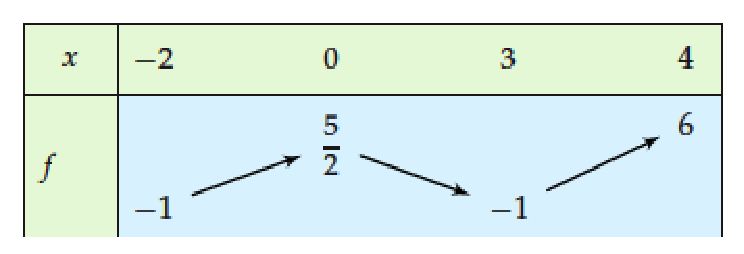
\includegraphics[scale=0.65]{Fonctions/figures/Ex26.eps}
Comparer si possible les nombres suivants.
\setlength{\columnseprule}{0pt}
\begin{multicols}{2}
\begin{enumerate}
\item $f (-2)$ et $f (-1)$;
\item $f\left( \dfrac{1}{3} \right) $ et $f\left( \dfrac{3}{2} \right) $;
\item $f (-1)$ et $f (1)$;
\item $f (3, 6)$ et $f (3, 7)$;
\item $f (1)$ et $f (3, 5)$. 
\end{enumerate}
\end{multicols}
\end{exercice}

\begin{exercice}
Soit $f$ une fonction définie sur [-2; 5] telle que :
\begin{itemize}
\item  $f (-2) = 2$
\item  $f (2) = -3$
\item  $f (5) = 0$
\item $f$ est décroissante sur ]-2; 2[ et croissante sinon ;
\item $f$ admet un minimum en 2 égal à -3.
\end{itemize}
\begin{enumerate}
\item Encadrer $f (x)$ quand :
\begin{enumerate}
\item $x \in ]-2; 2[$
\item $x \in ]3; 4[$
\end{enumerate}
\item Si $x \in [-2; 5]$, que peut-on dire de $f (x)$ ?
\item Quels sont les extrema de $f$ ?
\end{enumerate}
\end{exercice}

\begin{exercice}
Tracer le tableau de signe et le tableau de variation des graphes des fonctions des exercices 1 et 17.
\end{exercice}

\begin{exercice}
Tracer le tableau de signe et le tableau de variation de la fonction $f$ représentée ci-dessous.
\begin{center}
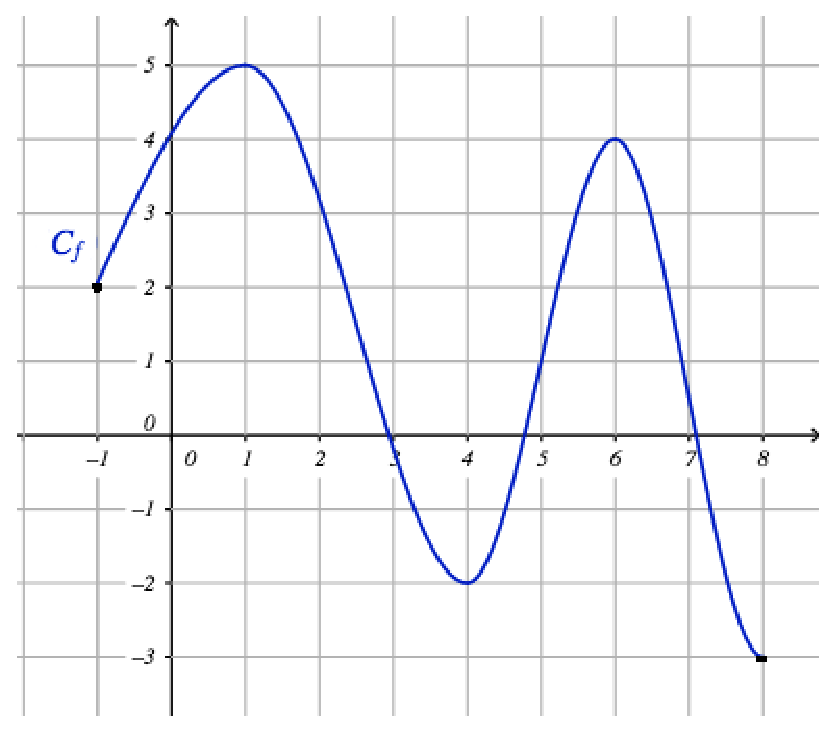
\includegraphics[scale=0.5]{Fonctions/figures/rep8.eps}
\end{center}
\end{exercice}

\begin{exercice}
A l'aide du graphique, répondre aux questions suivantes:

\definecolor{qqqqff}{rgb}{0.,0.,1.}
\definecolor{ffqqqq}{rgb}{1.,0.,0.}
\definecolor{cqcqcq}{rgb}{0.752941176471,0.752941176471,0.752941176471}
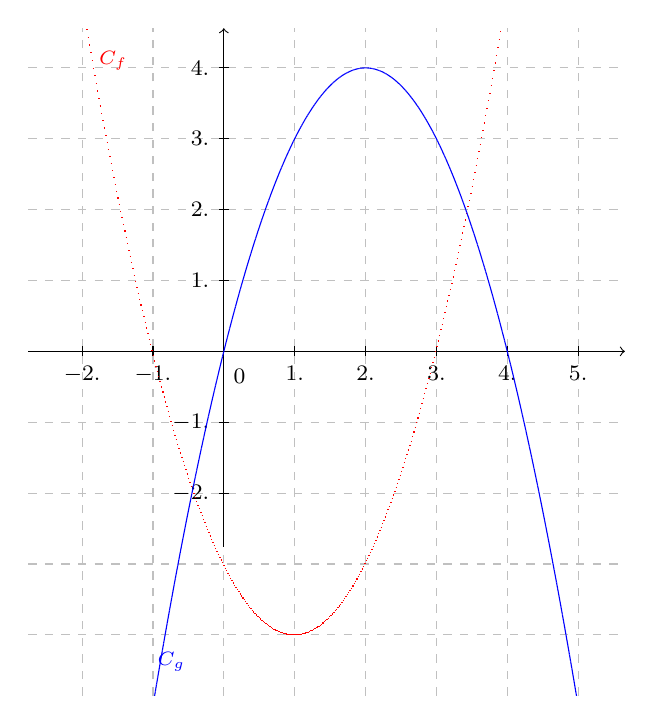
\begin{tikzpicture}[scale=0.9][line cap=round,line join=round,>=triangle 45,x=1.0cm,y=1.0cm]
\draw [color=cqcqcq,dash pattern=on 3pt off 3pt, xstep=1.0cm,ystep=1.0cm] (-2.76,-4.86) grid (5.66,4.56);
\draw[->,color=black] (-2.76,0.) -- (5.66,0.);
\foreach \x in {-2.,-1.,1.,2.,3.,4.,5.}
\draw[shift={(\x,0)},color=black] (0pt,2pt) -- (0pt,-2pt) node[below] {\footnotesize $\x$};
\draw[->,color=black] (0.,-2.76) -- (0.,4.56);
\foreach \y in {-2.,-1.,1.,2.,3.,4.}
\draw[shift={(0,\y)},color=black] (2pt,0pt) -- (-2pt,0pt) node[left] {\footnotesize $\y$};
\draw[color=black] (0pt,-10pt) node[right] {\footnotesize $0$};
\clip(-2.76,-4.86) rectangle (5.66,4.56);
\draw[color=ffqqqq] (-1.9999939600000067,4.885430803890008) -- (-1.9808439751000066,4.885430803890008);
\draw[color=ffqqqq] (-1.9808439751000066,4.771631291586837) -- (-1.9616939902000066,4.771631291586837);
\draw[color=ffqqqq] (-1.9616939902000066,4.658565223127004) -- (-1.9425440053000065,4.658565223127004);
\draw[color=ffqqqq] (-1.9425440053000065,4.546232598510513) -- (-1.9233940204000064,4.546232598510513);
\draw[color=ffqqqq] (-1.9233940204000064,4.434633417737363) -- (-1.9042440355000063,4.434633417737363);
\draw[color=ffqqqq] (-1.9042440355000063,4.323767680807552) -- (-1.8850940506000062,4.323767680807552);
\draw[color=ffqqqq] (-1.8850940506000062,4.213635387721081) -- (-1.8659440657000061,4.213635387721081);
\draw[color=ffqqqq] (-1.8659440657000061,4.104236538477951) -- (-1.846794080800006,4.104236538477951);
\draw[color=ffqqqq] (-1.846794080800006,3.995571133078162) -- (-1.827644095900006,3.995571133078162);
\draw[color=ffqqqq] (-1.827644095900006,3.887639171521714) -- (-1.808494111000006,3.887639171521714);
\draw[color=ffqqqq] (-1.808494111000006,3.780440653808605) -- (-1.7893441261000058,3.780440653808605);
\draw[color=ffqqqq] (-1.7893441261000058,3.673975579938837) -- (-1.7701941412000057,3.673975579938837);
\draw[color=ffqqqq] (-1.7701941412000057,3.5682439499124103) -- (-1.7510441563000056,3.5682439499124103);
\draw[color=ffqqqq] (-1.7510441563000056,3.463245763729323) -- (-1.7318941714000056,3.463245763729323);
\draw[color=ffqqqq] (-1.7318941714000056,3.3589810213895763) -- (-1.7127441865000055,3.3589810213895763);
\draw[color=ffqqqq] (-1.7127441865000055,3.2554497228931703) -- (-1.6935942016000054,3.2554497228931703);
\draw[color=ffqqqq] (-1.6935942016000054,3.152651868240105) -- (-1.6744442167000053,3.152651868240105);
\draw[color=ffqqqq] (-1.6744442167000053,3.05058745743038) -- (-1.6552942318000052,3.05058745743038);
\draw[color=ffqqqq] (-1.6552942318000052,2.9492564904639953) -- (-1.6361442469000052,2.9492564904639953);
\draw[color=ffqqqq] (-1.6361442469000052,2.848658967340951) -- (-1.616994262000005,2.848658967340951);
\draw[color=ffqqqq] (-1.616994262000005,2.748794888061248) -- (-1.597844277100005,2.748794888061248);
\draw[color=ffqqqq] (-1.597844277100005,2.6496642526248846) -- (-1.578694292200005,2.6496642526248846);
\draw[color=ffqqqq] (-1.578694292200005,2.5512670610318615) -- (-1.5595443073000048,2.5512670610318615);
\draw[color=ffqqqq] (-1.5595443073000048,2.453603313282179) -- (-1.5403943224000047,2.453603313282179);
\draw[color=ffqqqq] (-1.5403943224000047,2.3566730093758372) -- (-1.5212443375000047,2.3566730093758372);
\draw[color=ffqqqq] (-1.5212443375000047,2.260476149312836) -- (-1.5020943526000046,2.260476149312836);
\draw[color=ffqqqq] (-1.5020943526000046,2.165012733093175) -- (-1.4829443677000045,2.165012733093175);
\draw[color=ffqqqq] (-1.4829443677000045,2.0702827607168546) -- (-1.4637943828000044,2.0702827607168546);
\draw[color=ffqqqq] (-1.4637943828000044,1.9762862321838748) -- (-1.4446443979000043,1.9762862321838748);
\draw[color=ffqqqq] (-1.4446443979000043,1.8830231474942352) -- (-1.4254944130000042,1.8830231474942352);
\draw[color=ffqqqq] (-1.4254944130000042,1.790493506647936) -- (-1.4063444281000042,1.790493506647936);
\draw[color=ffqqqq] (-1.4063444281000042,1.6986973096449773) -- (-1.387194443200004,1.6986973096449773);
\draw[color=ffqqqq] (-1.387194443200004,1.6076345564853591) -- (-1.368044458300004,1.6076345564853591);
\draw[color=ffqqqq] (-1.368044458300004,1.5173052471690818) -- (-1.348894473400004,1.5173052471690818);
\draw[color=ffqqqq] (-1.348894473400004,1.4277093816961444) -- (-1.3297444885000038,1.4277093816961444);
\draw[color=ffqqqq] (-1.3297444885000038,1.3388469600665476) -- (-1.3105945036000037,1.3388469600665476);
\draw[color=ffqqqq] (-1.3105945036000037,1.2507179822802914) -- (-1.2914445187000037,1.2507179822802914);
\draw[color=ffqqqq] (-1.2914445187000037,1.1633224483373756) -- (-1.2722945338000036,1.1633224483373756);
\draw[color=ffqqqq] (-1.2722945338000036,1.0766603582378003) -- (-1.2531445489000035,1.0766603582378003);
\draw[color=ffqqqq] (-1.2531445489000035,0.9907317119815653) -- (-1.2339945640000034,0.9907317119815653);
\draw[color=ffqqqq] (-1.2339945640000034,0.9055365095686707) -- (-1.2148445791000033,0.9055365095686707);
\draw[color=ffqqqq] (-1.2148445791000033,0.821074750999117) -- (-1.1956945942000032,0.821074750999117);
\draw[color=ffqqqq] (-1.1956945942000032,0.7373464362729034) -- (-1.1765446093000032,0.7373464362729034);
\draw[color=ffqqqq] (-1.1765446093000032,0.6543515653900303) -- (-1.157394624400003,0.6543515653900303);
\draw[color=ffqqqq] (-1.157394624400003,0.5720901383504978) -- (-1.138244639500003,0.5720901383504978);
\draw[color=ffqqqq] (-1.138244639500003,0.4905621551543056) -- (-1.119094654600003,0.4905621551543056);
\draw[color=ffqqqq] (-1.119094654600003,0.40976761580145393) -- (-1.0999446697000028,0.40976761580145393);
\draw[color=ffqqqq] (-1.0999446697000028,0.3297065202919427) -- (-1.0807946848000027,0.3297065202919427);
\draw[color=ffqqqq] (-1.0807946848000027,0.25037886862577197) -- (-1.0616446999000027,0.25037886862577197);
\draw[color=ffqqqq] (-1.0616446999000027,0.17178466080294172) -- (-1.0424947150000026,0.17178466080294172);
\draw[color=ffqqqq] (-1.0424947150000026,0.09392389682345191) -- (-1.0233447301000025,0.09392389682345191);
\draw[color=ffqqqq] (-1.0233447301000025,0.016796576687302556) -- (-1.0041947452000024,0.016796576687302556);
\draw[color=ffqqqq] (-1.0041947452000024,-0.05959729960550589) -- (-0.9850447603000024,-0.05959729960550589);
\draw[color=ffqqqq] (-0.9850447603000024,-0.13525773205497388) -- (-0.9658947754000025,-0.13525773205497388);
\draw[color=ffqqqq] (-0.9658947754000025,-0.21018472066110144) -- (-0.9467447905000025,-0.21018472066110144);
\draw[color=ffqqqq] (-0.9467447905000025,-0.28437826542388855) -- (-0.9275948056000025,-0.28437826542388855);
\draw[color=ffqqqq] (-0.9275948056000025,-0.35783836634333516) -- (-0.9084448207000025,-0.35783836634333516);
\draw[color=ffqqqq] (-0.9084448207000025,-0.4305650234194413) -- (-0.8892948358000026,-0.4305650234194413);
\draw[color=ffqqqq] (-0.8892948358000026,-0.5025582366522071) -- (-0.8701448509000026,-0.5025582366522071);
\draw[color=ffqqqq] (-0.8701448509000026,-0.5738180060416322) -- (-0.8509948660000026,-0.5738180060416322);
\draw[color=ffqqqq] (-0.8509948660000026,-0.6443443315877171) -- (-0.8318448811000027,-0.6443443315877171);
\draw[color=ffqqqq] (-0.8318448811000027,-0.7141372132904615) -- (-0.8126948962000027,-0.7141372132904615);
\draw[color=ffqqqq] (-0.8126948962000027,-0.7831966511498655) -- (-0.7935449113000027,-0.7831966511498655);
\draw[color=ffqqqq] (-0.7935449113000027,-0.8515226451659289) -- (-0.7743949264000027,-0.8515226451659289);
\draw[color=ffqqqq] (-0.7743949264000027,-0.9191151953386518) -- (-0.7552449415000028,-0.9191151953386518);
\draw[color=ffqqqq] (-0.7552449415000028,-0.9859743016680345) -- (-0.7360949566000028,-0.9859743016680345);
\draw[color=ffqqqq] (-0.7360949566000028,-1.0520999641540765) -- (-0.7169449717000028,-1.0520999641540765);
\draw[color=ffqqqq] (-0.7169449717000028,-1.117492182796778) -- (-0.6977949868000028,-1.117492182796778);
\draw[color=ffqqqq] (-0.6977949868000028,-1.1821509575961393) -- (-0.6786450019000029,-1.1821509575961393);
\draw[color=ffqqqq] (-0.6786450019000029,-1.2460762885521601) -- (-0.6594950170000029,-1.2460762885521601);
\draw[color=ffqqqq] (-0.6594950170000029,-1.3092681756648403) -- (-0.6403450321000029,-1.3092681756648403);
\draw[color=ffqqqq] (-0.6403450321000029,-1.3717266189341804) -- (-0.621195047200003,-1.3717266189341804);
\draw[color=ffqqqq] (-0.621195047200003,-1.4334516183601795) -- (-0.602045062300003,-1.4334516183601795);
\draw[color=ffqqqq] (-0.602045062300003,-1.4944431739428385) -- (-0.582895077400003,-1.4944431739428385);
\draw[color=ffqqqq] (-0.582895077400003,-1.554701285682157) -- (-0.563745092500003,-1.554701285682157);
\draw[color=ffqqqq] (-0.563745092500003,-1.614225953578135) -- (-0.5445951076000031,-1.614225953578135);
\draw[color=ffqqqq] (-0.5445951076000031,-1.6730171776307725) -- (-0.5254451227000031,-1.6730171776307725);
\draw[color=ffqqqq] (-0.5254451227000031,-1.7310749578400697) -- (-0.5062951378000031,-1.7310749578400697);
\draw[color=ffqqqq] (-0.5062951378000031,-1.7883992942060267) -- (-0.4871451529000031,-1.7883992942060267);
\draw[color=ffqqqq] (-0.4871451529000031,-1.8449901867286427) -- (-0.46799516800000307,-1.8449901867286427);
\draw[color=ffqqqq] (-0.46799516800000307,-1.9008476354079185) -- (-0.44884518310000304,-1.9008476354079185);
\draw[color=ffqqqq] (-0.44884518310000304,-1.955971640243854) -- (-0.429695198200003,-1.955971640243854);
\draw[color=ffqqqq] (-0.429695198200003,-2.010362201236449) -- (-0.410545213300003,-2.010362201236449);
\draw[color=ffqqqq] (-0.410545213300003,-2.0640193183857036) -- (-0.39139522840000296,-2.0640193183857036);
\draw[color=ffqqqq] (-0.39139522840000296,-2.1169429916916176) -- (-0.37224524350000293,-2.1169429916916176);
\draw[color=ffqqqq] (-0.37224524350000293,-2.1691332211541914) -- (-0.3530952586000029,-2.1691332211541914);
\draw[color=ffqqqq] (-0.3530952586000029,-2.2205900067734246) -- (-0.3339452737000029,-2.2205900067734246);
\draw[color=ffqqqq] (-0.3339452737000029,-2.271313348549317) -- (-0.31479528880000285,-2.271313348549317);
\draw[color=ffqqqq] (-0.31479528880000285,-2.321303246481869) -- (-0.2956453039000028,-2.321303246481869);
\draw[color=ffqqqq] (-0.2956453039000028,-2.3705597005710812) -- (-0.2764953190000028,-2.3705597005710812);
\draw[color=ffqqqq] (-0.2764953190000028,-2.4190827108169524) -- (-0.25734533410000276,-2.4190827108169524);
\draw[color=ffqqqq] (-0.25734533410000276,-2.4668722772194833) -- (-0.23819534920000274,-2.4668722772194833);
\draw[color=ffqqqq] (-0.23819534920000274,-2.513928399778673) -- (-0.2190453643000027,-2.513928399778673);
\draw[color=ffqqqq] (-0.2190453643000027,-2.560251078494524) -- (-0.19989537940000268,-2.560251078494524);
\draw[color=ffqqqq] (-0.19989537940000268,-2.6058403133670334) -- (-0.18074539450000265,-2.6058403133670334);
\draw[color=ffqqqq] (-0.18074539450000265,-2.650696104396202) -- (-0.16159540960000263,-2.650696104396202);
\draw[color=ffqqqq] (-0.16159540960000263,-2.6948184515820306) -- (-0.1424454247000026,-2.6948184515820306);
\draw[color=ffqqqq] (-0.1424454247000026,-2.7382073549245187) -- (-0.12329543980000257,-2.7382073549245187);
\draw[color=ffqqqq] (-0.12329543980000257,-2.7808628144236667) -- (-0.10414545490000254,-2.7808628144236667);
\draw[color=ffqqqq] (-0.10414545490000254,-2.8227848300794736) -- (-0.08499547000000252,-2.8227848300794736);
\draw[color=ffqqqq] (-0.08499547000000252,-2.86397340189194) -- (-0.06584548510000249,-2.86397340189194);
\draw[color=ffqqqq] (-0.06584548510000249,-2.904428529861067) -- (-0.04669550020000247,-2.904428529861067);
\draw[color=ffqqqq] (-0.04669550020000247,-2.9441502139868523) -- (-0.027545515300002446,-2.9441502139868523);
\draw[color=ffqqqq] (-0.027545515300002446,-2.9831384542692976) -- (-0.008395530400002425,-2.9831384542692976);
\draw[color=ffqqqq] (-0.008395530400002425,-3.0213932507084027) -- (0.010754454499997596,-3.0213932507084027);
\draw[color=ffqqqq] (0.010754454499997596,-3.058914603304167) -- (0.029904439399997616,-3.058914603304167);
\draw[color=ffqqqq] (0.029904439399997616,-3.095702512056591) -- (0.04905442429999764,-3.095702512056591);
\draw[color=ffqqqq] (0.04905442429999764,-3.1317569769656743) -- (0.06820440919999765,-3.1317569769656743);
\draw[color=ffqqqq] (0.06820440919999765,-3.167077998031418) -- (0.08735439409999768,-3.167077998031418);
\draw[color=ffqqqq] (0.08735439409999768,-3.2016655752538203) -- (0.1065043789999977,-3.2016655752538203);
\draw[color=ffqqqq] (0.1065043789999977,-3.235519708632882) -- (0.12565436389999773,-3.235519708632882);
\draw[color=ffqqqq] (0.12565436389999773,-3.268640398168604) -- (0.14480434879999776,-3.268640398168604);
\draw[color=ffqqqq] (0.14480434879999776,-3.3010276438609853) -- (0.1639543336999978,-3.3010276438609853);
\draw[color=ffqqqq] (0.1639543336999978,-3.3326814457100267) -- (0.18310431859999782,-3.3326814457100267);
\draw[color=ffqqqq] (0.18310431859999782,-3.3636018037157265) -- (0.20225430349999785,-3.3636018037157265);
\draw[color=ffqqqq] (0.20225430349999785,-3.393788717878086) -- (0.22140428839999787,-3.393788717878086);
\draw[color=ffqqqq] (0.22140428839999787,-3.4232421881971056) -- (0.2405542732999979,-3.4232421881971056);
\draw[color=ffqqqq] (0.2405542732999979,-3.451962214672785) -- (0.25970425819999793,-3.451962214672785);
\draw[color=ffqqqq] (0.25970425819999793,-3.479948797305123) -- (0.27885424309999796,-3.479948797305123);
\draw[color=ffqqqq] (0.27885424309999796,-3.5072019360941207) -- (0.298004227999998,-3.5072019360941207);
\draw[color=ffqqqq] (0.298004227999998,-3.5337216310397785) -- (0.317154212899998,-3.5337216310397785);
\draw[color=ffqqqq] (0.317154212899998,-3.5595078821420962) -- (0.33630419779999804,-3.5595078821420962);
\draw[color=ffqqqq] (0.33630419779999804,-3.584560689401073) -- (0.35545418269999807,-3.584560689401073);
\draw[color=ffqqqq] (0.35545418269999807,-3.608880052816709) -- (0.3746041675999981,-3.608880052816709);
\draw[color=ffqqqq] (0.3746041675999981,-3.6324659723890047) -- (0.3937541524999981,-3.6324659723890047);
\draw[color=ffqqqq] (0.3937541524999981,-3.65531844811796) -- (0.41290413739999815,-3.65531844811796);
\draw[color=ffqqqq] (0.41290413739999815,-3.6774374800035745) -- (0.4320541222999982,-3.6774374800035745);
\draw[color=ffqqqq] (0.4320541222999982,-3.6988230680458485) -- (0.4512041071999982,-3.6988230680458485);
\draw[color=ffqqqq] (0.4512041071999982,-3.7194752122447827) -- (0.47035409209999823,-3.7194752122447827);
\draw[color=ffqqqq] (0.47035409209999823,-3.739393912600377) -- (0.48950407699999826,-3.739393912600377);
\draw[color=ffqqqq] (0.48950407699999826,-3.7585791691126293) -- (0.5086540618999983,-3.7585791691126293);
\draw[color=ffqqqq] (0.5086540618999983,-3.7770309817815417) -- (0.5278040467999983,-3.7770309817815417);
\draw[color=ffqqqq] (0.5278040467999983,-3.7947493506071135) -- (0.5469540316999982,-3.7947493506071135);
\draw[color=ffqqqq] (0.5469540316999982,-3.8117342755893455) -- (0.5661040165999982,-3.8117342755893455);
\draw[color=ffqqqq] (0.5661040165999982,-3.8279857567282365) -- (0.5852540014999982,-3.8279857567282365);
\draw[color=ffqqqq] (0.5852540014999982,-3.8435037940237873) -- (0.6044039863999981,-3.8435037940237873);
\draw[color=ffqqqq] (0.6044039863999981,-3.8582883874759974) -- (0.6235539712999981,-3.8582883874759974);
\draw[color=ffqqqq] (0.6235539712999981,-3.8723395370848666) -- (0.6427039561999981,-3.8723395370848666);
\draw[color=ffqqqq] (0.6427039561999981,-3.8856572428503964) -- (0.6618539410999981,-3.8856572428503964);
\draw[color=ffqqqq] (0.6618539410999981,-3.898241504772585) -- (0.681003925999998,-3.898241504772585);
\draw[color=ffqqqq] (0.681003925999998,-3.9100923228514337) -- (0.700153910899998,-3.9100923228514337);
\draw[color=ffqqqq] (0.700153910899998,-3.921209697086942) -- (0.719303895799998,-3.921209697086942);
\draw[color=ffqqqq] (0.719303895799998,-3.931593627479109) -- (0.738453880699998,-3.931593627479109);
\draw[color=ffqqqq] (0.738453880699998,-3.941244114027936) -- (0.7576038655999979,-3.941244114027936);
\draw[color=ffqqqq] (0.7576038655999979,-3.9501611567334227) -- (0.7767538504999979,-3.9501611567334227);
\draw[color=ffqqqq] (0.7767538504999979,-3.9583447555955686) -- (0.7959038353999979,-3.9583447555955686);
\draw[color=ffqqqq] (0.7959038353999979,-3.9657949106143744) -- (0.8150538202999978,-3.9657949106143744);
\draw[color=ffqqqq] (0.8150538202999978,-3.9725116217898395) -- (0.8342038051999978,-3.9725116217898395);
\draw[color=ffqqqq] (0.8342038051999978,-3.9784948891219645) -- (0.8533537900999978,-3.9784948891219645);
\draw[color=ffqqqq] (0.8533537900999978,-3.9837447126107493) -- (0.8725037749999978,-3.9837447126107493);
\draw[color=ffqqqq] (0.8725037749999978,-3.9882610922561925) -- (0.8916537598999977,-3.9882610922561925);
\draw[color=ffqqqq] (0.8916537598999977,-3.992044028058296) -- (0.9108037447999977,-3.992044028058296);
\draw[color=ffqqqq] (0.9108037447999977,-3.995093520017059) -- (0.9299537296999977,-3.995093520017059);
\draw[color=ffqqqq] (0.9299537296999977,-3.9974095681324813) -- (0.9491037145999976,-3.9974095681324813);
\draw[color=ffqqqq] (0.9491037145999976,-3.9989921724045634) -- (0.9682536994999976,-3.9989921724045634);
\draw[color=ffqqqq] (0.9682536994999976,-3.9998413328333053) -- (0.9874036843999976,-3.9998413328333053);
\draw[color=ffqqqq] (0.9874036843999976,-3.9999570494187067) -- (1.0065536692999977,-3.9999570494187067);
\draw[color=ffqqqq] (1.0065536692999977,-3.999339322160767) -- (1.0257036541999978,-3.999339322160767);
\draw[color=ffqqqq] (1.0257036541999978,-3.9979881510594866) -- (1.0448536390999978,-3.9979881510594866);
\draw[color=ffqqqq] (1.0448536390999978,-3.995903536114867) -- (1.064003623999998,-3.995903536114867);
\draw[color=ffqqqq] (1.064003623999998,-3.9930854773269067) -- (1.083153608899998,-3.9930854773269067);
\draw[color=ffqqqq] (1.083153608899998,-3.989533974695605) -- (1.102303593799998,-3.989533974695605);
\draw[color=ffqqqq] (1.102303593799998,-3.985249028220963) -- (1.1214535786999982,-3.985249028220963);
\draw[color=ffqqqq] (1.1214535786999982,-3.9802306379029813) -- (1.1406035635999983,-3.9802306379029813);
\draw[color=ffqqqq] (1.1406035635999983,-3.974478803741659) -- (1.1597535484999983,-3.974478803741659);
\draw[color=ffqqqq] (1.1597535484999983,-3.9679935257369956) -- (1.1789035333999984,-3.9679935257369956);
\draw[color=ffqqqq] (1.1789035333999984,-3.9607748038889916) -- (1.1980535182999985,-3.9607748038889916);
\draw[color=ffqqqq] (1.1980535182999985,-3.9528226381976483) -- (1.2172035031999986,-3.9528226381976483);
\draw[color=ffqqqq] (1.2172035031999986,-3.944137028662964) -- (1.2363534880999987,-3.944137028662964);
\draw[color=ffqqqq] (1.2363534880999987,-3.934717975284939) -- (1.2555034729999988,-3.934717975284939);
\draw[color=ffqqqq] (1.2555034729999988,-3.924565478063573) -- (1.2746534578999988,-3.924565478063573);
\draw[color=ffqqqq] (1.2746534578999988,-3.9136795369988677) -- (1.293803442799999,-3.9136795369988677);
\draw[color=ffqqqq] (1.293803442799999,-3.902060152090822) -- (1.312953427699999,-3.902060152090822);
\draw[color=ffqqqq] (1.312953427699999,-3.889707323339435) -- (1.332103412599999,-3.889707323339435);
\draw[color=ffqqqq] (1.332103412599999,-3.876621050744707) -- (1.3512533974999992,-3.876621050744707);
\draw[color=ffqqqq] (1.3512533974999992,-3.86280133430664) -- (1.3704033823999993,-3.86280133430664);
\draw[color=ffqqqq] (1.3704033823999993,-3.8482481740252323) -- (1.3895533672999993,-3.8482481740252323);
\draw[color=ffqqqq] (1.3895533672999993,-3.8329615699004833) -- (1.4087033521999994,-3.8329615699004833);
\draw[color=ffqqqq] (1.4087033521999994,-3.8169415219323937) -- (1.4278533370999995,-3.8169415219323937);
\draw[color=ffqqqq] (1.4278533370999995,-3.8001880301209647) -- (1.4470033219999996,-3.8001880301209647);
\draw[color=ffqqqq] (1.4470033219999996,-3.782701094466195) -- (1.4661533068999997,-3.782701094466195);
\draw[color=ffqqqq] (1.4661533068999997,-3.764480714968084) -- (1.4853032917999998,-3.764480714968084);
\draw[color=ffqqqq] (1.4853032917999998,-3.745526891626633) -- (1.5044532766999998,-3.745526891626633);
\draw[color=ffqqqq] (1.5044532766999998,-3.725839624441842) -- (1.5236032616,-3.725839624441842);
\draw[color=ffqqqq] (1.5236032616,-3.7054189134137108) -- (1.5427532465,-3.7054189134137108);
\draw[color=ffqqqq] (1.5427532465,-3.684264758542238) -- (1.5619032314,-3.684264758542238);
\draw[color=ffqqqq] (1.5619032314,-3.662377159827425) -- (1.5810532163000002,-3.662377159827425);
\draw[color=ffqqqq] (1.5810532163000002,-3.639756117269272) -- (1.6002032012000003,-3.639756117269272);
\draw[color=ffqqqq] (1.6002032012000003,-3.6164016308677787) -- (1.6193531861000003,-3.6164016308677787);
\draw[color=ffqqqq] (1.6193531861000003,-3.5923137006229444) -- (1.6385031710000004,-3.5923137006229444);
\draw[color=ffqqqq] (1.6385031710000004,-3.567492326534769) -- (1.6576531559000005,-3.567492326534769);
\draw[color=ffqqqq] (1.6576531559000005,-3.5419375086032545) -- (1.6768031408000006,-3.5419375086032545);
\draw[color=ffqqqq] (1.6768031408000006,-3.5156492468283993) -- (1.6959531257000007,-3.5156492468283993);
\draw[color=ffqqqq] (1.6959531257000007,-3.488627541210203) -- (1.7151031106000008,-3.488627541210203);
\draw[color=ffqqqq] (1.7151031106000008,-3.4608723917486666) -- (1.7342530955000008,-3.4608723917486666);
\draw[color=ffqqqq] (1.7342530955000008,-3.43238379844379) -- (1.753403080400001,-3.43238379844379);
\draw[color=ffqqqq] (1.753403080400001,-3.4031617612955727) -- (1.772553065300001,-3.4031617612955727);
\draw[color=ffqqqq] (1.772553065300001,-3.3732062803040144) -- (1.791703050200001,-3.3732062803040144);
\draw[color=ffqqqq] (1.791703050200001,-3.342517355469116) -- (1.8108530351000012,-3.342517355469116);
\draw[color=ffqqqq] (1.8108530351000012,-3.3110949867908777) -- (1.8300030200000013,-3.3110949867908777);
\draw[color=ffqqqq] (1.8300030200000013,-3.2789391742692984) -- (1.8491530049000013,-3.2789391742692984);
\draw[color=ffqqqq] (1.8491530049000013,-3.2460499179043785) -- (1.8683029898000014,-3.2460499179043785);
\draw[color=ffqqqq] (1.8683029898000014,-3.2124272176961184) -- (1.8874529747000015,-3.2124272176961184);
\draw[color=ffqqqq] (1.8874529747000015,-3.1780710736445177) -- (1.9066029596000016,-3.1780710736445177);
\draw[color=ffqqqq] (1.9066029596000016,-3.1429814857495773) -- (1.9257529445000017,-3.1429814857495773);
\draw[color=ffqqqq] (1.9257529445000017,-3.1071584540112953) -- (1.9449029294000018,-3.1071584540112953);
\draw[color=ffqqqq] (1.9449029294000018,-3.070601978429673) -- (1.9640529143000018,-3.070601978429673);
\draw[color=ffqqqq] (1.9640529143000018,-3.033312059004711) -- (1.983202899200002,-3.033312059004711);
\draw[color=ffqqqq] (1.983202899200002,-2.9952886957364084) -- (2.002352884100002,-2.9952886957364084);
\draw[color=ffqqqq] (2.002352884100002,-2.9565318886247653) -- (2.0215028690000016,-2.9565318886247653);
\draw[color=ffqqqq] (2.0215028690000016,-2.917041637669782) -- (2.0406528539000015,-2.917041637669782);
\draw[color=ffqqqq] (2.0406528539000015,-2.876817942871458) -- (2.0598028388000014,-2.876817942871458);
\draw[color=ffqqqq] (2.0598028388000014,-2.835860804229794) -- (2.0789528237000012,-2.835860804229794);
\draw[color=ffqqqq] (2.0789528237000012,-2.7941702217447895) -- (2.098102808600001,-2.7941702217447895);
\draw[color=ffqqqq] (2.098102808600001,-2.751746195416444) -- (2.117252793500001,-2.751746195416444);
\draw[color=ffqqqq] (2.117252793500001,-2.7085887252447587) -- (2.136402778400001,-2.7085887252447587);
\draw[color=ffqqqq] (2.136402778400001,-2.6646978112297326) -- (2.1555527633000007,-2.6646978112297326);
\draw[color=ffqqqq] (2.1555527633000007,-2.6200734533713663) -- (2.1747027482000005,-2.6200734533713663);
\draw[color=ffqqqq] (2.1747027482000005,-2.5747156516696594) -- (2.1938527331000004,-2.5747156516696594);
\draw[color=ffqqqq] (2.1938527331000004,-2.528624406124612) -- (2.2130027180000003,-2.528624406124612);
\draw[color=ffqqqq] (2.2130027180000003,-2.4817997167362242) -- (2.2321527029,-2.4817997167362242);
\draw[color=ffqqqq] (2.2321527029,-2.434241583504496) -- (2.2513026878,-2.434241583504496);
\draw[color=ffqqqq] (2.2513026878,-2.385950006429427) -- (2.2704526727,-2.385950006429427);
\draw[color=ffqqqq] (2.2704526727,-2.336924985511018) -- (2.2896026575999997,-2.336924985511018);
\draw[color=ffqqqq] (2.2896026575999997,-2.287166520749268) -- (2.3087526424999996,-2.287166520749268);
\draw[color=ffqqqq] (2.3087526424999996,-2.2366746121441783) -- (2.3279026273999994,-2.2366746121441783);
\draw[color=ffqqqq] (2.3279026273999994,-2.1854492596957478) -- (2.3470526122999993,-2.1854492596957478);
\draw[color=ffqqqq] (2.3470526122999993,-2.133490463403977) -- (2.366202597199999,-2.133490463403977);
\draw[color=ffqqqq] (2.366202597199999,-2.0807982232688653) -- (2.385352582099999,-2.0807982232688653);
\draw[color=ffqqqq] (2.385352582099999,-2.027372539290414) -- (2.404502566999999,-2.027372539290414);
\draw[color=ffqqqq] (2.404502566999999,-1.9732134114686215) -- (2.4236525518999987,-1.9732134114686215);
\draw[color=ffqqqq] (2.4236525518999987,-1.9183208398034888) -- (2.4428025367999986,-1.9183208398034888);
\draw[color=ffqqqq] (2.4428025367999986,-1.8626948242950156) -- (2.4619525216999985,-1.8626948242950156);
\draw[color=ffqqqq] (2.4619525216999985,-1.806335364943202) -- (2.4811025065999983,-1.806335364943202);
\draw[color=ffqqqq] (2.4811025065999983,-1.749242461748048) -- (2.500252491499998,-1.749242461748048);
\draw[color=ffqqqq] (2.500252491499998,-1.6914161147095534) -- (2.519402476399998,-1.6914161147095534);
\draw[color=ffqqqq] (2.519402476399998,-1.6328563238277185) -- (2.538552461299998,-1.6328563238277185);
\draw[color=ffqqqq] (2.538552461299998,-1.5735630891025432) -- (2.5577024461999978,-1.5735630891025432);
\draw[color=ffqqqq] (2.5577024461999978,-1.5135364105340272) -- (2.5768524310999976,-1.5135364105340272);
\draw[color=ffqqqq] (2.5768524310999976,-1.452776288122171) -- (2.5960024159999975,-1.452776288122171);
\draw[color=ffqqqq] (2.5960024159999975,-1.3912827218669743) -- (2.6151524008999973,-1.3912827218669743);
\draw[color=ffqqqq] (2.6151524008999973,-1.3290557117684372) -- (2.634302385799997,-1.3290557117684372);
\draw[color=ffqqqq] (2.634302385799997,-1.2660952578265594) -- (2.653452370699997,-1.2660952578265594);
\draw[color=ffqqqq] (2.653452370699997,-1.2024013600413415) -- (2.672602355599997,-1.2024013600413415);
\draw[color=ffqqqq] (2.672602355599997,-1.137974018412783) -- (2.691752340499997,-1.137974018412783);
\draw[color=ffqqqq] (2.691752340499997,-1.072813232940884) -- (2.7109023253999966,-1.072813232940884);
\draw[color=ffqqqq] (2.7109023253999966,-1.0069190036256446) -- (2.7300523102999965,-1.0069190036256446);
\draw[color=ffqqqq] (2.7300523102999965,-0.9402913304670647) -- (2.7492022951999964,-0.9402913304670647);
\draw[color=ffqqqq] (2.7492022951999964,-0.8729302134651444) -- (2.7683522800999962,-0.8729302134651444);
\draw[color=ffqqqq] (2.7683522800999962,-0.8048356526198838) -- (2.787502264999996,-0.8048356526198838);
\draw[color=ffqqqq] (2.787502264999996,-0.7360076479312826) -- (2.806652249899996,-0.7360076479312826);
\draw[color=ffqqqq] (2.806652249899996,-0.6664461993993409) -- (2.825802234799996,-0.6664461993993409);
\draw[color=ffqqqq] (2.825802234799996,-0.5961513070240588) -- (2.8449522196999957,-0.5961513070240588);
\draw[color=ffqqqq] (2.8449522196999957,-0.5251229708054364) -- (2.8641022045999955,-0.5251229708054364);
\draw[color=ffqqqq] (2.8641022045999955,-0.4533611907434734) -- (2.8832521894999954,-0.4533611907434734);
\draw[color=ffqqqq] (2.8832521894999954,-0.38086596683817003) -- (2.9024021743999953,-0.38086596683817003);
\draw[color=ffqqqq] (2.9024021743999953,-0.3076372990895262) -- (2.921552159299995,-0.3076372990895262);
\draw[color=ffqqqq] (2.921552159299995,-0.23367518749754188) -- (2.940702144199995,-0.23367518749754188);
\draw[color=ffqqqq] (2.940702144199995,-0.15897963206221713) -- (2.959852129099995,-0.15897963206221713);
\draw[color=ffqqqq] (2.959852129099995,-0.08355063278355196) -- (2.9790021139999947,-0.08355063278355196);
\draw[color=ffqqqq] (2.9790021139999947,-0.007388189661546332) -- (2.9981520988999946,-0.007388189661546332);
\draw[color=ffqqqq] (2.9981520988999946,0.06950769730379974) -- (3.0173020837999944,0.06950769730379974);
\draw[color=ffqqqq] (3.0173020837999944,0.14713702811248625) -- (3.0364520686999943,0.14713702811248625);
\draw[color=ffqqqq] (3.0364520686999943,0.22549980276451323) -- (3.055602053599994,0.22549980276451323);
\draw[color=ffqqqq] (3.055602053599994,0.30459602125988067) -- (3.074752038499994,0.30459602125988067);
\draw[color=ffqqqq] (3.074752038499994,0.3844256835985885) -- (3.093902023399994,0.3844256835985885);
\draw[color=ffqqqq] (3.093902023399994,0.46498878978063674) -- (3.1130520082999937,0.46498878978063674);
\draw[color=ffqqqq] (3.1130520082999937,0.5462853398060256) -- (3.1322019931999936,0.5462853398060256);
\draw[color=ffqqqq] (3.1322019931999936,0.6283153336747548) -- (3.1513519780999935,0.6283153336747548);
\draw[color=ffqqqq] (3.1513519780999935,0.7110787713868244) -- (3.1705019629999933,0.7110787713868244);
\draw[color=ffqqqq] (3.1705019629999933,0.7945756529422343) -- (3.189651947899993,0.7945756529422343);
\draw[color=ffqqqq] (3.189651947899993,0.878805978340985) -- (3.208801932799993,0.878805978340985);
\draw[color=ffqqqq] (3.208801932799993,0.963769747583076) -- (3.227951917699993,0.963769747583076);
\draw[color=ffqqqq] (3.227951917699993,1.0494669606685074) -- (3.2471019025999928,1.0494669606685074);
\draw[color=ffqqqq] (3.2471019025999928,1.135897617597279) -- (3.2662518874999926,1.135897617597279);
\draw[color=ffqqqq] (3.2662518874999926,1.2230617183693915) -- (3.2854018723999925,1.2230617183693915);
\draw[color=ffqqqq] (3.2854018723999925,1.3109592629848443) -- (3.3045518572999923,1.3109592629848443);
\draw[color=ffqqqq] (3.3045518572999923,1.3995902514436376) -- (3.323701842199992,1.3995902514436376);
\draw[color=ffqqqq] (3.323701842199992,1.488954683745771) -- (3.342851827099992,1.488954683745771);
\draw[color=ffqqqq] (3.342851827099992,1.5790525598912453) -- (3.362001811999992,1.5790525598912453);
\draw[color=ffqqqq] (3.362001811999992,1.66988387988006) -- (3.381151796899992,1.66988387988006);
\draw[color=ffqqqq] (3.381151796899992,1.7614486437122148) -- (3.4003017817999917,1.7614486437122148);
\draw[color=ffqqqq] (3.4003017817999917,1.85374685138771) -- (3.4194517666999915,1.85374685138771);
\draw[color=ffqqqq] (3.4194517666999915,1.946778502906546) -- (3.4386017515999914,1.946778502906546);
\draw[color=ffqqqq] (3.4386017515999914,2.0405435982687226) -- (3.4577517364999912,2.0405435982687226);
\draw[color=ffqqqq] (3.4577517364999912,2.135042137474239) -- (3.476901721399991,2.135042137474239);
\draw[color=ffqqqq] (3.476901721399991,2.230274120523096) -- (3.496051706299991,2.230274120523096);
\draw[color=ffqqqq] (3.496051706299991,2.326239547415294) -- (3.515201691199991,2.326239547415294);
\draw[color=ffqqqq] (3.515201691199991,2.4229384181508324) -- (3.5343516760999907,2.4229384181508324);
\draw[color=ffqqqq] (3.5343516760999907,2.5203707327297105) -- (3.5535016609999905,2.5203707327297105);
\draw[color=ffqqqq] (3.5535016609999905,2.6185364911519295) -- (3.5726516458999904,2.6185364911519295);
\draw[color=ffqqqq] (3.5726516458999904,2.7174356934174893) -- (3.5918016307999903,2.7174356934174893);
\draw[color=ffqqqq] (3.5918016307999903,2.817068339526389) -- (3.61095161569999,2.817068339526389);
\draw[color=ffqqqq] (3.61095161569999,2.917434429478629) -- (3.63010160059999,2.917434429478629);
\draw[color=ffqqqq] (3.63010160059999,3.01853396327421) -- (3.64925158549999,3.01853396327421);
\draw[color=ffqqqq] (3.64925158549999,3.120366940913131) -- (3.6684015703999897,3.120366940913131);
\draw[color=ffqqqq] (3.6684015703999897,3.222933362395393) -- (3.6875515552999896,3.222933362395393);
\draw[color=ffqqqq] (3.6875515552999896,3.326233227720995) -- (3.7067015401999894,3.326233227720995);
\draw[color=ffqqqq] (3.7067015401999894,3.4302665368899374) -- (3.7258515250999893,3.4302665368899374);
\draw[color=ffqqqq] (3.7258515250999893,3.5350332899022208) -- (3.745001509999989,3.5350332899022208);
\draw[color=ffqqqq] (3.745001509999989,3.6405334867578443) -- (3.764151494899989,3.6405334867578443);
\draw[color=ffqqqq] (3.764151494899989,3.746767127456808) -- (3.783301479799989,3.746767127456808);
\draw[color=ffqqqq] (3.783301479799989,3.853734211999112) -- (3.8024514646999887,3.853734211999112);
\draw[color=ffqqqq] (3.8024514646999887,3.961434740384757) -- (3.8216014495999886,3.961434740384757);
\draw[color=ffqqqq] (3.8216014495999886,4.069868712613743) -- (3.8407514344999885,4.069868712613743);
\draw[color=ffqqqq] (3.8407514344999885,4.179036128686068) -- (3.8599014193999883,4.179036128686068);
\draw[color=ffqqqq] (3.8599014193999883,4.2889369886017334) -- (3.879051404299988,4.2889369886017334);
\draw[color=ffqqqq] (3.879051404299988,4.399571292360741) -- (3.898201389199988,4.399571292360741);
\draw[color=ffqqqq] (3.898201389199988,4.5109390399630875) -- (3.917351374099988,4.5109390399630875);
\draw[color=ffqqqq] (3.917351374099988,4.623040231408775) -- (3.9365013589999878,4.623040231408775);
\draw[color=ffqqqq] (3.9365013589999878,4.735874866697802) -- (3.9556513438999876,4.735874866697802);
\draw[color=ffqqqq] (3.9556513438999876,4.849442945830171) -- (3.9748013287999875,4.849442945830171);
\draw[color=ffqqqq] (3.9748013287999875,4.9637444688058805) -- (3.9939513136999873,4.9637444688058805);
\draw[color=ffqqqq] (3.9939513136999873,5.078779435624929) -- (4.013101298599987,5.078779435624929);
\draw[color=ffqqqq] (4.013101298599987,5.194547846287322) -- (4.0322512834999875,5.194547846287322);
\draw[color=ffqqqq] (4.0322512834999875,5.311049700793054) -- (4.051401268399988,5.311049700793054);
\draw[color=ffqqqq] (4.051401268399988,5.428284999142128) -- (4.070551253299988,5.428284999142128);
\draw[color=ffqqqq] (4.070551253299988,5.546253741334541) -- (4.089701238199988,5.546253741334541);
\draw[color=ffqqqq] (4.089701238199988,5.664955927370296) -- (4.108851223099989,5.664955927370296);
\draw[color=ffqqqq] (4.108851223099989,5.784391557249391) -- (4.128001207999989,5.784391557249391);
\draw[color=ffqqqq] (4.128001207999989,5.904560630971826) -- (4.147151192899989,5.904560630971826);
\draw[color=ffqqqq] (4.147151192899989,6.025463148537602) -- (4.16630117779999,6.025463148537602);
\draw[color=ffqqqq] (4.16630117779999,6.147099109946718) -- (4.18545116269999,6.147099109946718);
\draw[color=ffqqqq] (4.18545116269999,6.269468515199175) -- (4.20460114759999,6.269468515199175);
\draw[color=ffqqqq] (4.20460114759999,6.392571364294971) -- (4.223751132499991,6.392571364294971);
\draw[color=ffqqqq] (4.223751132499991,6.516407657234109) -- (4.242901117399991,6.516407657234109);
\draw[color=ffqqqq] (4.242901117399991,6.640977394016588) -- (4.262051102299991,6.640977394016588);
\draw[color=ffqqqq] (4.262051102299991,6.766280574642406) -- (4.2812010871999915,6.766280574642406);
\draw[color=ffqqqq] (4.2812010871999915,6.892317199111565) -- (4.300351072099992,6.892317199111565);
\draw[color=ffqqqq] (4.300351072099992,7.019087267424065) -- (4.319501056999992,7.019087267424065);
\draw[color=ffqqqq] (4.319501056999992,7.146590779579904) -- (4.338651041899992,7.146590779579904);
\draw[color=ffqqqq] (4.338651041899992,7.274827735579085) -- (4.357801026799993,7.274827735579085);
\draw[color=ffqqqq] (4.357801026799993,7.4037981354216065) -- (4.376951011699993,7.4037981354216065);
\draw[color=ffqqqq] (4.376951011699993,7.533501979107468) -- (4.396100996599993,7.533501979107468);
\draw[color=ffqqqq] (4.396100996599993,7.66393926663667) -- (4.415250981499994,7.66393926663667);
\draw[color=ffqqqq] (4.415250981499994,7.795109998009212) -- (4.434400966399994,7.795109998009212);
\draw[color=ffqqqq] (4.434400966399994,7.927014173225095) -- (4.453550951299994,7.927014173225095);
\draw[color=ffqqqq] (4.453550951299994,8.059651792284319) -- (4.4727009361999945,8.059651792284319);
\draw[color=ffqqqq] (4.4727009361999945,8.193022855186882) -- (4.491850921099995,8.193022855186882);
\draw[color=ffqqqq] (4.491850921099995,8.327127361932787) -- (4.511000905999995,8.327127361932787);
\draw[color=ffqqqq] (4.511000905999995,8.461965312522032) -- (4.5301508908999955,8.461965312522032);
\draw[color=ffqqqq] (4.5301508908999955,8.597536706954617) -- (4.549300875799996,8.597536706954617);
\draw[color=ffqqqq] (4.549300875799996,8.733841545230543) -- (4.568450860699996,8.733841545230543);
\draw[color=ffqqqq] (4.568450860699996,8.870879827349809) -- (4.587600845599996,8.870879827349809);
\draw[color=ffqqqq] (4.587600845599996,9.008651553312415) -- (4.606750830499997,9.008651553312415);
\draw[color=ffqqqq] (4.606750830499997,9.147156723118362) -- (4.625900815399997,9.147156723118362);
\draw[color=ffqqqq] (4.625900815399997,9.28639533676765) -- (4.645050800299997,9.28639533676765);
\draw[color=ffqqqq] (4.645050800299997,9.426367394260279) -- (4.664200785199998,9.426367394260279);
\draw[color=ffqqqq] (4.664200785199998,9.567072895596247) -- (4.683350770099998,9.567072895596247);
\draw[color=ffqqqq] (4.683350770099998,9.708511840775557) -- (4.702500754999998,9.708511840775557);
\draw[color=ffqqqq] (4.702500754999998,9.850684229798206) -- (4.7216507398999985,9.850684229798206);
\draw[color=ffqqqq] (4.7216507398999985,9.993590062664197) -- (4.740800724799999,9.993590062664197);
\draw[color=ffqqqq] (4.740800724799999,10.137229339373526) -- (4.759950709699999,10.137229339373526);
\draw[color=ffqqqq] (4.759950709699999,10.281602059926199) -- (4.779100694599999,10.281602059926199);
\draw[color=ffqqqq] (4.779100694599999,10.42670822432221) -- (4.7982506795,10.42670822432221);
\draw[color=ffqqqq] (4.7982506795,10.572547832561561) -- (4.8174006644,10.572547832561561);
\draw[color=ffqqqq] (4.8174006644,10.719120884644255) -- (4.8365506493,10.719120884644255);
\draw[color=ffqqqq] (4.8365506493,10.866427380570288) -- (4.855700634200001,10.866427380570288);
\draw[color=ffqqqq] (4.855700634200001,11.01446732033966) -- (4.874850619100001,11.01446732033966);
\draw[color=ffqqqq] (4.874850619100001,11.163240703952374) -- (4.894000604000001,11.163240703952374);
\draw[color=ffqqqq] (4.894000604000001,11.312747531408428) -- (4.913150588900002,11.312747531408428);
\draw[color=ffqqqq] (4.913150588900002,11.462987802707824) -- (4.932300573800002,11.462987802707824);
\draw[color=ffqqqq] (4.932300573800002,11.613961517850559) -- (4.951450558700002,11.613961517850559);
\draw[color=ffqqqq] (4.951450558700002,11.765668676836635) -- (4.9706005436000025,11.765668676836635);
\draw[color=ffqqqq] (4.9706005436000025,11.918109279666051) -- (4.989750528500003,11.918109279666051);
\draw[color=ffqqqq] (4.989750528500003,12.071283326338808) -- (5.008900513400003,12.071283326338808);
\draw[color=ffqqqq] (5.008900513400003,12.225190816854905) -- (5.028050498300003,12.225190816854905);
\draw[color=ffqqqq] (5.028050498300003,12.379831751214343) -- (5.047200483200004,12.379831751214343);
\draw[color=ffqqqq] (5.047200483200004,12.535206129417121) -- (5.066350468100004,12.535206129417121);
\draw[color=ffqqqq] (5.066350468100004,12.69131395146324) -- (5.085500453000004,12.69131395146324);
\draw[color=ffqqqq] (5.085500453000004,12.8481552173527) -- (5.104650437900005,12.8481552173527);
\draw[color=ffqqqq] (5.104650437900005,13.005729927085499) -- (5.123800422800005,13.005729927085499);
\draw[color=ffqqqq] (5.123800422800005,13.164038080661639) -- (5.142950407700005,13.164038080661639);
\draw[color=ffqqqq] (5.142950407700005,13.32307967808112) -- (5.1621003926000055,13.32307967808112);
\draw[color=ffqqqq] (5.1621003926000055,13.48285471934394) -- (5.181250377500006,13.48285471934394);
\draw[color=ffqqqq] (5.181250377500006,13.643363204450102) -- (5.200400362400006,13.643363204450102);
\draw[color=ffqqqq] (5.200400362400006,13.804605133399605) -- (5.219550347300006,13.804605133399605);
\draw[color=ffqqqq] (5.219550347300006,13.966580506192448) -- (5.238700332200007,13.966580506192448);
\draw[color=ffqqqq] (5.238700332200007,14.129289322828631) -- (5.257850317100007,14.129289322828631);
\draw[color=ffqqqq] (5.257850317100007,14.292731583308154) -- (5.277000302000007,14.292731583308154);
\draw[color=ffqqqq] (5.277000302000007,14.456907287631019) -- (5.296150286900008,14.456907287631019);
\draw[color=ffqqqq] (5.296150286900008,14.621816435797223) -- (5.315300271800008,14.621816435797223);
\draw[color=ffqqqq] (5.315300271800008,14.787459027806767) -- (5.334450256700008,14.787459027806767);
\draw[color=ffqqqq] (5.334450256700008,14.953835063659653) -- (5.353600241600009,14.953835063659653);
\draw[color=ffqqqq] (5.353600241600009,15.12094454335588) -- (5.372750226500009,15.12094454335588);
\draw[color=ffqqqq] (5.372750226500009,15.288787466895446) -- (5.391900211400009,15.288787466895446);
\draw[color=ffqqqq] (5.391900211400009,15.457363834278352) -- (5.4110501963000095,15.457363834278352);
\draw[color=ffqqqq] (5.4110501963000095,15.6266736455046) -- (5.43020018120001,15.6266736455046);
\draw[color=ffqqqq] (5.43020018120001,15.796716900574188) -- (5.44935016610001,15.796716900574188);
\draw[color=ffqqqq] (5.44935016610001,15.967493599487115) -- (5.46850015100001,15.967493599487115);
\draw[color=ffqqqq] (5.46850015100001,16.139003742243386) -- (5.487650135900011,16.139003742243386);
\draw[color=ffqqqq] (5.487650135900011,16.311247328842995) -- (5.506800120800011,16.311247328842995);
\draw[color=ffqqqq] (5.506800120800011,16.484224359285943) -- (5.525950105700011,16.484224359285943);
\draw[color=ffqqqq] (5.525950105700011,16.657934833572234) -- (5.545100090600012,16.657934833572234);
\draw[color=ffqqqq] (5.545100090600012,16.832378751701864) -- (5.564250075500012,16.832378751701864);
\draw[color=ffqqqq] (5.564250075500012,17.007556113674834) -- (5.583400060400012,17.007556113674834);
\draw[color=ffqqqq] (5.583400060400012,17.18346691949115) -- (5.6025500453000125,17.18346691949115);
\draw[color=ffqqqq] (5.6025500453000125,17.360111169150798) -- (5.621700030200013,17.360111169150798);
\draw[color=ffqqqq] (5.621700030200013,17.53748886265379) -- (5.640850015100013,17.53748886265379);
;
\draw[color=qqqqff] (-0.9999926600000019,-4.999955960053888) -- (-0.9833426783500019,-4.900333536464563);
\draw[color=qqqqff] (-0.9833426783500019,-4.900333536464563) -- (-0.9666926967000019,-4.801265556653129);
\draw[color=qqqqff] (-0.9666926967000019,-4.801265556653129) -- (-0.9500427150500019,-4.702752020619587);
\draw[color=qqqqff] (-0.9500427150500019,-4.702752020619587) -- (-0.933392733400002,-4.604792928363935);
\draw[color=qqqqff] (-0.933392733400002,-4.604792928363935) -- (-0.916742751750002,-4.5073882798861735);
\draw[color=qqqqff] (-0.916742751750002,-4.5073882798861735) -- (-0.900092770100002,-4.410538075186302);
\draw[color=qqqqff] (-0.900092770100002,-4.410538075186302) -- (-0.883442788450002,-4.314242314264323);
\draw[color=qqqqff] (-0.883442788450002,-4.314242314264323) -- (-0.866792806800002,-4.218500997120234);
\draw[color=qqqqff] (-0.866792806800002,-4.218500997120234) -- (-0.8501428251500021,-4.123314123754035);
\draw[color=qqqqff] (-0.8501428251500021,-4.123314123754035) -- (-0.8334928435000021,-4.028681694165726);
\draw[color=qqqqff] (-0.8334928435000021,-4.028681694165726) -- (-0.8168428618500021,-3.93460370835531);
\draw[color=qqqqff] (-0.8168428618500021,-3.93460370835531) -- (-0.8001928802000021,-3.8410801663227843);
\draw[color=qqqqff] (-0.8001928802000021,-3.8410801663227843) -- (-0.7835428985500021,-3.7481110680681473);
\draw[color=qqqqff] (-0.7835428985500021,-3.7481110680681473) -- (-0.7668929169000022,-3.6556964135914014);
\draw[color=qqqqff] (-0.7668929169000022,-3.6556964135914014) -- (-0.7502429352500022,-3.5638362028925474);
\draw[color=qqqqff] (-0.7502429352500022,-3.5638362028925474) -- (-0.7335929536000022,-3.4725304359715845);
\draw[color=qqqqff] (-0.7335929536000022,-3.4725304359715845) -- (-0.7169429719500022,-3.381779112828511);
\draw[color=qqqqff] (-0.7169429719500022,-3.381779112828511) -- (-0.7002929903000022,-3.2915822334633273);
\draw[color=qqqqff] (-0.7002929903000022,-3.2915822334633273) -- (-0.6836430086500023,-3.201939797876036);
\draw[color=qqqqff] (-0.6836430086500023,-3.201939797876036) -- (-0.6669930270000023,-3.1128518060666353);
\draw[color=qqqqff] (-0.6669930270000023,-3.1128518060666353) -- (-0.6503430453500023,-3.0243182580351244);
\draw[color=qqqqff] (-0.6503430453500023,-3.0243182580351244) -- (-0.6336930637000023,-2.9363391537815042);
\draw[color=qqqqff] (-0.6336930637000023,-2.9363391537815042) -- (-0.6170430820500024,-2.848914493305775);
\draw[color=qqqqff] (-0.6170430820500024,-2.848914493305775) -- (-0.6003931004000024,-2.7620442766079374);
\draw[color=qqqqff] (-0.6003931004000024,-2.7620442766079374) -- (-0.5837431187500024,-2.6757285036879885);
\draw[color=qqqqff] (-0.5837431187500024,-2.6757285036879885) -- (-0.5670931371000024,-2.589967174545931);
\draw[color=qqqqff] (-0.5670931371000024,-2.589967174545931) -- (-0.5504431554500024,-2.5047602891817653);
\draw[color=qqqqff] (-0.5504431554500024,-2.5047602891817653) -- (-0.5337931738000025,-2.4201078475954905);
\draw[color=qqqqff] (-0.5337931738000025,-2.4201078475954905) -- (-0.5171431921500025,-2.3360098497871045);
\draw[color=qqqqff] (-0.5171431921500025,-2.3360098497871045) -- (-0.5004932105000025,-2.252466295756609);
\draw[color=qqqqff] (-0.5004932105000025,-2.252466295756609) -- (-0.48384322885000247,-2.169477185504006);
\draw[color=qqqqff] (-0.48384322885000247,-2.169477185504006) -- (-0.46719324720000244,-2.0870425190292923);
\draw[color=qqqqff] (-0.46719324720000244,-2.0870425190292923) -- (-0.4505432655500024,-2.005162296332469);
\draw[color=qqqqff] (-0.4505432655500024,-2.005162296332469) -- (-0.43389328390000237,-1.9238365174135381);
\draw[color=qqqqff] (-0.43389328390000237,-1.9238365174135381) -- (-0.41724330225000233,-1.8430651822724962);
\draw[color=qqqqff] (-0.41724330225000233,-1.8430651822724962) -- (-0.4005933206000023,-1.7628482909093455);
\draw[color=qqqqff] (-0.4005933206000023,-1.7628482909093455) -- (-0.38394333895000227,-1.6831858433240854);
\draw[color=qqqqff] (-0.38394333895000227,-1.6831858433240854) -- (-0.36729335730000223,-1.6040778395167155);
\draw[color=qqqqff] (-0.36729335730000223,-1.6040778395167155) -- (-0.3506433756500022,-1.5255242794872377);
\draw[color=qqqqff] (-0.3506433756500022,-1.5255242794872377) -- (-0.33399339400000216,-1.4475251632356492);
\draw[color=qqqqff] (-0.33399339400000216,-1.4475251632356492) -- (-0.31734341235000213,-1.3700804907619517);
\draw[color=qqqqff] (-0.31734341235000213,-1.3700804907619517) -- (-0.3006934307000021,-1.293190262066146);
\draw[color=qqqqff] (-0.3006934307000021,-1.293190262066146) -- (-0.28404344905000206,-1.2168544771482297);
\draw[color=qqqqff] (-0.28404344905000206,-1.2168544771482297) -- (-0.267393467400002,-1.141073136008204);
\draw[color=qqqqff] (-0.267393467400002,-1.141073136008204) -- (-0.250743485750002,-1.0658462386460692);
\draw[color=qqqqff] (-0.250743485750002,-1.0658462386460692) -- (-0.234093504100002,-0.991173785061826);
\draw[color=qqqqff] (-0.234093504100002,-0.991173785061826) -- (-0.21744352245000198,-0.9170557752554724);
\draw[color=qqqqff] (-0.21744352245000198,-0.9170557752554724) -- (-0.20079354080000197,-0.8434922092270096);
\draw[color=qqqqff] (-0.20079354080000197,-0.8434922092270096) -- (-0.18414355915000197,-0.7704830869764383);
\draw[color=qqqqff] (-0.18414355915000197,-0.7704830869764383) -- (-0.16749357750000196,-0.6980284085037569);
\draw[color=qqqqff] (-0.16749357750000196,-0.6980284085037569) -- (-0.15084359585000195,-0.6261281738089661);
\draw[color=qqqqff] (-0.15084359585000195,-0.6261281738089661) -- (-0.13419361420000195,-0.5547823828920668);
\draw[color=qqqqff] (-0.13419361420000195,-0.5547823828920668) -- (-0.11754363255000194,-0.4839910357530574);
\draw[color=qqqqff] (-0.11754363255000194,-0.4839910357530574) -- (-0.10089365090000194,-0.41375413239193953);
\draw[color=qqqqff] (-0.10089365090000194,-0.41375413239193953) -- (-0.08424366925000193,-0.3440716728087114);
\draw[color=qqqqff] (-0.08424366925000193,-0.3440716728087114) -- (-0.06759368760000192,-0.27494365700337403);
\draw[color=qqqqff] (-0.06759368760000192,-0.27494365700337403) -- (-0.050943705950001916,-0.20637008497592815);
\draw[color=qqqqff] (-0.050943705950001916,-0.20637008497592815) -- (-0.03429372430000191,-0.13835095672637207);
\draw[color=qqqqff] (-0.03429372430000191,-0.13835095672637207) -- (-0.0176437426500019,-0.07088627225470666);
\draw[color=qqqqff] (-0.0176437426500019,-0.07088627225470666) -- (-9.9376100000189E-4,-0.003976031560932824);
\draw[color=qqqqff] (-9.9376100000189E-4,-0.003976031560932824) -- (0.01565622064999812,0.06237976535495123);
\draw[color=qqqqff] (0.01565622064999812,0.06237976535495123) -- (0.03230620229999813,0.12818111849294417);
\draw[color=qqqqff] (0.03230620229999813,0.12818111849294417) -- (0.048956183949998136,0.19342802785304644);
\draw[color=qqqqff] (0.048956183949998136,0.19342802785304644) -- (0.06560616559999814,0.25812049343525806);
\draw[color=qqqqff] (0.06560616559999814,0.25812049343525806) -- (0.08225614724999815,0.3222585152395794);
\draw[color=qqqqff] (0.08225614724999815,0.3222585152395794) -- (0.09890612889999816,0.3858420932660096);
\draw[color=qqqqff] (0.09890612889999816,0.3858420932660096) -- (0.11555611054999816,0.44887122751454916);
\draw[color=qqqqff] (0.11555611054999816,0.44887122751454916) -- (0.13220609219999818,0.5113459179851981);
\draw[color=qqqqff] (0.13220609219999818,0.5113459179851981) -- (0.1488560738499982,0.5732661646779567);
\draw[color=qqqqff] (0.1488560738499982,0.5732661646779567) -- (0.1655060554999982,0.6346319675928244);
\draw[color=qqqqff] (0.1655060554999982,0.6346319675928244) -- (0.1821560371499982,0.6954433267298011);
\draw[color=qqqqff] (0.1821560371499982,0.6954433267298011) -- (0.1988060187999982,0.7557002420888878);
\draw[color=qqqqff] (0.1988060187999982,0.7557002420888878) -- (0.21545600044999821,0.8154027136700833);
\draw[color=qqqqff] (0.21545600044999821,0.8154027136700833) -- (0.23210598209999822,0.8745507414733882);
\draw[color=qqqqff] (0.23210598209999822,0.8745507414733882) -- (0.24875596374999823,0.9331443254988024);
\draw[color=qqqqff] (0.24875596374999823,0.9331443254988024) -- (0.26540594539999823,0.9911834657463259);
\draw[color=qqqqff] (0.26540594539999823,0.9911834657463259) -- (0.28205592704999827,1.048668162215959);
\draw[color=qqqqff] (0.28205592704999827,1.048668162215959) -- (0.2987059086999983,1.1055984149077016);
\draw[color=qqqqff] (0.2987059086999983,1.1055984149077016) -- (0.31535589034999834,1.1619742238215531);
\draw[color=qqqqff] (0.31535589034999834,1.1619742238215531) -- (0.33200587199999837,1.217795588957514);
\draw[color=qqqqff] (0.33200587199999837,1.217795588957514) -- (0.3486558536499984,1.2730625103155844);
\draw[color=qqqqff] (0.3486558536499984,1.2730625103155844) -- (0.36530583529999844,1.3277749878957645);
\draw[color=qqqqff] (0.36530583529999844,1.3277749878957645) -- (0.3819558169499985,1.3819330216980532);
\draw[color=qqqqff] (0.3819558169499985,1.3819330216980532) -- (0.3986057985999985,1.4355366117224513);
\draw[color=qqqqff] (0.3986057985999985,1.4355366117224513) -- (0.41525578024999854,1.488585757968959);
\draw[color=qqqqff] (0.41525578024999854,1.488585757968959) -- (0.4319057618999986,1.5410804604375763);
\draw[color=qqqqff] (0.4319057618999986,1.5410804604375763) -- (0.4485557435499986,1.5930207191283023);
\draw[color=qqqqff] (0.4485557435499986,1.5930207191283023) -- (0.46520572519999864,1.6444065340411376);
\draw[color=qqqqff] (0.46520572519999864,1.6444065340411376) -- (0.4818557068499987,1.6952379051760829);
\draw[color=qqqqff] (0.4818557068499987,1.6952379051760829) -- (0.4985056884999987,1.745514832533137);
\draw[color=qqqqff] (0.4985056884999987,1.745514832533137) -- (0.5151556701499987,1.7952373161123008);
\draw[color=qqqqff] (0.5151556701499987,1.7952373161123008) -- (0.5318056517999987,1.8444053559135734);
\draw[color=qqqqff] (0.5318056517999987,1.8444053559135734) -- (0.5484556334499987,1.8930189519369554);
\draw[color=qqqqff] (0.5484556334499987,1.8930189519369554) -- (0.5651056150999987,1.941078104182447);
\draw[color=qqqqff] (0.5651056150999987,1.941078104182447) -- (0.5817555967499987,1.9885828126500475);
\draw[color=qqqqff] (0.5817555967499987,1.9885828126500475) -- (0.5984055783999986,2.0355330773397577);
\draw[color=qqqqff] (0.5984055783999986,2.0355330773397577) -- (0.6150555600499986,2.081928898251577);
\draw[color=qqqqff] (0.6150555600499986,2.081928898251577) -- (0.6317055416999986,2.1277702753855054);
\draw[color=qqqqff] (0.6317055416999986,2.1277702753855054) -- (0.6483555233499986,2.1730572087415436);
\draw[color=qqqqff] (0.6483555233499986,2.1730572087415436) -- (0.6650055049999986,2.217789698319691);
\draw[color=qqqqff] (0.6650055049999986,2.217789698319691) -- (0.6816554866499985,2.2619677441199477);
\draw[color=qqqqff] (0.6816554866499985,2.2619677441199477) -- (0.6983054682999985,2.305591346142314);
\draw[color=qqqqff] (0.6983054682999985,2.305591346142314) -- (0.7149554499499985,2.3486605043867894);
\draw[color=qqqqff] (0.7149554499499985,2.3486605043867894) -- (0.7316054315999985,2.3911752188533737);
\draw[color=qqqqff] (0.7316054315999985,2.3911752188533737) -- (0.7482554132499984,2.433135489542068);
\draw[color=qqqqff] (0.7482554132499984,2.433135489542068) -- (0.7649053948999984,2.474541316452871);
\draw[color=qqqqff] (0.7649053948999984,2.474541316452871) -- (0.7815553765499984,2.515392699585784);
\draw[color=qqqqff] (0.7815553765499984,2.515392699585784) -- (0.7982053581999984,2.5556896389408057);
\draw[color=qqqqff] (0.7982053581999984,2.5556896389408057) -- (0.8148553398499984,2.595432134517937);
\draw[color=qqqqff] (0.8148553398499984,2.595432134517937) -- (0.8315053214999983,2.634620186317178);
\draw[color=qqqqff] (0.8315053214999983,2.634620186317178) -- (0.8481553031499983,2.6732537943385277);
\draw[color=qqqqff] (0.8481553031499983,2.6732537943385277) -- (0.8648052847999983,2.711332958581987);
\draw[color=qqqqff] (0.8648052847999983,2.711332958581987) -- (0.8814552664499983,2.7488576790475556);
\draw[color=qqqqff] (0.8814552664499983,2.7488576790475556) -- (0.8981052480999983,2.7858279557352335);
\draw[color=qqqqff] (0.8981052480999983,2.7858279557352335) -- (0.9147552297499982,2.822243788645021);
\draw[color=qqqqff] (0.9147552297499982,2.822243788645021) -- (0.9314052113999982,2.8581051777769173);
\draw[color=qqqqff] (0.9314052113999982,2.8581051777769173) -- (0.9480551930499982,2.8934121231309233);
\draw[color=qqqqff] (0.9480551930499982,2.8934121231309233) -- (0.9647051746999982,2.9281646247070388);
\draw[color=qqqqff] (0.9647051746999982,2.9281646247070388) -- (0.9813551563499981,2.9623626825052636);
\draw[color=qqqqff] (0.9813551563499981,2.9623626825052636) -- (0.9980051379999981,2.9960062965255974);
\draw[color=qqqqff] (0.9980051379999981,2.9960062965255974) -- (1.0146551196499982,3.0290954667680405);
\draw[color=qqqqff] (1.0146551196499982,3.0290954667680405) -- (1.0313051012999983,3.0616301932325936);
\draw[color=qqqqff] (1.0313051012999983,3.0616301932325936) -- (1.0479550829499984,3.0936104759192555);
\draw[color=qqqqff] (1.0479550829499984,3.0936104759192555) -- (1.0646050645999985,3.125036314828027);
\draw[color=qqqqff] (1.0646050645999985,3.125036314828027) -- (1.0812550462499986,3.1559077099589077);
\draw[color=qqqqff] (1.0812550462499986,3.1559077099589077) -- (1.0979050278999987,3.186224661311898);
\draw[color=qqqqff] (1.0979050278999987,3.186224661311898) -- (1.1145550095499988,3.215987168886997);
\draw[color=qqqqff] (1.1145550095499988,3.215987168886997) -- (1.1312049911999988,3.245195232684206);
\draw[color=qqqqff] (1.1312049911999988,3.245195232684206) -- (1.147854972849999,3.273848852703524);
\draw[color=qqqqff] (1.147854972849999,3.273848852703524) -- (1.164504954499999,3.301948028944951);
\draw[color=qqqqff] (1.164504954499999,3.301948028944951) -- (1.1811549361499991,3.329492761408488);
\draw[color=qqqqff] (1.1811549361499991,3.329492761408488) -- (1.1978049177999992,3.356483050094134);
\draw[color=qqqqff] (1.1978049177999992,3.356483050094134) -- (1.2144548994499993,3.382918895001889);
\draw[color=qqqqff] (1.2144548994499993,3.382918895001889) -- (1.2311048810999994,3.408800296131754);
\draw[color=qqqqff] (1.2311048810999994,3.408800296131754) -- (1.2477548627499995,3.434127253483728);
\draw[color=qqqqff] (1.2477548627499995,3.434127253483728) -- (1.2644048443999996,3.458899767057811);
\draw[color=qqqqff] (1.2644048443999996,3.458899767057811) -- (1.2810548260499997,3.483117836854004);
\draw[color=qqqqff] (1.2810548260499997,3.483117836854004) -- (1.2977048076999997,3.5067814628723055);
\draw[color=qqqqff] (1.2977048076999997,3.5067814628723055) -- (1.3143547893499998,3.529890645112717);
\draw[color=qqqqff] (1.3143547893499998,3.529890645112717) -- (1.331004771,3.5524453835752374);
\draw[color=qqqqff] (1.331004771,3.5524453835752374) -- (1.34765475265,3.5744456782598673);
\draw[color=qqqqff] (1.34765475265,3.5744456782598673) -- (1.3643047343,3.5958915291666065);
\draw[color=qqqqff] (1.3643047343,3.5958915291666065) -- (1.3809547159500002,3.616782936295455);
\draw[color=qqqqff] (1.3809547159500002,3.616782936295455) -- (1.3976046976000003,3.6371198996464127);
\draw[color=qqqqff] (1.3976046976000003,3.6371198996464127) -- (1.4142546792500004,3.65690241921948);
\draw[color=qqqqff] (1.4142546792500004,3.65690241921948) -- (1.4309046609000005,3.6761304950146565);
\draw[color=qqqqff] (1.4309046609000005,3.6761304950146565) -- (1.4475546425500005,3.6948041270319423);
\draw[color=qqqqff] (1.4475546425500005,3.6948041270319423) -- (1.4642046242000006,3.7129233152713375);
\draw[color=qqqqff] (1.4642046242000006,3.7129233152713375) -- (1.4808546058500007,3.730488059732842);
\draw[color=qqqqff] (1.4808546058500007,3.730488059732842) -- (1.4975045875000008,3.7474983604164556);
\draw[color=qqqqff] (1.4975045875000008,3.7474983604164556) -- (1.514154569150001,3.763954217322179);
\draw[color=qqqqff] (1.514154569150001,3.763954217322179) -- (1.530804550800001,3.7798556304500113);
\draw[color=qqqqff] (1.530804550800001,3.7798556304500113) -- (1.547454532450001,3.795202599799953);
\draw[color=qqqqff] (1.547454532450001,3.795202599799953) -- (1.5641045141000012,3.809995125372004);
\draw[color=qqqqff] (1.5641045141000012,3.809995125372004) -- (1.5807544957500013,3.824233207166164);
\draw[color=qqqqff] (1.5807544957500013,3.824233207166164) -- (1.5974044774000014,3.837916845182434);
\draw[color=qqqqff] (1.5974044774000014,3.837916845182434) -- (1.6140544590500014,3.851046039420813);
\draw[color=qqqqff] (1.6140544590500014,3.851046039420813) -- (1.6307044407000015,3.8636207898813013);
\draw[color=qqqqff] (1.6307044407000015,3.8636207898813013) -- (1.6473544223500016,3.875641096563899);
\draw[color=qqqqff] (1.6473544223500016,3.875641096563899) -- (1.6640044040000017,3.887106959468606);
\draw[color=qqqqff] (1.6640044040000017,3.887106959468606) -- (1.6806543856500018,3.898018378595422);
\draw[color=qqqqff] (1.6806543856500018,3.898018378595422) -- (1.697304367300002,3.908375353944348);
\draw[color=qqqqff] (1.697304367300002,3.908375353944348) -- (1.713954348950002,3.918177885515383);
\draw[color=qqqqff] (1.713954348950002,3.918177885515383) -- (1.730604330600002,3.927425973308527);
\draw[color=qqqqff] (1.730604330600002,3.927425973308527) -- (1.7472543122500022,3.9361196173237807);
\draw[color=qqqqff] (1.7472543122500022,3.9361196173237807) -- (1.7639042939000023,3.9442588175611433);
\draw[color=qqqqff] (1.7639042939000023,3.9442588175611433) -- (1.7805542755500023,3.9518435740206157);
\draw[color=qqqqff] (1.7805542755500023,3.9518435740206157) -- (1.7972042572000024,3.958873886702197);
\draw[color=qqqqff] (1.7972042572000024,3.958873886702197) -- (1.8138542388500025,3.965349755605888);
\draw[color=qqqqff] (1.8138542388500025,3.965349755605888) -- (1.8305042205000026,3.971271180731688);
\draw[color=qqqqff] (1.8305042205000026,3.971271180731688) -- (1.8471542021500027,3.9766381620795976);
\draw[color=qqqqff] (1.8471542021500027,3.9766381620795976) -- (1.8638041838000028,3.9814506996496166);
\draw[color=qqqqff] (1.8638041838000028,3.9814506996496166) -- (1.8804541654500029,3.9857087934417446);
\draw[color=qqqqff] (1.8804541654500029,3.9857087934417446) -- (1.897104147100003,3.9894124434559823);
\draw[color=qqqqff] (1.897104147100003,3.9894124434559823) -- (1.913754128750003,3.992561649692329);
\draw[color=qqqqff] (1.913754128750003,3.992561649692329) -- (1.9304041104000031,3.995156412150785);
\draw[color=qqqqff] (1.9304041104000031,3.995156412150785) -- (1.9470540920500032,3.9971967308313503);
\draw[color=qqqqff] (1.9470540920500032,3.9971967308313503) -- (1.9637040737000033,3.9986826057340252);
\draw[color=qqqqff] (1.9637040737000033,3.9986826057340252) -- (1.9803540553500034,3.999614036858809);
\draw[color=qqqqff] (1.9803540553500034,3.999614036858809) -- (1.9970040370000035,3.999991024205703);
\draw[color=qqqqff] (1.9970040370000035,3.999991024205703) -- (2.0136540186500036,3.9998135677747055);
\draw[color=qqqqff] (2.0136540186500036,3.9998135677747055) -- (2.0303040003000037,3.999081667565817);
\draw[color=qqqqff] (2.0303040003000037,3.999081667565817) -- (2.0469539819500038,3.9977953235790387);
\draw[color=qqqqff] (2.0469539819500038,3.9977953235790387) -- (2.063603963600004,3.9959545358143695);
\draw[color=qqqqff] (2.063603963600004,3.9959545358143695) -- (2.080253945250004,3.9935593042718094);
\draw[color=qqqqff] (2.080253945250004,3.9935593042718094) -- (2.096903926900004,3.9906096289513586);
\draw[color=qqqqff] (2.096903926900004,3.9906096289513586) -- (2.113553908550004,3.9871055098530173);
\draw[color=qqqqff] (2.113553908550004,3.9871055098530173) -- (2.1302038902000042,3.9830469469767853);
\draw[color=qqqqff] (2.1302038902000042,3.9830469469767853) -- (2.1468538718500043,3.9784339403226627);
\draw[color=qqqqff] (2.1468538718500043,3.9784339403226627) -- (2.1635038535000044,3.973266489890649);
\draw[color=qqqqff] (2.1635038535000044,3.973266489890649) -- (2.1801538351500045,3.967544595680745);
\draw[color=qqqqff] (2.1801538351500045,3.967544595680745) -- (2.1968038168000046,3.96126825769295);
\draw[color=qqqqff] (2.1968038168000046,3.96126825769295) -- (2.2134537984500047,3.9544374759272647);
\draw[color=qqqqff] (2.2134537984500047,3.9544374759272647) -- (2.2301037801000048,3.9470522503836887);
\draw[color=qqqqff] (2.2301037801000048,3.9470522503836887) -- (2.246753761750005,3.939112581062222);
\draw[color=qqqqff] (2.246753761750005,3.939112581062222) -- (2.263403743400005,3.9306184679628644);
\draw[color=qqqqff] (2.263403743400005,3.9306184679628644) -- (2.280053725050005,3.921569911085616);
\draw[color=qqqqff] (2.280053725050005,3.921569911085616) -- (2.296703706700005,3.9119669104304773);
\draw[color=qqqqff] (2.296703706700005,3.9119669104304773) -- (2.313353688350005,3.901809465997448);
\draw[color=qqqqff] (2.313353688350005,3.901809465997448) -- (2.3300036700000053,3.8910975777865278);
\draw[color=qqqqff] (2.3300036700000053,3.8910975777865278) -- (2.3466536516500054,3.8798312457977167);
\draw[color=qqqqff] (2.3466536516500054,3.8798312457977167) -- (2.3633036333000055,3.868010470031015);
\draw[color=qqqqff] (2.3633036333000055,3.868010470031015) -- (2.3799536149500056,3.855635250486423);
\draw[color=qqqqff] (2.3799536149500056,3.855635250486423) -- (2.3966035966000057,3.84270558716394);
\draw[color=qqqqff] (2.3966035966000057,3.84270558716394) -- (2.4132535782500057,3.829221480063566);
\draw[color=qqqqff] (2.4132535782500057,3.829221480063566) -- (2.429903559900006,3.815182929185302);
\draw[color=qqqqff] (2.429903559900006,3.815182929185302) -- (2.446553541550006,3.800589934529147);
\draw[color=qqqqff] (2.446553541550006,3.800589934529147) -- (2.463203523200006,3.7854424960951016);
\draw[color=qqqqff] (2.463203523200006,3.7854424960951016) -- (2.479853504850006,3.7697406138831653);
\draw[color=qqqqff] (2.479853504850006,3.7697406138831653) -- (2.496503486500006,3.7534842878933383);
\draw[color=qqqqff] (2.496503486500006,3.7534842878933383) -- (2.5131534681500063,3.7366735181256203);
\draw[color=qqqqff] (2.5131534681500063,3.7366735181256203) -- (2.5298034498000064,3.719308304580012);
\draw[color=qqqqff] (2.5298034498000064,3.719308304580012) -- (2.5464534314500065,3.701388647256513);
\draw[color=qqqqff] (2.5464534314500065,3.701388647256513) -- (2.5631034131000066,3.682914546155123);
\draw[color=qqqqff] (2.5631034131000066,3.682914546155123) -- (2.5797533947500066,3.663886001275843);
\draw[color=qqqqff] (2.5797533947500066,3.663886001275843) -- (2.5964033764000067,3.6443030126186717);
\draw[color=qqqqff] (2.5964033764000067,3.6443030126186717) -- (2.613053358050007,3.62416558018361);
\draw[color=qqqqff] (2.613053358050007,3.62416558018361) -- (2.629703339700007,3.603473703970658);
\draw[color=qqqqff] (2.629703339700007,3.603473703970658) -- (2.646353321350007,3.5822273839798147);
\draw[color=qqqqff] (2.646353321350007,3.5822273839798147) -- (2.663003303000007,3.560426620211081);
\draw[color=qqqqff] (2.663003303000007,3.560426620211081) -- (2.679653284650007,3.5380714126644563);
\draw[color=qqqqff] (2.679653284650007,3.5380714126644563) -- (2.6963032663000073,3.5151617613399413);
\draw[color=qqqqff] (2.6963032663000073,3.5151617613399413) -- (2.7129532479500074,3.491697666237535);
\draw[color=qqqqff] (2.7129532479500074,3.491697666237535) -- (2.7296032296000075,3.467679127357239);
\draw[color=qqqqff] (2.7296032296000075,3.467679127357239) -- (2.7462532112500075,3.4431061446990516);
\draw[color=qqqqff] (2.7462532112500075,3.4431061446990516) -- (2.7629031929000076,3.4179787182629737);
\draw[color=qqqqff] (2.7629031929000076,3.4179787182629737) -- (2.7795531745500077,3.392296848049005);
\draw[color=qqqqff] (2.7795531745500077,3.392296848049005) -- (2.796203156200008,3.366060534057146);
\draw[color=qqqqff] (2.796203156200008,3.366060534057146) -- (2.812853137850008,3.339269776287396);
\draw[color=qqqqff] (2.812853137850008,3.339269776287396) -- (2.829503119500008,3.3119245747397557);
\draw[color=qqqqff] (2.829503119500008,3.3119245747397557) -- (2.846153101150008,3.2840249294142243);
\draw[color=qqqqff] (2.846153101150008,3.2840249294142243) -- (2.862803082800008,3.2555708403108023);
\draw[color=qqqqff] (2.862803082800008,3.2555708403108023) -- (2.8794530644500083,3.22656230742949);
\draw[color=qqqqff] (2.8794530644500083,3.22656230742949) -- (2.8961030461000083,3.196999330770286);
\draw[color=qqqqff] (2.8961030461000083,3.196999330770286) -- (2.9127530277500084,3.1668819103331924);
\draw[color=qqqqff] (2.9127530277500084,3.1668819103331924) -- (2.9294030094000085,3.1362100461182076);
\draw[color=qqqqff] (2.9294030094000085,3.1362100461182076) -- (2.9460529910500086,3.1049837381253322);
\draw[color=qqqqff] (2.9460529910500086,3.1049837381253322) -- (2.9627029727000087,3.0732029863545662);
\draw[color=qqqqff] (2.9627029727000087,3.0732029863545662) -- (2.979352954350009,3.0408677908059096);
\draw[color=qqqqff] (2.979352954350009,3.0408677908059096) -- (2.996002936000009,3.007978151479362);
\draw[color=qqqqff] (2.996002936000009,3.007978151479362) -- (3.012652917650009,2.974534068374924);
\draw[color=qqqqff] (3.012652917650009,2.974534068374924) -- (3.029302899300009,2.9405355414925953);
\draw[color=qqqqff] (3.029302899300009,2.9405355414925953) -- (3.045952880950009,2.905982570832376);
\draw[color=qqqqff] (3.045952880950009,2.905982570832376) -- (3.0626028626000092,2.870875156394266);
\draw[color=qqqqff] (3.0626028626000092,2.870875156394266) -- (3.0792528442500093,2.835213298178265);
\draw[color=qqqqff] (3.0792528442500093,2.835213298178265) -- (3.0959028259000094,2.7989969961843735);
\draw[color=qqqqff] (3.0959028259000094,2.7989969961843735) -- (3.1125528075500095,2.7622262504125916);
\draw[color=qqqqff] (3.1125528075500095,2.7622262504125916) -- (3.1292027892000096,2.7249010608629187);
\draw[color=qqqqff] (3.1292027892000096,2.7249010608629187) -- (3.1458527708500097,2.6870214275353552);
\draw[color=qqqqff] (3.1458527708500097,2.6870214275353552) -- (3.16250275250001,2.648587350429901);
\draw[color=qqqqff] (3.16250275250001,2.648587350429901) -- (3.17915273415001,2.609598829546556);
\draw[color=qqqqff] (3.17915273415001,2.609598829546556) -- (3.19580271580001,2.5700558648853207);
\draw[color=qqqqff] (3.19580271580001,2.5700558648853207) -- (3.21245269745001,2.5299584564461943);
\draw[color=qqqqff] (3.21245269745001,2.5299584564461943) -- (3.22910267910001,2.4893066042291774);
\draw[color=qqqqff] (3.22910267910001,2.4893066042291774) -- (3.2457526607500102,2.44810030823427);
\draw[color=qqqqff] (3.2457526607500102,2.44810030823427) -- (3.2624026424000103,2.4063395684614717);
\draw[color=qqqqff] (3.2624026424000103,2.4063395684614717) -- (3.2790526240500104,2.364024384910783);
\draw[color=qqqqff] (3.2790526240500104,2.364024384910783) -- (3.2957026057000105,2.321154757582203);
\draw[color=qqqqff] (3.2957026057000105,2.321154757582203) -- (3.3123525873500106,2.2777306864757327);
\draw[color=qqqqff] (3.3123525873500106,2.2777306864757327) -- (3.3290025690000107,2.2337521715913717);
\draw[color=qqqqff] (3.3290025690000107,2.2337521715913717) -- (3.3456525506500108,2.18921921292912);
\draw[color=qqqqff] (3.3456525506500108,2.18921921292912) -- (3.362302532300011,2.144131810488978);
\draw[color=qqqqff] (3.362302532300011,2.144131810488978) -- (3.378952513950011,2.0984899642709447);
\draw[color=qqqqff] (3.378952513950011,2.0984899642709447) -- (3.395602495600011,2.0522936742750213);
\draw[color=qqqqff] (3.395602495600011,2.0522936742750213) -- (3.412252477250011,2.005542940501207);
\draw[color=qqqqff] (3.412252477250011,2.005542940501207) -- (3.428902458900011,1.9582377629495018);
\draw[color=qqqqff] (3.428902458900011,1.9582377629495018) -- (3.4455524405500113,1.910378141619906);
\draw[color=qqqqff] (3.4455524405500113,1.910378141619906) -- (3.4622024222000114,1.8619640765124197);
\draw[color=qqqqff] (3.4622024222000114,1.8619640765124197) -- (3.4788524038500115,1.8129955676270426);
\draw[color=qqqqff] (3.4788524038500115,1.8129955676270426) -- (3.4955023855000116,1.7634726149637747);
\draw[color=qqqqff] (3.4955023855000116,1.7634726149637747) -- (3.5121523671500117,1.7133952185226162);
\draw[color=qqqqff] (3.5121523671500117,1.7133952185226162) -- (3.5288023488000118,1.6627633783035671);
\draw[color=qqqqff] (3.5288023488000118,1.6627633783035671) -- (3.545452330450012,1.6115770943066274);
\draw[color=qqqqff] (3.545452330450012,1.6115770943066274) -- (3.562102312100012,1.559836366531797);
\draw[color=qqqqff] (3.562102312100012,1.559836366531797) -- (3.578752293750012,1.5075411949790758);
\draw[color=qqqqff] (3.578752293750012,1.5075411949790758) -- (3.595402275400012,1.4546915796484639);
\draw[color=qqqqff] (3.595402275400012,1.4546915796484639) -- (3.612052257050012,1.4012875205399613);
\draw[color=qqqqff] (3.612052257050012,1.4012875205399613) -- (3.6287022387000123,1.3473290176535682);
\draw[color=qqqqff] (3.6287022387000123,1.3473290176535682) -- (3.6453522203500124,1.2928160709892842);
\draw[color=qqqqff] (3.6453522203500124,1.2928160709892842) -- (3.6620022020000125,1.2377486805471096);
\draw[color=qqqqff] (3.6620022020000125,1.2377486805471096) -- (3.6786521836500126,1.1821268463270445);
\draw[color=qqqqff] (3.6786521836500126,1.1821268463270445) -- (3.6953021653000127,1.1259505683290885);
\draw[color=qqqqff] (3.6953021653000127,1.1259505683290885) -- (3.7119521469500127,1.0692198465532419);
\draw[color=qqqqff] (3.7119521469500127,1.0692198465532419) -- (3.728602128600013,1.0119346809995047);
\draw[color=qqqqff] (3.728602128600013,1.0119346809995047) -- (3.745252110250013,0.9540950716678768);
\draw[color=qqqqff] (3.745252110250013,0.9540950716678768) -- (3.761902091900013,0.8957010185583582);
\draw[color=qqqqff] (3.761902091900013,0.8957010185583582) -- (3.778552073550013,0.8367525216709488);
\draw[color=qqqqff] (3.778552073550013,0.8367525216709488) -- (3.795202055200013,0.7772495810056488);
\draw[color=qqqqff] (3.795202055200013,0.7772495810056488) -- (3.8118520368500133,0.7171921965624581);
\draw[color=qqqqff] (3.8118520368500133,0.7171921965624581) -- (3.8285020185000134,0.6565803683413768);
\draw[color=qqqqff] (3.8285020185000134,0.6565803683413768) -- (3.8451520001500135,0.5954140963424047);
\draw[color=qqqqff] (3.8451520001500135,0.5954140963424047) -- (3.8618019818000136,0.533693380565542);
\draw[color=qqqqff] (3.8618019818000136,0.533693380565542) -- (3.8784519634500136,0.4714182210107886);
\draw[color=qqqqff] (3.8784519634500136,0.4714182210107886) -- (3.8951019451000137,0.40858861767814453);
\draw[color=qqqqff] (3.8951019451000137,0.40858861767814453) -- (3.911751926750014,0.3452045705676098);
\draw[color=qqqqff] (3.911751926750014,0.3452045705676098) -- (3.928401908400014,0.2812660796791844);
\draw[color=qqqqff] (3.928401908400014,0.2812660796791844) -- (3.945051890050014,0.21677314501286826);
\draw[color=qqqqff] (3.945051890050014,0.21677314501286826) -- (3.961701871700014,0.15172576656866146);
\draw[color=qqqqff] (3.961701871700014,0.15172576656866146) -- (3.978351853350014,0.086123944346564);
\draw[color=qqqqff] (3.978351853350014,0.086123944346564) -- (3.9950018350000143,0.019967678346575847);
\draw[color=qqqqff] (3.9950018350000143,0.019967678346575847) -- (4.011651816650014,-0.046743031431301194);
\draw[color=qqqqff] (4.011651816650014,-0.046743031431301194) -- (4.028301798300014,-0.11400818498706888);
\draw[color=qqqqff] (4.028301798300014,-0.11400818498706888) -- (4.044951779950013,-0.18182778232072722);
\draw[color=qqqqff] (4.044951779950013,-0.18182778232072722) -- (4.061601761600013,-0.2502018234322762);
\draw[color=qqqqff] (4.061601761600013,-0.2502018234322762) -- (4.0782517432500125,-0.31913030832171585);
\draw[color=qqqqff] (4.0782517432500125,-0.31913030832171585) -- (4.094901724900012,-0.38861323698904615);
\draw[color=qqqqff] (4.094901724900012,-0.38861323698904615) -- (4.111551706550012,-0.4586506094342671);
\draw[color=qqqqff] (4.111551706550012,-0.4586506094342671) -- (4.128201688200011,-0.5292424256573787);
\draw[color=qqqqff] (4.128201688200011,-0.5292424256573787) -- (4.144851669850011,-0.6003886856583809);
\draw[color=qqqqff] (4.144851669850011,-0.6003886856583809) -- (4.161501651500011,-0.6720893894372738);
\draw[color=qqqqff] (4.161501651500011,-0.6720893894372738) -- (4.17815163315001,-0.7443445369940573);
\draw[color=qqqqff] (4.17815163315001,-0.7443445369940573) -- (4.19480161480001,-0.8171541283287316);
\draw[color=qqqqff] (4.19480161480001,-0.8171541283287316) -- (4.21145159645001,-0.8905181634412964);
\draw[color=qqqqff] (4.21145159645001,-0.8905181634412964) -- (4.228101578100009,-0.9644366423317519);
\draw[color=qqqqff] (4.228101578100009,-0.9644366423317519) -- (4.244751559750009,-1.038909565000098);
\draw[color=qqqqff] (4.244751559750009,-1.038909565000098) -- (4.261401541400009,-1.1139369314463348);
\draw[color=qqqqff] (4.261401541400009,-1.1139369314463348) -- (4.278051523050008,-1.1895187416704622);
\draw[color=qqqqff] (4.278051523050008,-1.1895187416704622) -- (4.294701504700008,-1.2656549956724803);
\draw[color=qqqqff] (4.294701504700008,-1.2656549956724803) -- (4.3113514863500075,-1.342345693452389);
\draw[color=qqqqff] (4.3113514863500075,-1.342345693452389) -- (4.328001468000007,-1.4195908350101885);
\draw[color=qqqqff] (4.328001468000007,-1.4195908350101885) -- (4.344651449650007,-1.4973904203458785);
\draw[color=qqqqff] (4.344651449650007,-1.4973904203458785) -- (4.3613014313000065,-1.5757444494594592);
\draw[color=qqqqff] (4.3613014313000065,-1.5757444494594592) -- (4.377951412950006,-1.6546529223509305);
\draw[color=qqqqff] (4.377951412950006,-1.6546529223509305) -- (4.394601394600006,-1.7341158390202924);
\draw[color=qqqqff] (4.394601394600006,-1.7341158390202924) -- (4.411251376250005,-1.8141331994675451);
\draw[color=qqqqff] (4.411251376250005,-1.8141331994675451) -- (4.427901357900005,-1.8947050036926885);
\draw[color=qqqqff] (4.427901357900005,-1.8947050036926885) -- (4.444551339550005,-1.9758312516957224);
\draw[color=qqqqff] (4.444551339550005,-1.9758312516957224) -- (4.461201321200004,-2.057511943476647);
\draw[color=qqqqff] (4.461201321200004,-2.057511943476647) -- (4.477851302850004,-2.139747079035462);
\draw[color=qqqqff] (4.477851302850004,-2.139747079035462) -- (4.494501284500004,-2.222536658372168);
\draw[color=qqqqff] (4.494501284500004,-2.222536658372168) -- (4.511151266150003,-2.3058806814867645);
\draw[color=qqqqff] (4.511151266150003,-2.3058806814867645) -- (4.527801247800003,-2.389779148379252);
\draw[color=qqqqff] (4.527801247800003,-2.389779148379252) -- (4.544451229450003,-2.47423205904963);
\draw[color=qqqqff] (4.544451229450003,-2.47423205904963) -- (4.561101211100002,-2.559239413497898);
\draw[color=qqqqff] (4.561101211100002,-2.559239413497898) -- (4.577751192750002,-2.644801211724057);
\draw[color=qqqqff] (4.577751192750002,-2.644801211724057) -- (4.5944011744000015,-2.730917453728107);
\draw[color=qqqqff] (4.5944011744000015,-2.730917453728107) -- (4.611051156050001,-2.8175881395100473);
\draw[color=qqqqff] (4.611051156050001,-2.8175881395100473) -- (4.627701137700001,-2.9048132690698787);
\draw[color=qqqqff] (4.627701137700001,-2.9048132690698787) -- (4.6443511193500004,-2.9925928424076003);
\draw[color=qqqqff] (4.6443511193500004,-2.9925928424076003) -- (4.661001101,-3.080926859523213);
\draw[color=qqqqff] (4.661001101,-3.080926859523213) -- (4.67765108265,-3.1698153204167157);
\draw[color=qqqqff] (4.67765108265,-3.1698153204167157) -- (4.694301064299999,-3.2592582250881095);
\draw[color=qqqqff] (4.694301064299999,-3.2592582250881095) -- (4.710951045949999,-3.349255573537394);
\draw[color=qqqqff] (4.710951045949999,-3.349255573537394) -- (4.727601027599999,-3.439807365764569);
\draw[color=qqqqff] (4.727601027599999,-3.439807365764569) -- (4.744251009249998,-3.5309136017696345);
\draw[color=qqqqff] (4.744251009249998,-3.5309136017696345) -- (4.760900990899998,-3.6225742815525908);
\draw[color=qqqqff] (4.760900990899998,-3.6225742815525908) -- (4.777550972549998,-3.7147894051134376);
\draw[color=qqqqff] (4.777550972549998,-3.7147894051134376) -- (4.794200954199997,-3.807558972452175);
\draw[color=qqqqff] (4.794200954199997,-3.807558972452175) -- (4.810850935849997,-3.9008829835688035);
\draw[color=qqqqff] (4.810850935849997,-3.9008829835688035) -- (4.8275009174999965,-3.994761438463322);
\draw[color=qqqqff] (4.8275009174999965,-3.994761438463322) -- (4.844150899149996,-4.089194337135732);
\draw[color=qqqqff] (4.844150899149996,-4.089194337135732) -- (4.860800880799996,-4.184181679586032);
\draw[color=qqqqff] (4.860800880799996,-4.184181679586032) -- (4.8774508624499955,-4.2797234658142225);
\draw[color=qqqqff] (4.8774508624499955,-4.2797234658142225) -- (4.894100844099995,-4.375819695820304);
\draw[color=qqqqff] (4.894100844099995,-4.375819695820304) -- (4.910750825749995,-4.4724703696042765);
\draw[color=qqqqff] (4.910750825749995,-4.4724703696042765) -- (4.927400807399994,-4.56967548716614);
\draw[color=qqqqff] (4.927400807399994,-4.56967548716614) -- (4.944050789049994,-4.667435048505893);
\draw[color=qqqqff] (4.944050789049994,-4.667435048505893) -- (4.960700770699994,-4.765749053623537);
\draw[color=qqqqff] (4.960700770699994,-4.765749053623537) -- (4.977350752349993,-4.864617502519072);
\draw[color=qqqqff] (4.977350752349993,-4.864617502519072) -- (4.994000733999993,-4.964040395192497);
\draw[color=qqqqff] (4.994000733999993,-4.964040395192497) -- (5.010650715649993,-5.064017731643813);
\draw[color=qqqqff] (5.010650715649993,-5.064017731643813) -- (5.027300697299992,-5.16454951187302);
\draw[color=qqqqff] (5.027300697299992,-5.16454951187302) -- (5.043950678949992,-5.2656357358801165);
\draw[color=qqqqff] (5.043950678949992,-5.2656357358801165) -- (5.060600660599992,-5.367276403665105);
\draw[color=qqqqff] (5.060600660599992,-5.367276403665105) -- (5.077250642249991,-5.469471515227983);
\draw[color=qqqqff] (5.077250642249991,-5.469471515227983) -- (5.093900623899991,-5.5722210705687525);
\draw[color=qqqqff] (5.093900623899991,-5.5722210705687525) -- (5.1105506055499905,-5.675525069687413);
\draw[color=qqqqff] (5.1105506055499905,-5.675525069687413) -- (5.12720058719999,-5.779383512583963);
\draw[color=qqqqff] (5.12720058719999,-5.779383512583963) -- (5.14385056884999,-5.883796399258404);
\draw[color=qqqqff] (5.14385056884999,-5.883796399258404) -- (5.1605005504999895,-5.988763729710737);
\draw[color=qqqqff] (5.1605005504999895,-5.988763729710737) -- (5.177150532149989,-6.094285503940959);
\draw[color=qqqqff] (5.177150532149989,-6.094285503940959) -- (5.193800513799989,-6.200361721949072);
\draw[color=qqqqff] (5.193800513799989,-6.200361721949072) -- (5.210450495449988,-6.306992383735076);
\draw[color=qqqqff] (5.210450495449988,-6.306992383735076) -- (5.227100477099988,-6.414177489298971);
\draw[color=qqqqff] (5.227100477099988,-6.414177489298971) -- (5.243750458749988,-6.521917038640756);
\draw[color=qqqqff] (5.243750458749988,-6.521917038640756) -- (5.260400440399987,-6.630211031760432);
\draw[color=qqqqff] (5.260400440399987,-6.630211031760432) -- (5.277050422049987,-6.739059468657998);
\draw[color=qqqqff] (5.277050422049987,-6.739059468657998) -- (5.293700403699987,-6.848462349333455);
\draw[color=qqqqff] (5.293700403699987,-6.848462349333455) -- (5.310350385349986,-6.9584196737868025);
\draw[color=qqqqff] (5.310350385349986,-6.9584196737868025) -- (5.327000366999986,-7.068931442018041);
\draw[color=qqqqff] (5.327000366999986,-7.068931442018041) -- (5.343650348649986,-7.17999765402717);
\draw[color=qqqqff] (5.343650348649986,-7.17999765402717) -- (5.360300330299985,-7.29161830981419);
\draw[color=qqqqff] (5.360300330299985,-7.29161830981419) -- (5.376950311949985,-7.4037934093791);
\draw[color=qqqqff] (5.376950311949985,-7.4037934093791) -- (5.3936002935999845,-7.516522952721901);
\draw[color=qqqqff] (5.3936002935999845,-7.516522952721901) -- (5.410250275249984,-7.6298069398425925);
\draw[color=qqqqff] (5.410250275249984,-7.6298069398425925) -- (5.426900256899984,-7.7436453707411745);
\draw[color=qqqqff] (5.426900256899984,-7.7436453707411745) -- (5.443550238549983,-7.858038245417648);
\draw[color=qqqqff] (5.443550238549983,-7.858038245417648) -- (5.460200220199983,-7.972985563872012);
\draw[color=qqqqff] (5.460200220199983,-7.972985563872012) -- (5.476850201849983,-8.088487326104266);
\draw[color=qqqqff] (5.476850201849983,-8.088487326104266) -- (5.493500183499982,-8.20454353211441);
\draw[color=qqqqff] (5.493500183499982,-8.20454353211441) -- (5.510150165149982,-8.321154181902447);
\draw[color=qqqqff] (5.510150165149982,-8.321154181902447) -- (5.526800146799982,-8.438319275468372);
\draw[color=qqqqff] (5.526800146799982,-8.438319275468372) -- (5.543450128449981,-8.556038812812188);
\draw[color=qqqqff] (5.543450128449981,-8.556038812812188) -- (5.560100110099981,-8.674312793933897);
\draw[color=qqqqff] (5.560100110099981,-8.674312793933897) -- (5.576750091749981,-8.793141218833494);
\draw[color=qqqqff] (5.576750091749981,-8.793141218833494) -- (5.59340007339998,-8.912524087510983);
\draw[color=qqqqff] (5.59340007339998,-8.912524087510983) -- (5.61005005504998,-9.032461399966364);
\draw[color=qqqqff] (5.61005005504998,-9.032461399966364) -- (5.6267000366999795,-9.152953156199633);
\draw[color=qqqqff] (5.6267000366999795,-9.152953156199633) -- (5.643350018349979,-9.273999356210794);
\draw[color=qqqqff] (5.643350018349979,-9.273999356210794) -- (5.659999999999979,-9.395599999999845);
;
\begin{scriptsize}
\draw[color=ffqqqq] (-1.56,4.1) node {$C_f$};
\draw[color=qqqqff] (-0.74,-4.38) node {$C_g$};
\end{scriptsize}
\end{tikzpicture}
\begin{enumerate}
\item Résoudre les équations $f(x)=0$ et $g(x)=0$;
\item Résoudre les inéquations $f(x)<1$ et $g(x)<1$;
\item Résoudre $f(x)=g(x)$;
\item Dresser le tableau de signes de $f$ puis celui de $g$.
\end{enumerate}
\end{exercice}

\serie{Divers}

\begin{exercice}
Soit $f$ une fonction dont les tableaux de signes et variations sont les suivants. Tracez l'allure de la courbe représentative de $f$.

\vspace{0.2cm}

\begin{tikzpicture}[scale=0.95]
   \tkzTabInit[espcl = 1.35, deltacl = 0.4]{$x$ / 1 , $f$/1}{$-\infty$, $0$ , $2$ , $5$, $+\infty$}
   \tkzTabVar{ -/ , +/$3$, -/$-4$, +/$-1$, -/ }
       
\end{tikzpicture}



\begin{tikzpicture}[scale=0.95]
    \tkzTabInit[espcl = 1.8, deltacl = 0.4]{$x$ / 1 , $f(x)$/1}{$-\infty$, $-1$, $1$, $+\infty$}
    \tkzTabLine{ ,-, z,+,z,-,}
\end{tikzpicture}
\end{exercice}


\begin{exercice}
Arthur affirme qu'il est impossible de tracer la courbe d'une fonction ayant les tableaux de signes et de variations suivants. A-t-il raison ? Expliquez pourquoi dans chaque cas.

\begin{enumerate}

    \item 

\begin{tikzpicture}[scale=0.95]
   \tkzTabInit[espcl = 1.25, deltacl = 0.35]{$x$ / 1 , $f$/1}{$-\infty$, $-2$ , $1$ , $3$, $+\infty$}
   \tkzTabVar{ -/ , +/$4$, -/$-2$, +/$-1$, -/ }
       
\end{tikzpicture}

\vspace{0.15cm}
   
\begin{tikzpicture}[scale=0.95]
    \tkzTabInit[espcl = 2.25, deltacl = 0.6]{$x$ / 1 , $f(x)$/1}{$-\infty$, $-1$, $+\infty$}
    \tkzTabLine{ ,+, z,-,}
\end{tikzpicture}

\item

\begin{tikzpicture}[scale=0.95]
   \tkzTabInit[espcl = 1.625, deltacl = 0.4]{$x$ / 1 , $f$/1}{$-\infty$, $-3.5$ , $-1$ , $+\infty$}
   \tkzTabVar{ +/ , -/$-1$, +/$0$, -/ }
       
\end{tikzpicture}

\vspace{0.15cm}
   
\begin{tikzpicture}[scale=0.95]
    \tkzTabInit[espcl = 2.25, deltacl = 0.6]{$x$ / 1 , $f(x)$/1}{$-\infty$, $-5$, $+\infty$}
    \tkzTabLine{ ,+, z,-,}
\end{tikzpicture}

\end{enumerate}
\end{exercice}

\begin{exercice}
Représenter graphiquement puis déterminer le tableau de valeurs (pour les entiers dans $I$) des fonctions suivantes définies à chaque fois sur l'intervalle $I$ par :
\begin{enumerate}
\item $f(x)=x^2$ avec $I=[-3;3]$
\item $g(x)=(x-1)^2$ avec $I=[0;2]$
\item $h(x)=x^2+1$ avec $I=[-2;2]$
\item  $u(x)=2x^2+4$ avec $I=[-3;3]$
\end{enumerate}
\end{exercice}

\begin{exercice}
On considère les fonctions $f$, $g$ et $h$ définies respectivement par $f(x)=x^2$, $g(x)=x^2-3x+4$ et $h(x)=3x-2$.\\
Déterminer à l'aide de la calculatrice
\begin{enumerate}
	\item les images de $3$, $-1$ et $\sqrt{3}$  par $f$
	\item les images de $-1$, $\sqrt{2}$ et $2+\sqrt{3}$ par $g$
	\item les images de $-5$ et $7$ par $h$
\end{enumerate}
\end{exercice}

\begin{exercice}
Résoudre graphiquement (approximativement) en utilisant la calculatrice l'équation $f(x)=g(x)$ où $f$ et $g$ sont définies respectivement par $f(x)=x^2+3x+2$ et $g(x)=2x+3$
\end{exercice}

\begin{exercice}
Résoudre graphiquement (approximativement) en utilisant la calculatrice l'équation $f(x)=g(x)$ où $f$ et $g$ sont définies respectivement par $f(x)=x^3+3x^2+2$ et $g(x)=x-1$
\end{exercice}

\begin{exercice}
Résoudre graphiquement en utilisant la calculatrice l'inéquation $f(x)<2$ où $f$ est définie par $f(x)=x^2$. 
\end{exercice}

\begin{exercice}
Résoudre graphiquement en utilisant la calculatrice l'inéquation $f(x)\geq 2$ où $f$ est définie par $f(x)=-x^2+3x+2$. 
\end{exercice}


\end{colonne*exercice}

\connaissances
%

\QCMautoevaluation{Pour chaque question, plusieurs réponses sont
  proposées.  Déterminer celles qui sont correctes.} 

\begin{QCM}
\begin{GroupeQCM}
\begin{exercice}L'image de 2 par la fonction $f$, définie sur $\mathbb{R}$ par $f(x)=-3x^2+5x-1$ est:
   \begin{ChoixQCM} {3}
   \item $-22$
   \item $-3$
   \item aucune des  réponses
    \end{ChoixQCM}
\end{exercice}
    \begin{corrige}
      \reponseQCM{b}
    \end{corrige}

\begin{exercice}Une pré image de $-5$  par la fonction $f$, définie sur $\mathbb{R}$ par $f(x)=4x -3$ est: 
    \begin{ChoixQCM} {3}
\item       2
\item $-0,5$
\item 0,5
\item $-23$
\item aucune des réponses
    \end{ChoixQCM}
\end{exercice}
    \begin{corrige}
      \reponseQCM{b}
    \end{corrige}

\begin{exercice}On considère la fonction $g$, définie sur $\mathbb{R^*}$ par $g(x)=\dfrac{1}{x}$. L'image de 4 par $g$ est: 
\begin{ChoixQCM} {3}
\item        0,25
\item $-2$
\item $-4$
\item $-0,25$
\item aucune des réponses
    \end{ChoixQCM}
\end{exercice}
    \begin{corrige}
      \reponseQCM{a}
    \end{corrige}

\end{GroupeQCM}
\end{QCM}

\begin{QCM}
\begin{EnonceCommunQCM}
\parbox{0.3\linewidth}{Pour les questions suivantes, on utilise la fonction $f$, définie sur $[-7;5]$, représentée graphiquement ci-contre: }\hfill\parbox{0.59\linewidth}{
\begin{tikzpicture}[general, scale=0.5]
\draw [quadrillage] (-7,-3) grid (7,7);
\axeX{-7}{7,0}{-6,-4,-2,2,4,6}
\axeY{-3}{7}{-2,2,4,6}
\origine
\draw[smooth,samples=100,domain=-6.925:5.08, color=F1,epais] plot(\x,{0.075833*(\x)^3+0.1875*(\x)^2-1.748333*(\x)+1.14});
\fill [color=B1prime] (-6,2) circle (3pt);
\fill [color=B1prime] (-1,3) circle (3pt);
\fill [color=B1prime] (2,-1) circle (3pt);
\fill [color=B1prime] (4,2) circle (3pt);
\fill [color=B1prime] (-3,6) circle (3pt);
\end{tikzpicture}}
\end{EnonceCommunQCM}

\begin{GroupeQCM}
\begin{exercice}Par cette fonction, l'image de $-2$ est: 
 \begin{ChoixQCM}{2}
\item        comprise entre $-7$ et $-6$
\item 4,5
\item comprise entre 4 et 5
\item on ne peut pas savoir
    \end{ChoixQCM}
    \begin{corrige}
      \reponseQCM{c}
    \end{corrige}
\end{exercice}

\begin{exercice}Par cette fonction, 2 est l'image de: 
 \begin{ChoixQCM}{2}
 \item $-1$
 \item 4
 \item $-6$
 \item on ne peut pas savoir
    \end{ChoixQCM}
     \begin{corrige}
      \reponseQCM{bc}
    \end{corrige}
\end{exercice}

\begin{exercice}Par cette  fonction, le nombre 2 a: 
 \begin{ChoixQCM}{2}
\item   exactement deux antécédents
\item exactement 3 antécédents
\item au moins trois antécédents
\item aucune de ces réponses
    \end{ChoixQCM}
     \begin{corrige}
      \reponseQCM{b}
    \end{corrige}
\end{exercice}

\begin{exercice} $f(0)$ est environ égal à:
 \begin{ChoixQCM}{3}
 \item 1
 \item 0,8
 \item 1,15
 \item 1,2
 \item 0,75
 \item aucune de ces valeurs
    \end{ChoixQCM}
     \begin{corrige}
      \reponseQCM{cd}
    \end{corrige}
\end{exercice}
\begin{exercice}La (ou les) valeur(s) éventuelle(s) du réel $x$ pour lesquelles  $f(x)=-1$ sont : 
 \begin{ChoixQCM}{2}
 \item       environ $-6,6$ et 2
 \item exactement 3
 \item seulement 2
 \item aucune de ces réponses
    \end{ChoixQCM}
     \begin{corrige}
      \reponseQCM{a}
    \end{corrige}
\end{exercice}
\end{GroupeQCM}
\end{QCM}




  

\pagebreak


